\documentclass{beamer}

% xcolor and define colors -------------------------
\usepackage{xcolor}

% https://www.viget.com/articles/color-contrast/
\definecolor{purple}{HTML}{5601A4}
\definecolor{navy}{HTML}{0D3D56}
\definecolor{ruby}{HTML}{9a2515}
\definecolor{alice}{HTML}{107895}
\definecolor{daisy}{HTML}{EBC944}
\definecolor{coral}{HTML}{F26D21}
\definecolor{kelly}{HTML}{829356}
\definecolor{cranberry}{HTML}{E64173}
\definecolor{jet}{HTML}{131516}
\definecolor{asher}{HTML}{555F61}
\definecolor{slate}{HTML}{314F4F}

% Mixtape Sessions
\definecolor{picton-blue}{HTML}{00b7ff}
\definecolor{violet-red}{HTML}{ff3881}
\definecolor{sun}{HTML}{ffaf18}
\definecolor{electric-violet}{HTML}{871EFF}

% Main theme colors
\definecolor{accent}{HTML}{00b7ff}
\definecolor{accent2}{HTML}{871EFF}
\definecolor{gray100}{HTML}{f3f4f6}
\definecolor{gray800}{HTML}{1F292D}


% Beamer Options -------------------------------------

% Background
\setbeamercolor{background canvas}{bg = white}

% Change text margins
\setbeamersize{text margin left = 15pt, text margin right = 15pt} 

% \alert
\setbeamercolor{alerted text}{fg = accent2}

% Frame title
\setbeamercolor{frametitle}{bg = white, fg = jet}
\setbeamercolor{framesubtitle}{bg = white, fg = accent}
\setbeamerfont{framesubtitle}{size = \small, shape = \itshape}

% Block
\setbeamercolor{block title}{fg = white, bg = accent2}
\setbeamercolor{block body}{fg = gray800, bg = gray100}

% Title page
\setbeamercolor{title}{fg = gray800}
\setbeamercolor{subtitle}{fg = accent}

%% Custom \maketitle and \titlepage
\setbeamertemplate{title page}
{
    %\begin{centering}
        \vspace{20mm}
        {\Large \usebeamerfont{title}\usebeamercolor[fg]{title}\inserttitle}\\
        {\large \itshape \usebeamerfont{subtitle}\usebeamercolor[fg]{subtitle}\insertsubtitle}\\ \vspace{10mm}
        {\insertauthor}\\
        {\color{asher}\small{\insertdate}}\\
    %\end{centering}
}

% Table of Contents
\setbeamercolor{section in toc}{fg = accent!70!jet}
\setbeamercolor{subsection in toc}{fg = jet}

% Button 
\setbeamercolor{button}{bg = accent}

% Remove navigation symbols
\setbeamertemplate{navigation symbols}{}

% Table and Figure captions
\setbeamercolor{caption}{fg=jet!70!white}
\setbeamercolor{caption name}{fg=jet}
\setbeamerfont{caption name}{shape = \itshape}

% Bullet points

%% Fix left-margins
\settowidth{\leftmargini}{\usebeamertemplate{itemize item}}
\addtolength{\leftmargini}{\labelsep}

%% enumerate item color
\setbeamercolor{enumerate item}{fg = accent}
\setbeamerfont{enumerate item}{size = \small}
\setbeamertemplate{enumerate item}{\insertenumlabel.}

%% itemize
\setbeamercolor{itemize item}{fg = accent!70!white}
\setbeamerfont{itemize item}{size = \small}
\setbeamertemplate{itemize item}[circle]

%% right arrow for subitems
\setbeamercolor{itemize subitem}{fg = accent!60!white}
\setbeamerfont{itemize subitem}{size = \small}
\setbeamertemplate{itemize subitem}{$\rightarrow$}

\setbeamertemplate{itemize subsubitem}[square]
\setbeamercolor{itemize subsubitem}{fg = jet}
\setbeamerfont{itemize subsubitem}{size = \small}


% Special characters

\usepackage{collectbox}

\makeatletter
\newcommand{\mybox}{%
    \collectbox{%
        \setlength{\fboxsep}{1pt}%
        \fbox{\BOXCONTENT}%
    }%
}
\makeatother





% Links ----------------------------------------------

\usepackage{hyperref}
\hypersetup{
  colorlinks = true,
  linkcolor = accent2,
  filecolor = accent2,
  urlcolor = accent2,
  citecolor = accent2,
}


% Line spacing --------------------------------------
\usepackage{setspace}
\setstretch{1.1}


% \begin{columns} -----------------------------------
\usepackage{multicol}


% Fonts ---------------------------------------------
% Beamer Option to use custom fonts
\usefonttheme{professionalfonts}

% \usepackage[utopia, smallerops, varg]{newtxmath}
% \usepackage{utopia}
\usepackage[sfdefault,light]{roboto}

% Small adjustments to text kerning
\usepackage{microtype}



% Remove annoying over-full box warnings -----------
\vfuzz2pt 
\hfuzz2pt


% Table of Contents with Sections
\setbeamerfont{myTOC}{series=\bfseries, size=\Large}
\AtBeginSection[]{
        \frame{
            \frametitle{Roadmap}
            \tableofcontents[current]   
        }
    }


% Tables -------------------------------------------
% Tables too big
% \begin{adjustbox}{width = 1.2\textwidth, center}
\usepackage{adjustbox}
\usepackage{array}
\usepackage{threeparttable, booktabs, adjustbox}
    
% Fix \input with tables
% \input fails when \\ is at end of external .tex file
\makeatletter
\let\input\@@input
\makeatother

% Tables too narrow
% \begin{tabularx}{\linewidth}{cols}
% col-types: X - center, L - left, R -right
% Relative scale: >{\hsize=.8\hsize}X/L/R
\usepackage{tabularx}
\newcolumntype{L}{>{\raggedright\arraybackslash}X}
\newcolumntype{R}{>{\raggedleft\arraybackslash}X}
\newcolumntype{C}{>{\centering\arraybackslash}X}

% Figures

% \imageframe{img_name} -----------------------------
% from https://github.com/mattjetwell/cousteau
\newcommand{\imageframe}[1]{%
    \begin{frame}[plain]
        \begin{tikzpicture}[remember picture, overlay]
            \node[at = (current page.center), xshift = 0cm] (cover) {%
                \includegraphics[keepaspectratio, width=\paperwidth, height=\paperheight]{#1}
            };
        \end{tikzpicture}
    \end{frame}%
}

% subfigures
\usepackage{subfigure}


% Highlight slide -----------------------------------
% \begin{transitionframe} Text \end{transitionframe}
% from paulgp's beamer tips
\newenvironment{transitionframe}{
    \setbeamercolor{background canvas}{bg=accent!40!black}
    \begin{frame}\color{accent!10!white}\LARGE\centering
}{
    \end{frame}
}


% Table Highlighting --------------------------------
% Create top-left and bottom-right markets in tabular cells with a unique matching id and these commands will outline those cells
\usepackage[beamer,customcolors]{hf-tikz}
\usetikzlibrary{calc}
\usetikzlibrary{fit,shapes.misc}

% To set the hypothesis highlighting boxes red.
\newcommand\marktopleft[1]{%
    \tikz[overlay,remember picture] 
        \node (marker-#1-a) at (0,1.5ex) {};%
}
\newcommand\markbottomright[1]{%
    \tikz[overlay,remember picture] 
        \node (marker-#1-b) at (0,0) {};%
    \tikz[accent!80!jet, ultra thick, overlay, remember picture, inner sep=4pt]
        \node[draw, rectangle, fit=(marker-#1-a.center) (marker-#1-b.center)] {};%
}

\usepackage{breqn} % Breaks lines

\usepackage{amsmath}
\usepackage{mathtools}

\usepackage{pdfpages} % \includepdf

\usepackage{listings} % R code
\usepackage{verbatim} % verbatim

% Video stuff
\usepackage{media9}

% packages for bibs and cites
\usepackage{natbib}
\usepackage{har2nat}
\newcommand{\possessivecite}[1]{\citeauthor{#1}'s \citeyearpar{#1}}
\usepackage{breakcites}
\usepackage{alltt}

% Setup math operators
\DeclareMathOperator{\E}{E} \DeclareMathOperator{\tr}{tr} \DeclareMathOperator{\se}{se} \DeclareMathOperator{\I}{I} \DeclareMathOperator{\sign}{sign} \DeclareMathOperator{\supp}{supp} \DeclareMathOperator{\plim}{plim}
\DeclareMathOperator*{\dlim}{\mathnormal{d}\mkern2mu-lim}
\newcommand\independent{\protect\mathpalette{\protect\independenT}{\perp}}
   \def\independenT#1#2{\mathrel{\rlap{$#1#2$}\mkern2mu{#1#2}}}
\newcommand*\colvec[1]{\begin{pmatrix}#1\end{pmatrix}}

\newcommand{\myurlshort}[2]{\href{#1}{\textcolor{gray}{\textsf{#2}}}}


\begin{document}

\imageframe{./lecture_includes/mixtape_did_cover.png}


% ---- Content ----



\section{Diff-in-Diff Fundamentals}


\subsection{Background}


\begin{frame}{Introduction}

\begin{itemize}
\item Thank you inviting me to do this workshop on difference-in-differences!  
\item Scott Cunningham, Ben H. Williams Professor of Economics at Baylor University in Texas USA
\item 9:00am to 12:00pm CST, 15 min breaks every hour, 1 hour lunch at 12:00, then 1-4:30pm
\item Lecture, discussion, exercises, application with "live coding" exercises
\end{itemize}

\end{frame}


\begin{frame}{What my pedagogy is like}

\begin{itemize}
\item High energy, eclectic approach to teaching
\item Move between the econometrics, history of thought, videos, applications, code, spreadsheets, exercises
\item Workshop is intended to take someone from knowing nothing about difference-in-differences to a broad level of competency on advanced topics
\item Ask questions at any point; I'll do my best to answer them but will sometimes defer it to the break
\end{itemize}

\end{frame}


\begin{frame}{Class goals}
Diff-in-diff has become large and sprawling and a little overwhelming, even tedious at times

  \begin{enumerate}
    \item \textbf{Background}: We will learn some of its history, origins and characters
    \item \textbf{Potential outcomes}: We will map difference-in-difference formula onto potential outcomes notation
    \item \textbf{Parallel Trends}: We will review basic ways people try to support the core identifying assumption, "parallel trends"
    \item \textbf{Covariates}: We will review how to recover parallel trends with covariates and problems with OLS
    \item \textbf{Differential Timing}: We will review a few ways to handle when treatment gets adopted at different times
    \item \textbf{Examples}: And we will look at some examples from studies as well as review code
  \end{enumerate}

\end{frame}



\begin{frame}{Different Kinds of Biased Studies}

\begin{itemize}
\item Malfeasance (e.g., data fabrication) and p-hacking have probably grown because of the high returns to top publications
\item Publication bias.  Journals may have preferences for certain results, certain people, or certain thresholds (e.g., $p$-value$<0.05$)
\item Ignorance, low quality data, poor understanding of and therefore misuse of econometric methods
\item Diff-in-diff was born out of an empirical crisis, but one where it was thought to be less model dependent and possibly more credible 

\end{itemize}

\end{frame}



\begin{frame}{Timeline of 50 Years of Empirical Crisis}

\begin{figure}
    \centering
    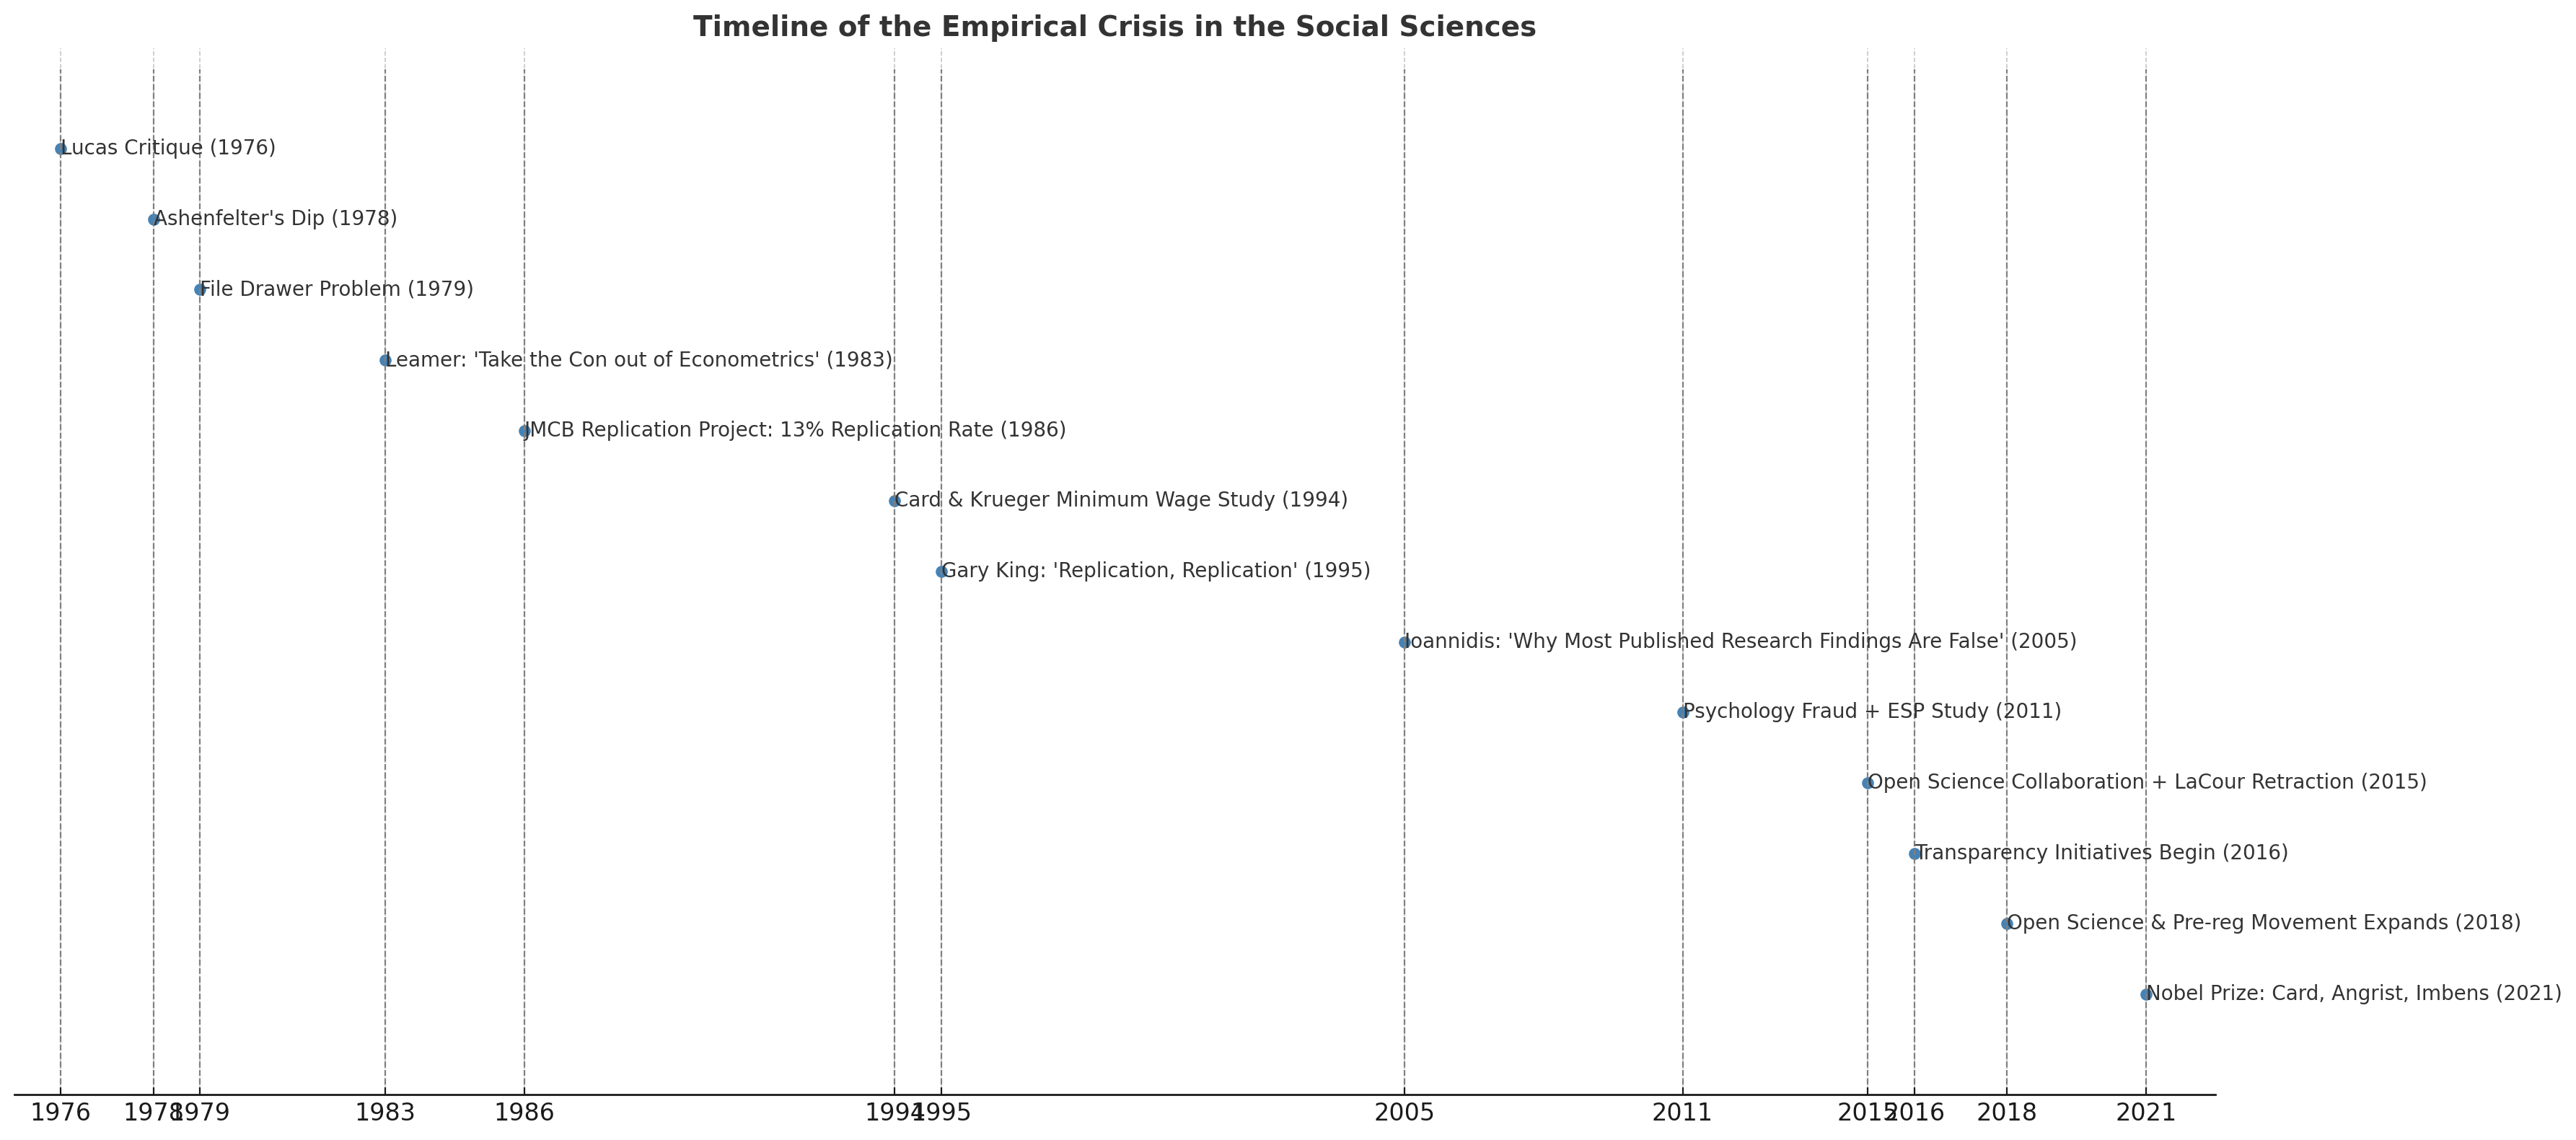
\includegraphics[height=0.5\textheight]{./lecture_includes/timeline}
\end{figure}

\end{frame}

\begin{frame}{Growing popularity in economics}

	\begin{figure}
	\caption{Currie, et al. (2020)}
	\includegraphics[scale=0.25]{./lecture_includes/currie_did.png}
	\end{figure}


\end{frame}















\begin{frame}{What is difference-in-differences (DiD)}

\begin{itemize}
\item DiD is when a group of units are assigned some treatment and then compared to a group of units that weren't before and after
\item One of the most widely used quasi-experimental methods in economics and increasingly in industry
\item Predates the randomized experiment by 80 years, but uses basic experimental ideas about treatment and control groups (just not randomized)
\item Uses panel or repeated cross section datasets, binary treatments usually, and often covariates
\end{itemize}
\end{frame}








\begin{frame}{Ignaz Semmelweis and washing hands}

\begin{itemize}
\item Early 1820s, Vienna passed legislation requiring that if a pregnant women giving birth went to a public hospital (free care), then depending on the day of week and time of day, she would be routed to either the midwife wing or the physician wing (most likely resulting in random assignment)
\item But by the 1840s, Ignaz Semmelweis noticed that pregnant women died after delivery in the (male) wing at a rate of 13-18\%, but only 3\% in the (female) midwife wing -- cause was puerperal or “childbed” fever
\item Somehow this was also we known -- women would give birth in the street rather than go to the physician if they were unlucky enough to have their water break on the wrong day and time
\end{itemize}

\end{frame}

\begin{frame}{Ignaz Semmelweis and washing hands}

\begin{itemize}
\item Ignaz Semmelweis conjectures after a lot of observation that the cause is the teaching faculty teaching anatomy using cadavers and then delivering babies \emph{without washing hands}
\item New training happens to one but not the other and Semmelweis thinks the mortality is caused by working with cadavers
\item Convinced the hospital to have physicians wash their hands in chlorine but not the midwives, creating a type of difference-in-differences design 
\end{itemize}

\end{frame}

\begin{frame}{Semmelweis diff-in-diff evidence}

	\begin{figure}
	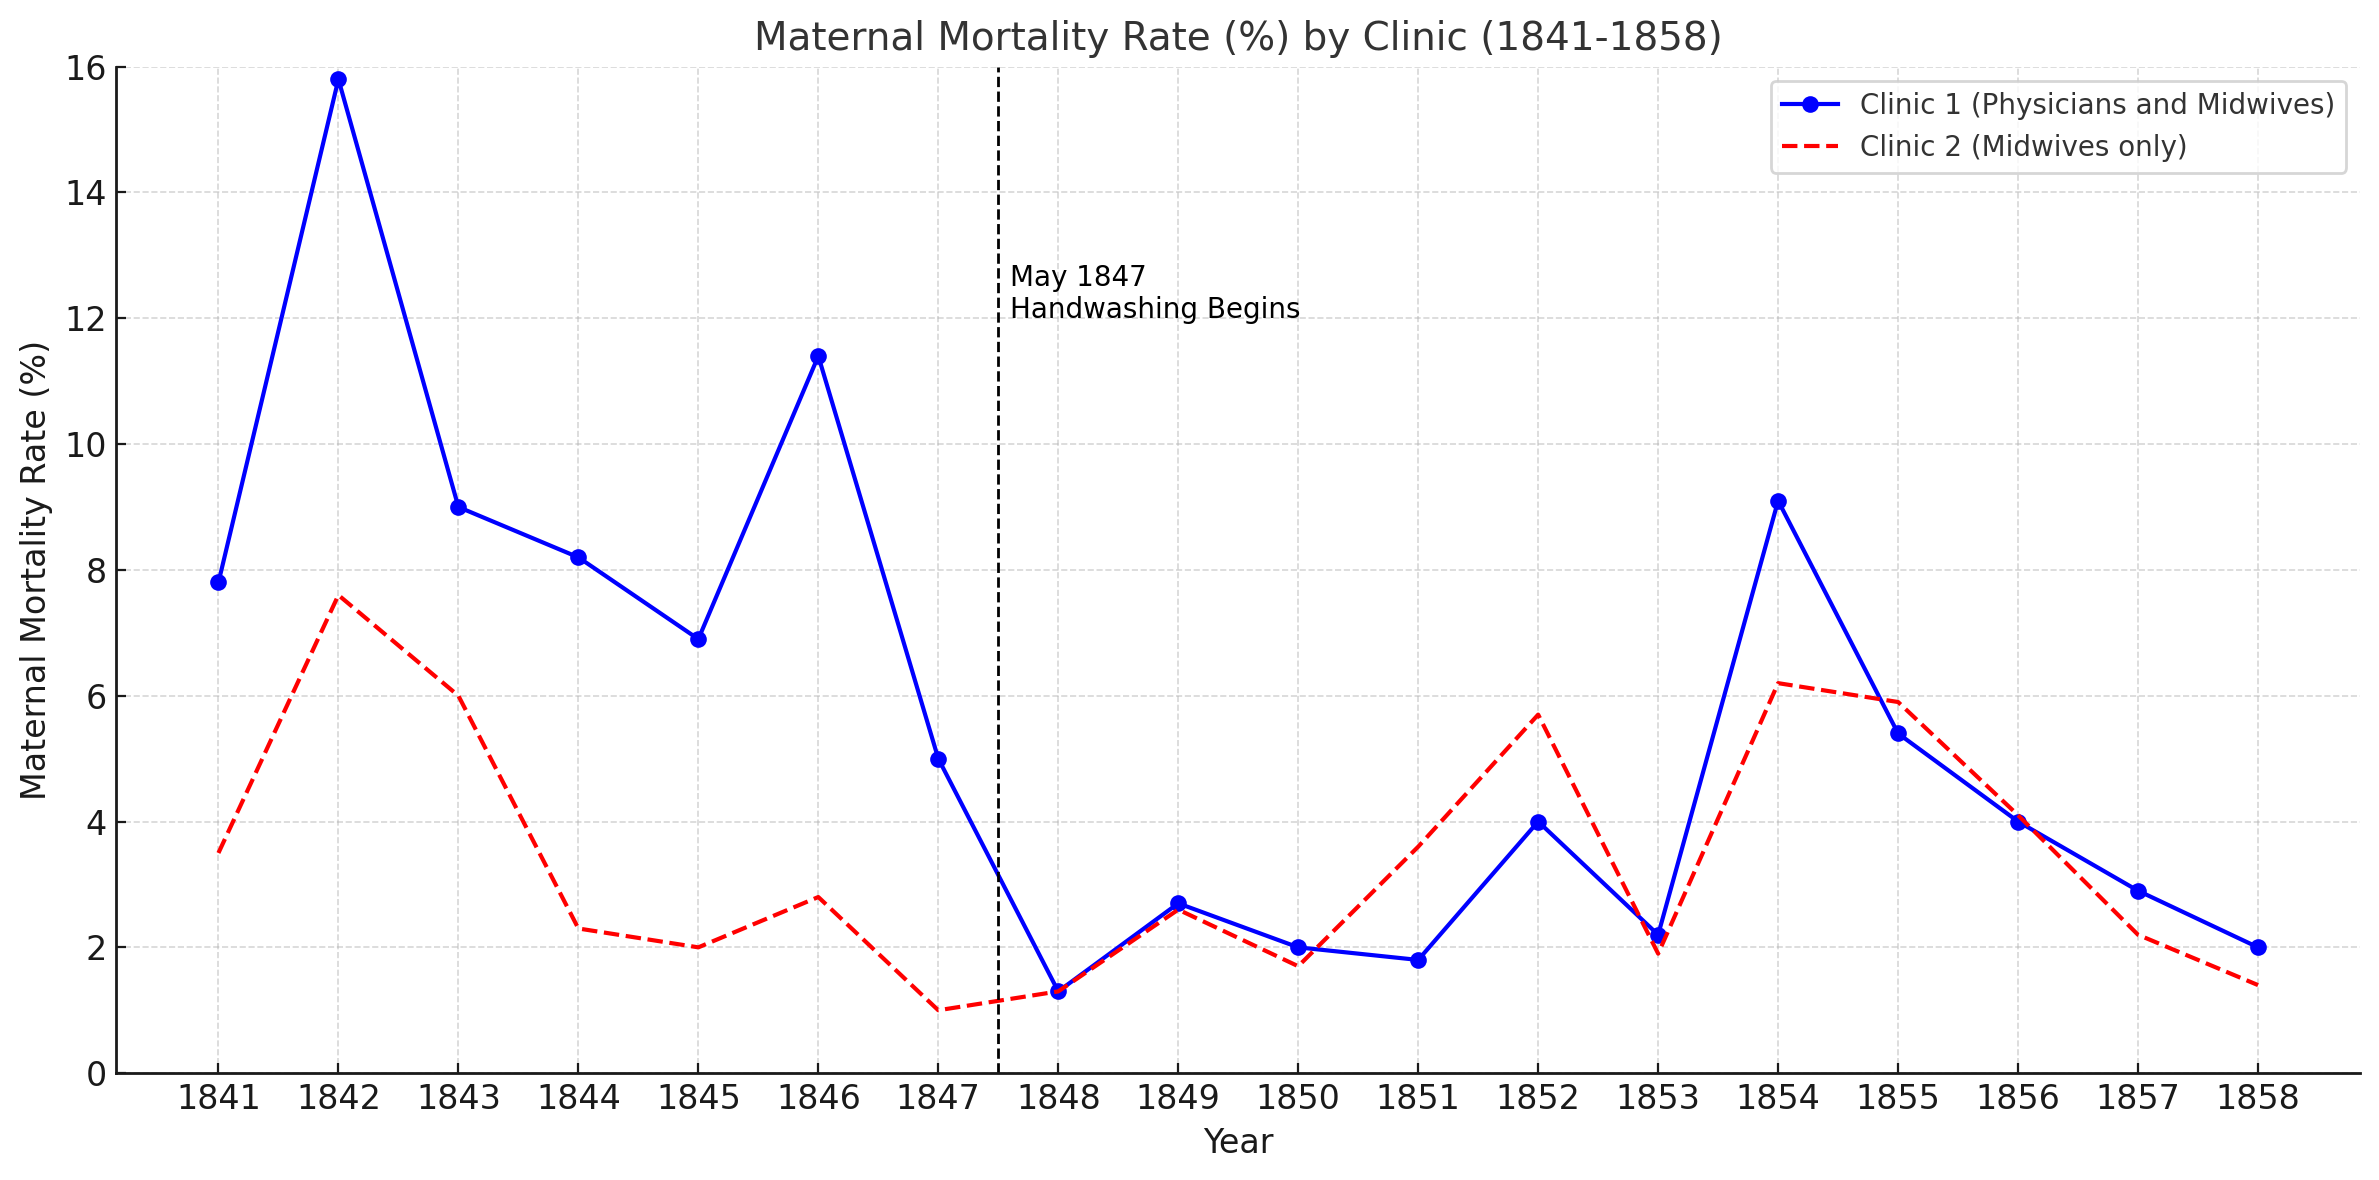
\includegraphics[scale=0.4]{./lecture_includes/semmelweis_graphic.png}
	\end{figure}


\end{frame}




\begin{frame}{John Snow and cholera}

\begin{itemize}
\item Three major waves of cholera in the early to mid 1800s in London, largely thought to be spread by miasma (``dirty air'')
\item John Snow believed cholera was spread through the Thames water supply through an invisible creature that entered the body through food and drink, caused the body to expel water, placing the creature back in the Thames and causing epidemic waves
\item London passes ordinance requiring water utility companies to move inlet pipe further up the Thames, above the city center, but not everyone complies
\item Natural experiment: Lambeth water company moves its pipe between 1849 and 1854; Southwark and Vauxhall water company delayed
\end{itemize}

\end{frame}


\begin{frame}

	\begin{figure}
	\caption{Two water utility companies in London 1854}
	\includegraphics[scale=0.225]{./lecture_includes/lambeth.png}
	\end{figure}


\end{frame}


\begin{frame}{Difference-in-differences}

\begin{table}\centering
\scriptsize
\caption{Lambeth and Southwark and Vauxhall, 1849 and 1854}
\begin{tabular}{lll|lc}
\toprule
\textbf{Companies} & \textbf{Time} & \textbf{Outcome} & $D_1$ & $D_2$ \\
\midrule
Lambeth & Before & $Y = L$ &  &  \\
        & After  & $Y = L + \textcolor{red}{L_t + D}$ & $\textcolor{red}{L_t + D}$ &  \\
\cmidrule{1-5}
Southwark and Vauxhall & Before & $Y = SV$ &  &  \\
                       & After  & $Y = SV + SV_t$ & $SV_t$ & $\textcolor{red}{(L_t + D - SV_t)}$ \\
\bottomrule
\end{tabular}
\end{table}

\begin{eqnarray*}
\widehat{\delta}_{did} = \textcolor{red}{D} + (\textcolor{red}{L_t} - SV_t)
\end{eqnarray*}

\end{frame}


\begin{frame}{Orley Ashenfelter}

\begin{itemize}

\item Orley Ashenfelter is a prominent labor economist at Princeton, was editor of the economics flagship journal \emph{American Economic Review}, and modern creator of diff-in-diff
\item Coins the phrase "difference-in-differences" so as to avoid having to explain regressions to bureaucrats (3:53)  \url{https://youtu.be/WnB3EJ8K7lg?si=uE4clqUIPzvbxm0r&t=2}
\item Advised several Nobel Laureates (Jim Heckman, David Card, Josh Angrist) and very influential through mentoring and leading the Princeton Industrial Relations Section in the 70s, 80s and 90s

\end{itemize}

\end{frame}



\subsection{Potential outcomes}




\begin{frame}{Four Averages and Three Subtractions}
$$Y_{ist} = \alpha_0 + \alpha_1 Treat_{is} + \alpha_2 Post_{t} + \textcolor{blue}{\delta} (Treat_{is} \times Post_t) + \varepsilon_{ist} $$

\bigskip

$$\widehat{\textcolor{blue}{\delta}} = \bigg ( \overline{y}_k^{post(k)} - \overline{y}_k^{pre(k)} \bigg ) - \bigg ( \overline{y}_U^{post(k)} - \overline{y}_U^{pre(k)} \bigg ) $$

\begin{itemize}
\item The OLS estimated coefficient, $\widehat{\delta}$, is numerically the same as "four averages and three subtractions"
\item Let's see that with a numerical example in \texttt{equivalence.do} and \texttt{equivalence.R}
\end{itemize}

\end{frame}

\begin{frame}{Introducing Potential Outcomes to DiD}

\begin{itemize}
\item Diff-in-diff is a simple calculation using data
\item But what is it estimating exactly?  To understand we need "causal language" and the most common these days is the potential outcomes model (Don Rubin)
\item I'll start with sentences then we will look at an exercise together
\end{itemize}

\end{frame}




\begin{frame}{Potential outcomes notation}
	
	\begin{itemize}
	\item Let the treatment be a binary variable: $$D_{i,t} =\begin{cases} 1 \text{ if in job training program $t$} \\ 0 \text{ if not in job training program at time $t$} \end{cases}$$where $i$ indexes an individual observation, such as a person

	\end{itemize}
\end{frame}

\begin{frame}{Potential outcomes notation}
	
	\begin{itemize}

	\item Potential outcomes: $$Y_{i,t}^j =\begin{cases} 1 \text{: wages at time $t$ if trained} \\ 0 \text{: wages at time $t$ if not trained} \end{cases}$$where $j$ indexes a state of the world where the treatment happened or did not happen

	\end{itemize}
\end{frame}



\begin{frame}{Treatment effect definitions}


	\begin{block}{Individual treatment effect}
	    The individual treatment effect,  $\delta_i$, equals $Y_i^1-Y_i^0$
	\end{block}

Missing data problem:  No data on the counterfactual 
	
\end{frame}




\begin{frame}{Average Treatment Effects for the Treated Subpopulation}	
	\begin{block}{Average Treatment Effect on the Treated (ATT)}
	The average treatment effect on the treatment group is equal to the average treatment effect conditional on being a treatment group member:
		\begin{eqnarray*}
		E[\delta|D=1]&=&E[Y^1-Y^0|D=1] \nonumber \\
		&=&E[Y^1|D=1]-\textcolor{red}{E[Y^0|D=1]}
		\end{eqnarray*}
	\end{block}
	
	\bigskip

It's the average causal effect but only for the people exposed to some intervention; notice we can't calculate it, also, because we are missing the red term

	
\end{frame}

\begin{frame}{Switching equation}

\begin{itemize}
\item Diff-in-diff is not estimated using potential outcomes, but rather "realized outcomes" (i.e., data)
\item Realized outcomes are the potential outcomes chosen by the treatment 

$$Y=D Y^1 + (1-D) Y^0$$

\item Moving between potential outcomes and realized outcomes is simply a matter of substitution 
\end{itemize}

\end{frame}


\begin{frame}{ATT vs ATE}

\begin{itemize}
\item Imagine there are 100 cities -- 25 of them raise the minimum wage, 75 do not
	\begin{itemize}
	\item ATE averages the treatment effects across all 100 cities (even though some don't)
	\item ATT averages the treatment effects for just the 25 cities that raised the minimum wage
	\end{itemize}
\item One of the first odd feelings you get with potential outcomes is the \emph{counterfactual} -- treatment effects are defined, based on events that don't happen, and yet we average them?
\item Can feel philosophical and even mysterious, and can often cause people to have to back up and start over
\item Let's review this with "Potential Outcomes" tab, \url{https://docs.google.com/spreadsheets/d/1hNxQX0qDNYYOfG-nGBvRuQJwUWDp-ayE7WK-cD7CgNA/edit?usp=sharing}
\end{itemize}

\end{frame}





\begin{frame}{DiD equation is the 2x2}

Orley's ``four averages and three subtractions'' uses two groups, two time periods, or 2x2

\begin{eqnarray*}
\widehat{\delta} = \bigg ( E[Y_k|Post] - E[Y_k|Pre] \bigg ) - \bigg ( E[Y_U | Post ] - E[ Y_U | Pre] \bigg) \\
\end{eqnarray*}$k$ are the people in the job training program, $U$ are the untreated people not in the program, $Post$ is after the trainees took the class, $Pre$ is the period just before they took the class, and $E[y]$ is mean earnings. 

\bigskip

When will $\widehat{\delta}$ equal the ATT?  When will it not?

\end{frame}



\begin{frame}{Replace with potential outcomes and add a zero}

\begin{eqnarray*}
\widehat{\delta} &=& \bigg ( \underbrace{E[Y^1_k|Post] - E[Y^0_k|Pre] \bigg ) - \bigg ( E[Y^0_U | Post ] - E[ Y^0_U | Pre]}_{\mathclap{\text{Switching equation}}} \bigg)  \\
&&+ \underbrace{\textcolor{red}{E[Y_k^0 |Post] - E[Y^0_k | Post]}}_{\mathclap{\text{Adding zero}}} 
\end{eqnarray*}

\end{frame}

\begin{frame}{Parallel trends bias}

\begin{eqnarray*}
\widehat{\delta} &=& \underbrace{E[Y^1_k | Post] - \textcolor{red}{E[Y^0_k | Post]}}_{\mathclap{\text{ATT}}} \\
&& + \bigg [  \underbrace{\textcolor{red}{E[Y^0_k | Post]} - E[Y^0_k | Pre] \bigg ] - \bigg [ E[Y^0_U | Post] - E[Y_U^0 | Pre] }_{\mathclap{\text{Non-parallel trends bias in 2x2 case}}} \bigg ]
\end{eqnarray*}


\end{frame}

\begin{frame}{Identification through parallel trends}
	

	\begin{block}{Parallel trends}
	Assume two groups, treated and comparison group, then we define parallel trends as:	 $$\textcolor{red}{E(}\textcolor{red}{\Delta Y^0_k)} = E(\Delta Y^0_U)$$
	\end{block}

\textbf{In words}: ``The \textcolor{red}{evolution of earnings for our trainees \emph{had they not trained}} is the same as the evolution of mean earnings for non-trainees''.  

\bigskip

It's in \textcolor{red}{red} because parallel trends is untestable and critically important to estimation of the ATT using any method, OLS or ``four averages and three subtractions''

\end{frame}

\begin{frame}{No Anticipation}

\begin{itemize}
\item ``No anticipation'' simply means that the unit is not treated in the "pre-period" of our diff-in-diff
	\begin{itemize}
	\item \textbf{Announced early}: If the law is announced before it is enacted, then you just need it to be that the treatment effect was zero in the pre-period
	\item \textbf{Announcement and Effective Dates the Same}: Makes pre-period untreated
	\end{itemize}
\item This is addressed in regressions by dropping the year that you want to be your baseline, and making sure that that year your treatment group was not yet treated
	
\end{itemize}

\end{frame}


\begin{frame}{No Anticipation Violation}


\begin{eqnarray*}
\widehat{\delta} &=& \bigg ( E[Y_k|Post] - E[Y_k|Pre] \bigg ) - \bigg ( E[Y_U | Post ] - E[ Y_U | Pre] \bigg) \\
\end{eqnarray*}

\bigskip

Add in \textbf{two zeroes} instead of one, substitute and rearrange.

\begin{eqnarray*}
&+& \textcolor{red}{E[Y^0_k|Post] - E[Y^0_k|Post]} \\
&+& \textcolor{blue}{E[Y^0_k|Pre] - E[Y^0_k|Pre]} 
\end{eqnarray*}

\end{frame}

\begin{frame}{No Anticipation Violation}

If the baseline period is treated, then the simple 2x2 identifies the following three terms:

\begin{eqnarray*}
\delta &=& ATT_k(Post) \\&&+ \text{Non PT bias} \\&&- \textcolor{blue}{ATT_k(Pre)}
\end{eqnarray*}

First row is the ATT in the post period; middle row is parallel trends; third row subtracts the baseline ATT from the calculation. If treatment effects are constant, then the DiD coefficient will be zero despite positive treatment effects.  Let's look in \texttt{na.do}.

\end{frame}

\begin{frame}{Do not use already treated controls}


\begin{eqnarray*}
\widehat{\delta} &=& \bigg ( E[Y_k|Post] - E[Y_k|Pre] \bigg ) - \bigg ( E[Y_U | Post ] - E[ Y_U | Pre] \bigg) \\
\end{eqnarray*}What if the $U$ group had always been treated in both periods? Is parallel trends enough to identify the ATT?

\bigskip

Add in \textbf{three zeroes} instead of one, substitute and rearrange.

\begin{eqnarray*}
&+& \textcolor{red}{E[Y^0_k|Post] - E[Y^0_k|Post]} \\
&+& \textcolor{blue}{E[Y^0_U|Post] - E[Y^0_U|Post]}  \\
&+& \textcolor{blue}{E[Y^0_U|Pre] - E[Y^0_U|Pre]} 
\end{eqnarray*}

\end{frame}

\begin{frame}{Already Treated Control Group}

If the baseline period is treated, then the simple 2x2 identifies the sum of the following three terms:

\begin{eqnarray*}
\delta &=& ATT_k(Post) \\&&+ \text{Non PT bias} \\&&- \textcolor{red}{\Delta ATT_U}
\end{eqnarray*}

Again, first row is the target parameter, plus parallel trends term, \textcolor{red}{minus} the changing ATT in our control group

\end{frame}



\subsection{Minimum wages}


\begin{frame}{Card and Krueger}

\begin{itemize}
\item Card and Krueger (1994) have a famous study estimating causal effect of minimum wages on employment
\item  New Jersey raises its minimum wage in April 1992 (between February and November) but neighboring Pennsylvania does not
\item Using DiD, they do not find a negative effect of the minimum wage on employment leading to complex reactions from economists
\item Orley's describes his understanding of people's reaction to the paper.  \\ \url{https://youtu.be/MOtbuRX4eyQ?t=1882}
\end{itemize}

\end{frame}

\begin{frame}
	\begin{figure}
	\includegraphics[scale=0.5]{./lecture_includes/minwage_whore}
	\end{figure}
\end{frame}


\begin{frame}{Reaction to the paper}


Lots of anecdotes in this interview with Card, but here are just two.  First, Card and Krueger received a lot of personal hostility from their peers (1:07 to 1:10)

\bigskip

\url{https://youtu.be/1soLdywFb_Q?si=laAVYf_E2KBZKywG&t=4020}

\bigskip

Later Card says Sherwin Rosen accused them of having an agenda.  But the worst is what happens to Alan Krueger maybe (1:16 to 1:17)

\bigskip

\url{https://youtu.be/1soLdywFb_Q?si=jsb8h50ZosGDnKrv&t=4556}




\end{frame}

\begin{frame}{Card on that study}

\begin{quote}
``I’ve subsequently stayed away from the minimum wage literature for a number of reasons. First, it cost me a lot of friends. People that I had known for many years, for instance, some of the ones I met at my first job at the University of Chicago, became very angry or disappointed. They thought that in publishing our work we were being traitors to the cause of economics as a whole.''
\end{quote}


\end{frame}



\begin{frame}{OLS specification of the DiD equation}
	
	\begin{itemize}
	\item The correctly specified OLS regression is an interaction with time and group fixed effects:$$Y_{its} = \alpha + \gamma NJ_s + \lambda d_t + \delta (NJ \times d)_{st} + \varepsilon_{its}$$
		\begin{itemize}
		\item NJ is a dummy equal to 1 if the observation is from NJ
		\item d is a dummy equal to 1 if the observation is from November (the post period)
		\end{itemize}
	\item This equation takes the following values
		\begin{itemize}
		\item PA Pre: $\alpha$
		\item PA Post: $\alpha + \lambda$
		\item NJ Pre: $\alpha + \gamma$
		\item NJ Post: $\alpha + \gamma + \lambda + \delta$
		\end{itemize}
	\item DiD equation: (NJ Post - NJ Pre) - (PA Post - PA Pre) $= \delta$
	\end{itemize}
\end{frame}




\begin{frame}[plain]
	$$Y_{ist} = \alpha + \gamma NJ_s + \lambda d_t + \delta(NJ\times d)_{st} + \varepsilon_{ist}$$
	\begin{figure}
	\includegraphics[scale=0.90]{./lecture_includes/waldinger_dd_5.pdf}
	\end{figure}
\end{frame}


\begin{frame}[plain]
	$$Y_{ist} = \alpha + \gamma NJ_s + \lambda d_t + \delta(NJ\times d)_{st} + \varepsilon_{ist}$$
	\begin{figure}
	\includegraphics[scale=0.90]{./lecture_includes/waldinger_dd_5.pdf}
	\end{figure}

Notice how OLS is ``imputing'' $E[Y^0|D=1,Post]$ for the treatment group in the post period? It is only ``correct'', though, if parallel trends is a good approximation

\end{frame}






\begin{frame}{Conservative inference in DiD}
  \begin{itemize}
	\item  Bertrand, Duflo and Mullainathan (2004) show that conventional standard errors will often severely understate the standard deviation of the estimators
	\item They proposed three solutions, but most only use one of them (clustering)
	    \item Clustering standard errors accounts for this within-cluster correlation and is a more conservative approach 
	    \item Clustering is typically recommended at the aggregate unit where the entire treatment occurred

  \end{itemize}
\end{frame}




\subsection{Event studies}

\begin{frame}{Parallel Trends is not Verifiable}

\begin{itemize}
\item If "unconditional parallel trends" (meaning no covariates included in your model) holds, then four averages and three subtractions is causal
\item But parallel trends is not observed -- let's go over an example together so that we can understand this better
\item \url{https://docs.google.com/spreadsheets/d/1hNxQX0qDNYYOfG-nGBvRuQJwUWDp-ayE7WK-cD7CgNA/edit?usp=sharing}
\end{itemize}

\end{frame}


\begin{frame}{Evidence, not proof}

\begin{itemize}
\item Think of event studies as \emph{evidence}, not \emph{proof}
	\begin{itemize}
	\item Prosecutor claims the defendant is guilty
	\item But the evidence is not the claim -- claim must be supported with evidence
	\item Evidence is witnesses, fingerprints, DNA, muddy boot prints
	\end{itemize}
\item Event studies are evidence of pre-trends only, and they are used both as a falsification and make clear that you are taking a stand on who the control group is and why
\end{itemize}
\end{frame}





\begin{frame}{Creating event studies}

\begin{itemize}

\item You want to visualize a particularly set of regression coefficients which we will show
\item But if you can show the raw data, do that too as that will show difference in levels as well which will matter for the next section on covariates

\end{itemize}

\end{frame}



\begin{frame}

	\begin{figure}
	\includegraphics[scale=2.5]{./lecture_includes/waldinger_dd_6.pdf}
	\end{figure}

\end{frame}


\begin{frame}{Event study regression}
	
	\begin{itemize}
	\item Alternatively, present estimated coefficients from a dynamic regression specification:
 $$Y_{its} = \alpha + \sum_{\tau=-2}^{-q}\mu_{\tau} (D_s \times \tau_t) + \sum_{\tau=0}^m\delta_{\tau} (D_s \times \tau_t) + \tau_t + D_s + \varepsilon_{ist}$$
		\begin{itemize}
		\item With a simple 2x2, you are interacting treatment indicator with calendar year dummies
		\item Includes $q$ leads (dropping the $t-1$ as baseline) and $m$ lags 
		\item Since treatment did not happen until $\tau=0$, then pre-treatment coefficients only capture differential trends
		\end{itemize}
	\item Estimated $\widehat{\delta}_\tau$ coefficients are estimated ATT for each year under parallel trends but $\widehat{\mu}_\tau$ is your smoking gun evidence 
	\item Just remember that $\mu=0$ is not the same as parallel trends as parallel trends is \textcolor{red}{untestable}.
	\end{itemize}
\end{frame}

\begin{frame}{Reviewing previous slide for emphasis}


\begin{itemize}
\item Under NA, SUTVA and parallel pre-trends, then mechanically $\widehat{\mu_{\tau}}$ will be zero as everything cancels out
	\begin{itemize}
\item There are still specification and power issues that Jon Roth has written about, but I will skip that
	\end{itemize}
\item But also under NA, SUTVA and parallel trends (post trends), then $\widehat{\delta}$ are estimates of the ATT at points in time
\item  Typically you'll plot the coefficients and 95\% CI on all leads and lags
\end{itemize}

\end{frame}

\begin{frame}{Normal DiD coefficient}

\begin{eqnarray*}
\widehat{\delta} &=& \underbrace{E[Y^1_k | Post] - \textcolor{red}{E[Y^0_k | Post]}}_{\mathclap{\text{ATT}}} \\
&& + \bigg [  \underbrace{\textcolor{red}{E[Y^0_k | Post]} - E[Y^0_k | Pre] \bigg ] - \bigg [ E[Y^0_U | Post] - E[Y_U^0 | Pre] }_{\mathclap{\text{Non-parallel trends bias in 2x2 case}}} \bigg ]
\end{eqnarray*}

\bigskip

But this was \emph{post}-treatment.  Still, put that aside -- diff-in-diff equations \emph{always} identify the sum of those terms, even in the pre-period


\end{frame}

\begin{frame}{Pre-treatment DiD coefficient}

\begin{eqnarray*}
\widehat{\delta}_{t-2} &=& \bigg [  \underbrace{\textcolor{black}{E[Y^0_k | t-2]} - E[Y^0_k | t-1] \bigg ] - \bigg [ E[Y^0_U | t-2] - E[Y_U^0 | t-1] }_{\mathclap{\text{Non-parallel trends bias in 2x2 case}}} \bigg ]
\end{eqnarray*}

\bigskip

Under NA, then the $t-1$ period is untreated.  But then so are the other pre-periods so the ATT is implicitly zero and the \emph{only} thing that you can be measuring with pre-trend DiD coefficients is differential trends.  


\end{frame}




\begin{frame}{Event study example}

\begin{itemize}
\item The notion is really simple: if PT held then, you'll argue that it's reasonable it would've still held
\item But this is an assertion, and you need to build the case as we said
\item At this point, it's a lot easier to show you what I'm talking about -- where the art and the science meet -- with a great paper
\end{itemize}

\end{frame}




\begin{frame}{Medicaid and Affordable Care Act example}

\begin{figure}
\includegraphics[scale=0.25]{./lecture_includes/medicaid_qje}
\end{figure}

\end{frame}
\begin{frame}{Their Evidence versus Their Result}

\begin{itemize}
\item \textbf{Bite} -- they will show that the expansion shifted people into Medicaid and out of uninsured status
\item \textcolor{black}{\textbf{Falsifications}} -- they show that there's no effect of Medicaid on a similar group that didn't enroll
\item \textbf{Event study} -- they will lean hard on those dynamic plots
\item \textcolor{red}{\textbf{Main results}} -- with all of this, they will show Medicaid expansion caused near elderly mortality to fall
\item \textcolor{black}{\textbf{Mechanisms}} -- they think they can show it's coming from people treating diseases causing mortality declines to compound over time
\end{itemize}

\end{frame}

\begin{frame}{Bite}

\begin{itemize}
\item Bite is a labor economist's phrase, often used with the minimum wage, to say that the minimum wage actually was binding in the first place
\item Here it means when US states made Medicaid more generous, people got on Medicaid who would not have been on it otherwise
\item And as a bonus, would not have been insured at all without it
\item Not the most exciting result, but imagine if the main results on mortality were shown but there was no evidence for bite -- is it believable?
\end{itemize}

\end{frame}


\imageframe{./lecture_includes/Miller_Medicaid1.png}

\imageframe{./lecture_includes/Miller_Medicaid2.png}

\imageframe{./lecture_includes/Miller_Medicaid3.png}


\begin{frame}{Falsification}

\begin{itemize}

\item Their study focuses on ``near elderly'', which means just under 65
\item They choose just under 65 because in the US, 65 and older are eligible for Medicare so more generous Medicaid is irrelevant
\item \emph{But} probably the near elderly and the elderly are equally susceptible to unobserved factors correlated with the treatment
\item So they painstakingly examine the effects on elderly as a falsification as this will strengthen the parallel trends assumption on the near elderly
\end{itemize}

\end{frame}

\begin{frame}{Falsifications on elderly}

	\begin{figure}
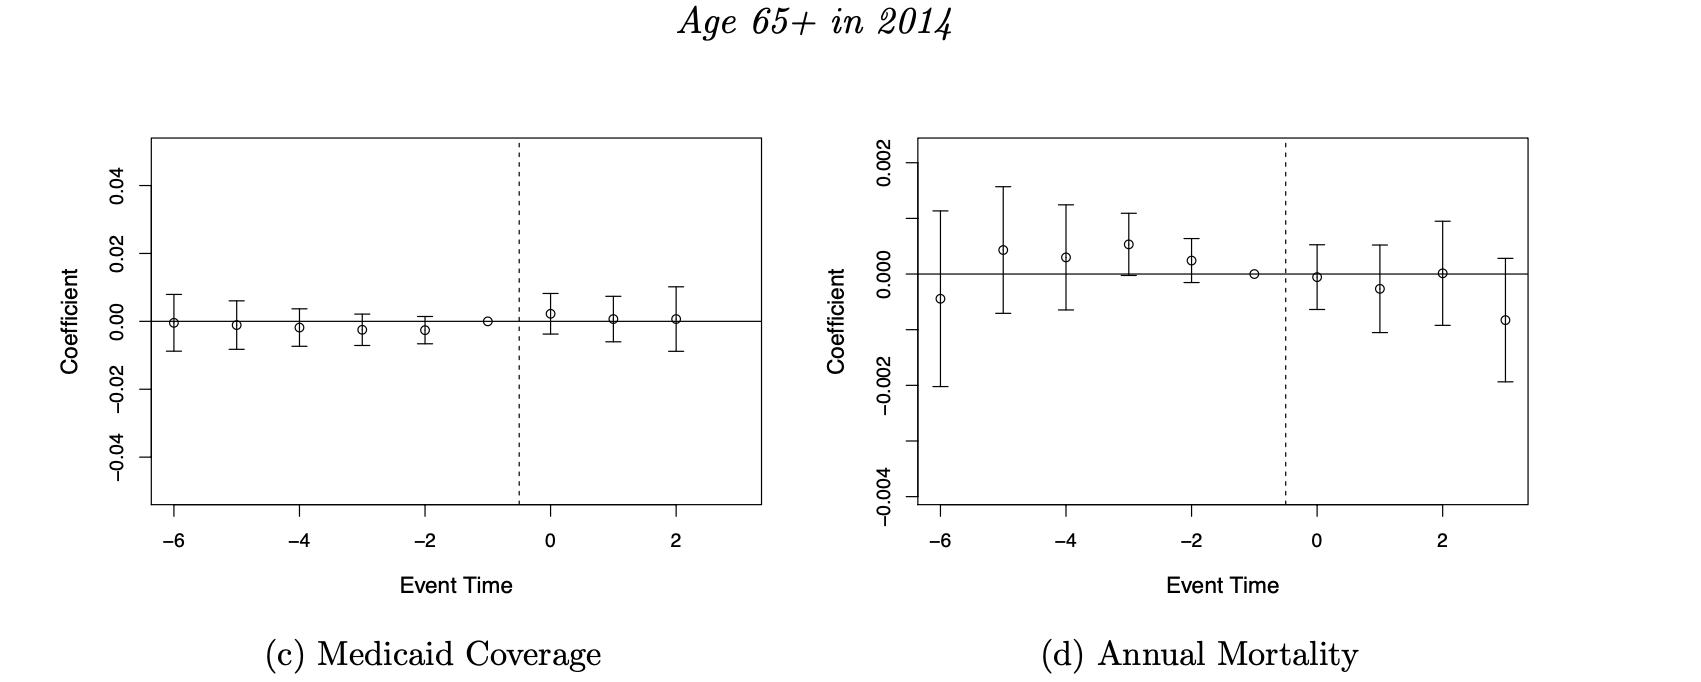
\includegraphics[scale=0.425]{./lecture_includes/placebo_medicaid}
	\end{figure}

\end{frame}

\begin{frame}{Main result}

\begin{itemize}

\item Finally they focus on the main result -- and there's more in the paper than I'm showing
\item Event study plots with same specification as the rest allowing us to look at the pre-trends and the post-treatment coefficients
\item If parallel trends holds, then the post-treatment coefficients are interpreted as ATT parameter estimates for each time period
\item The result alone isn't nearly as strong the result in combination with the rest, but it could still be wrong as parallel trends is ultimately not verfiable
\end{itemize}

\end{frame}



\begin{frame}{Near elderly mortality and Medicaid expansion}

	\begin{figure}
	\includegraphics[scale=0.3]{./lecture_includes/Miller_Medicaid4.png}
	\end{figure}

\end{frame}

\begin{frame}{Summarizing evidence and results}

\begin{itemize}
\item \textbf{Bite}: Increases in enrollment and reductions in uninsured support that there is adoption of the treatment
\item \textbf{Event studies}: Compelling graphics showing similarities between treatment and control
\item \textbf{Falsifications}: no effect on a similar group who isn't eligible
\item \textcolor{red}{Main results}: 9.2\% reduction in mortality among the near-elderly
\item \textcolor{red}{Mechanism}: ``The effect is driven by a reduction in disease-related deaths and grows over time.''
\end{itemize}

\end{frame}

\begin{frame}{Making event study}

\begin{itemize}
\item When there is only one treatment group and one comparison group, then you run a regression with an interaction of the treatment group dummy and the calendar year dummies (plus both separately)
\item You must drop $t-\tau$ as the baseline (e.g., $t-1$) and it must be $Y^0$ untreated comparisons (No Anticipation)
\item I have included in a do file that will do it for you either manually or using coefplot in \texttt{simple\_eventstudy.do} and .R at the shared github labs directory
\end{itemize}

\end{frame}


\begin{frame}{Manually creating the event study}

	\begin{figure}
	\includegraphics[scale=0.20]{./lecture_includes/simple_eventstudy_manual}
	\end{figure}

\end{frame}



\section{Covariates}

\subsection{Conditional parallel trends}

\begin{frame}{Unconditional vs conditional parallel trends}

\begin{itemize}
\item Assume male earnings grow at $+2$ per year and female earnings grow at $+1$ a year
\item Assume your treatment group is 75\% male but your control group is 25\% male
\begin{enumerate}
\item \textbf{Treatment group trend}: $\Delta E[Y^0|D=1] = 1.75$
\item \textbf{Control group trend}:  $\Delta E[Y^0|D=0] = 1.25$
\end{enumerate}
\item Simply the fact that the two groups have different trends \emph{and} the composition of the two groups being difference \textcolor{red}{breaks parallel trends}
\end{itemize}

\end{frame}



\begin{frame}{Why include controls?}

\begin{itemize}
\item Two reasons to include controls
	\begin{enumerate}
	\item \textbf{Conditional parallel trends}: Parallel trends only holds for the sub-populations (i.e., males) and the groups are imbalanced (i.e., 75\% vs 25\% males)
	\item \textbf{Precision}: Covariates are highly predictive of your outcome can shrink confidence intervals and standard errors
	\end{enumerate}
\item But how do we incorporate the covariates into the model? 
\end{itemize}

\end{frame}



\begin{frame}{Conditional parallel trends}
Conditional parallel trends (CPT) is a weakened version of the parallel trends assumption requiring that it holds \emph{within} the dimensions of the selected covariates:
\begin{align*}
CPT: \textcolor{red}{E[Y^0_k|Post, X]} - E[Y^0_k|Pre, X] = E[Y^0_U|Post, X] - E[Y^0_U|Pre, X]
\end{align*}
\end{frame}




\begin{frame}{Which covariates do you need?}

\begin{itemize}
\item Conditional parallel trends is tricky because it first assumes you know the covariates you need to satisfy it
\item But how do we decide which variables do this and which ones don't?
\item Econometrics is no help here -- you need common sense, theory, logic, and expertise
\item When selecting covariates, use "confounders" logic and perhaps a graph
\end{itemize}

\end{frame}
	



\begin{frame}{Graphs Can Help Pick Covariates}

\begin{figure}[h!]
    \centering
    \begin{tikzpicture}[
        node distance=2.5cm,
        every node/.style={align=center},
        line/.style={->, thick},
    ]
    % Nodes
    \node (X) {Covariates \\ \( X \)};
    \node (D) [below left of=X, xshift=-1cm, yshift=-1cm] {\( D \)};
    \node (DeltaY0) [below right of=X, xshift=1cm, yshift=-1cm] {\( \Delta E\left[Y^0\right] \)};
    % Arrows
    \draw[line] (X) -- (DeltaY0);
    \draw[line] (X) -- (D);
    \end{tikzpicture}
\caption{DAG representing differences in county-level covariate composition (\(X\)) across treatment and control groups (\(D\)) and their determination of the untreated potential outcome trends (\(\Delta E\left[Y^0\right]\)).}
\end{figure}

\end{frame}



\begin{frame}{Covariate Imbalance}
    \begin{itemize}
    \item DAG $X \rightarrow Y^0$ was about picking covariates that ordinarily cause different trends in the untreated potential outcome
    \item But next we have to figure out whether the covariates are imbalanced
\item For that, we focus on $X \rightarrow D$, which is to say, check the imbalance in covariates you need for conditional parallel trends
\end{itemize}
\end{frame}



\begin{frame}{Create a balance table}

\begin{figure}
    \centering
    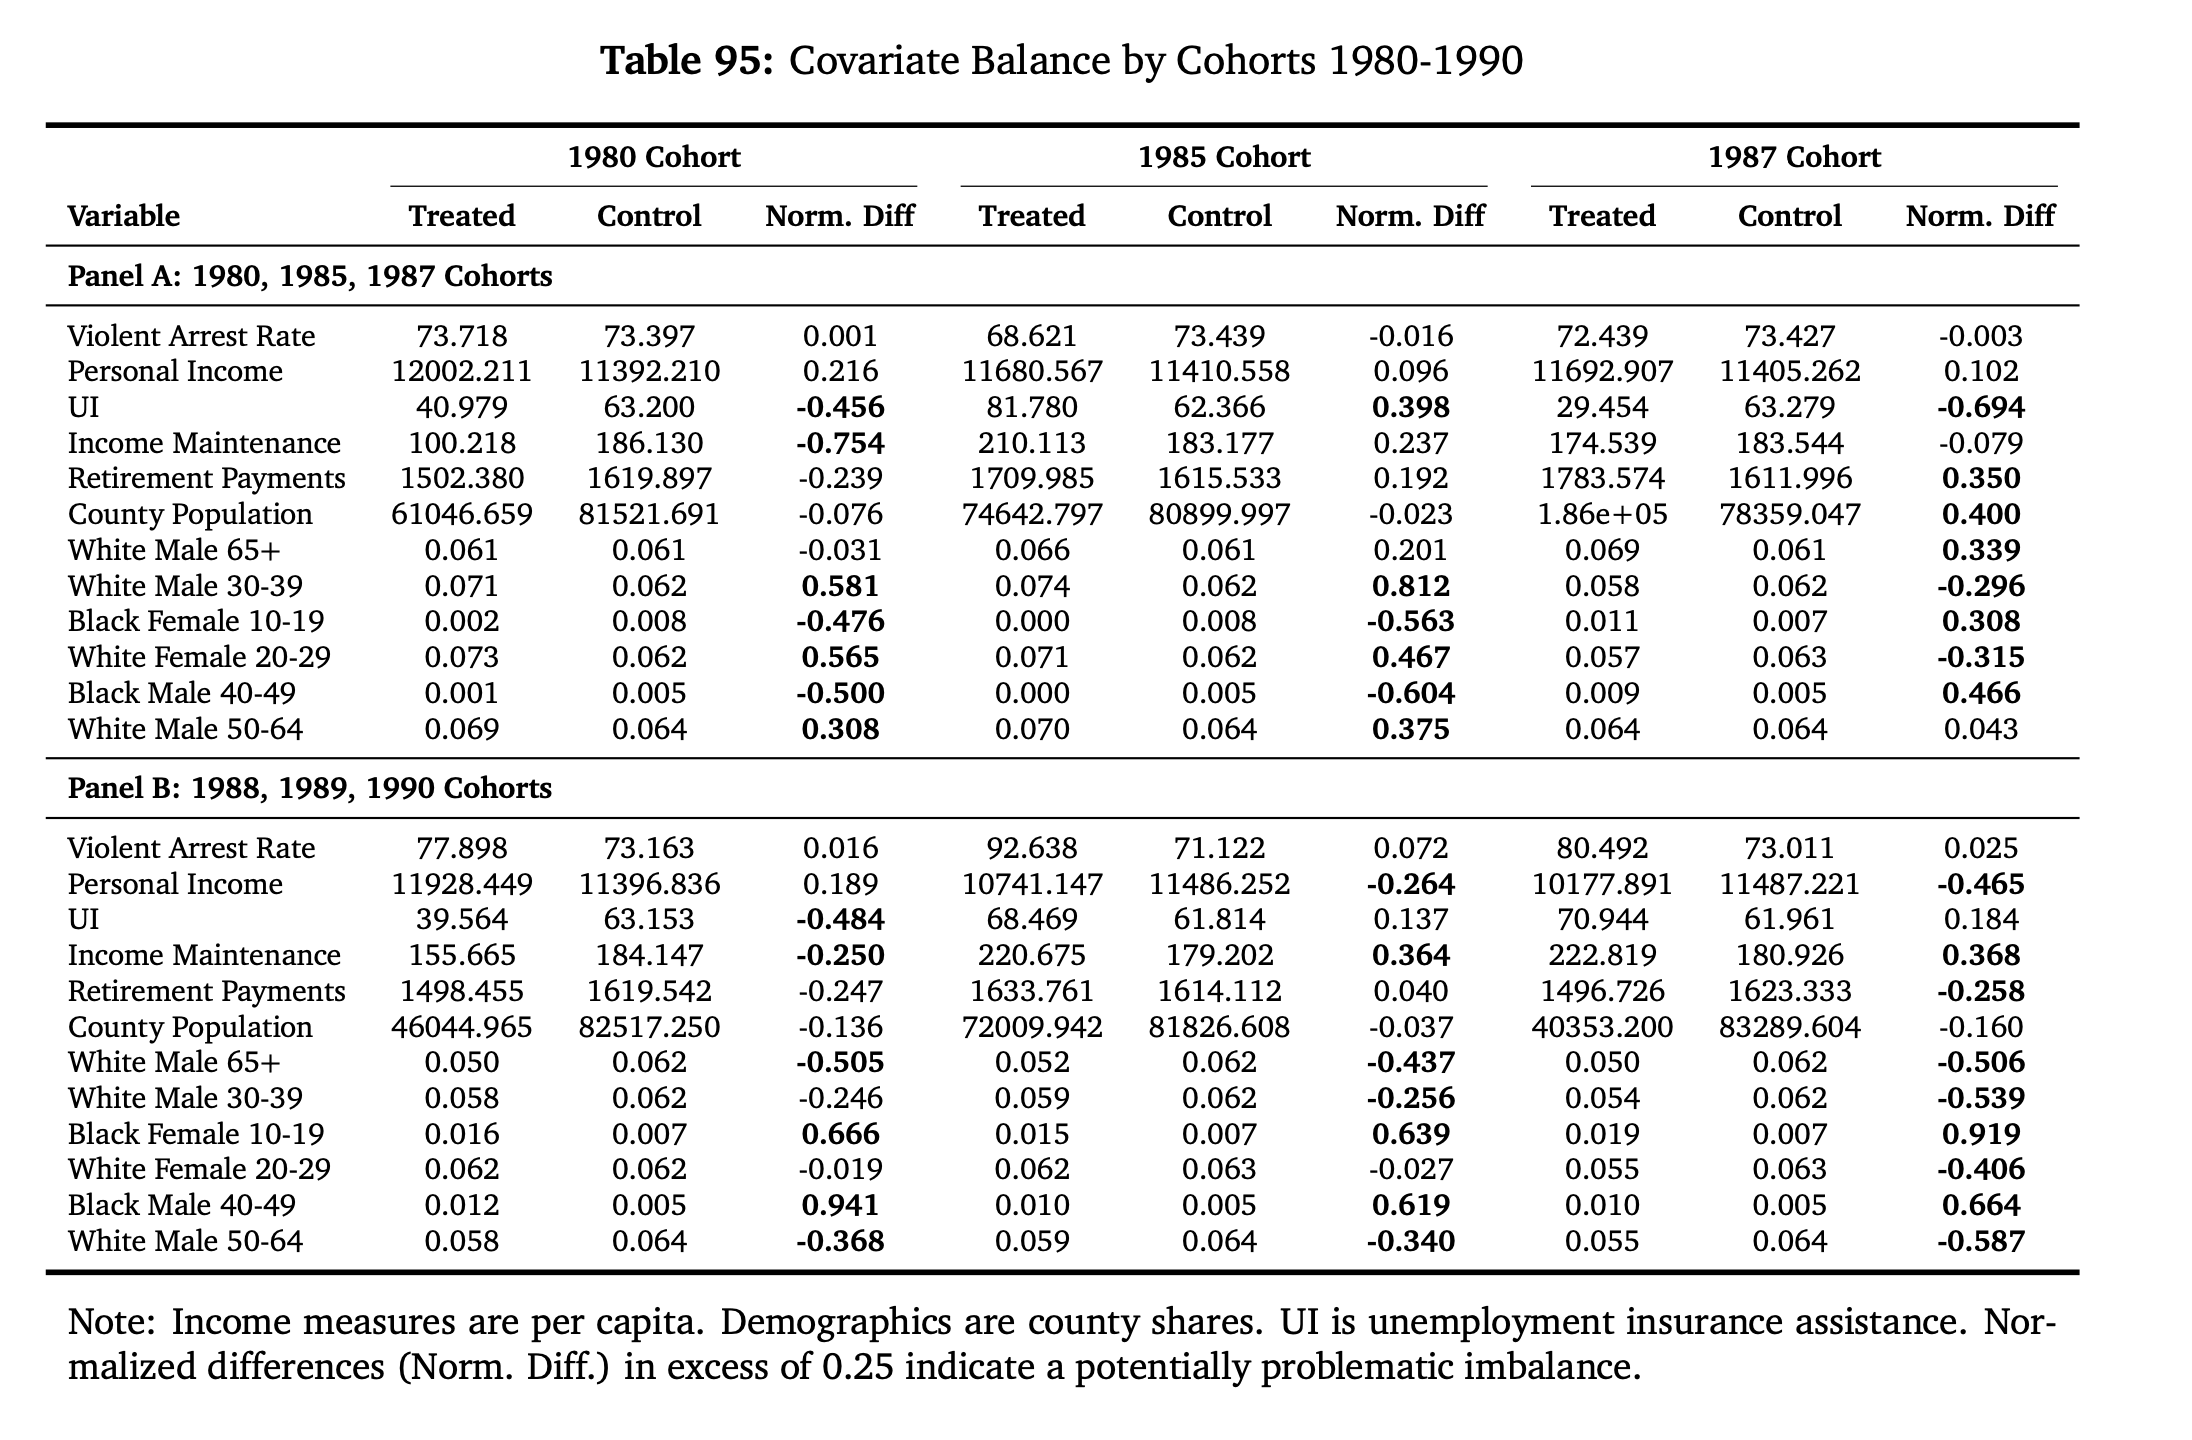
\includegraphics[height=0.80\textheight]{./lecture_includes/step6_imbalance}
\end{figure}

\end{frame}


\begin{frame}
    \frametitle{Baseline Covariates and Normalized Difference}
    \begin{itemize}
        \item Baseline covariates are measured before treatment ($t-1$). 
        \item Report the averages of covariates for both groups in a table and the "normalized difference in means" calculated as:
        $$ \text{Norm. Diff}_\omega = \frac{\overline{X}_{\omega,T} - \overline{X}_{\omega,C}}{\sqrt{(S_{\omega,T}^2 + S_{\omega,C}^2)/2}} $$
        \item The normalized difference measures imbalance; it should be less than 0.25 in absolute value to avoid problematic imbalance (Imbens and Rubin 2015).
    \end{itemize}
\end{frame}


\begin{frame}{Summarizing}
    \begin{itemize}
    \item So, when choosing covariates, remember that there are two steps involved
    	\begin{enumerate}
	\item $X \rightarrow \Delta E[Y^0]$. Pick covariates that are needed to satisfying conditional parallel trends 
	\item $X \rightarrow D$. Check for imbalance using the normalized difference in means equation to determine if you have "problematic imbalance"
	\end{enumerate}
\item And the heuristic I am suggesting is to select covariates that are the "ordinary determinants of $Y^0$" (i.e., become an expert on your left-hand-side variable)
    \end{itemize}
\end{frame}

 






\subsection{Four Estimators for Covariates}



\begin{frame}{Estimators for Covariates}

\begin{itemize}

\item What estimators can accommodate that assumption with the least amount of assumptions?
	\begin{enumerate}
	\item Inverse probability weighting
	\item Outcome regression
	\item Double robust
	\item Regressions
	\end{enumerate}
\item We will have code and calculations
\end{itemize}

\end{frame}







\begin{frame}{Inverse probability weighting}


 Abadie (2005) proposed a model that simply reweights the control group in the DiD equation using a particular specification (``semiparametric'') of the propensity score on pretreatment covariates
 
	\begin{enumerate}
	\item Calculate each unit's ``after minus before'' (DiD equation)
	\item Estimate the conditional probability of treatment based on baseline covariates (propensity score estimation)
	\item Weight the comparison group's DiD equation with the propensity score 
	\end{enumerate}

Remember -- ATT is only missing $Y^0$ for treatment, so we only have to apply weights to the comparison group units

\end{frame}

\begin{frame}{Novel elements of time in Abadie's model}

\begin{itemize}
\item There is only one treatment group so therefore there is only one relevant treatment date, $t$
\item The period prior to treatment is called the baseline, or $b$, period and it is when treated units were not treated 
\item $X_b$ are ``baseline'' covariates meaning the value of $X$ in the pre-treatment period for either the treated or comparison group units
\item Propensity scores are estimated off the $b$ period \emph{only} 
\item Abadie ``throws away'' covariates after treatment because this is all about re-establishing parallel trends which is a \emph{baseline} concept recall
\end{itemize}

\end{frame}

\begin{frame}{Assumptions}

Five main assumptions

\begin{enumerate}
\item No anticipation 
\item Untreated control group
\item Conditional parallel trends $$E[Y^0_t - Y^0_b|D=1,X_b] = E[Y^0_t - Y^0_b | D=0, X_b]$$ 
\item Common support $$Pr(D=1)>0; Pr(D=1|X)<1$$ 
\item Propensity score model is properly specified 
\end{enumerate}

\end{frame}

\begin{frame}{Propensity scores as dimension reduction}

\begin{itemize}

\item Propensity scores are ways of dealing with a conditioning set $X$ that has large dimensions
\item Dimensions are not the same as covariates -- if you have continuous $X$, then it has infinite dimensions
\item Common support means that \emph{within} all combinations of the covariates (e.g., white male 47yo versus whites, males, age) there are units in treatment and control

\end{itemize}

\end{frame}

\begin{frame}{Common support example}

Think of common support like ``exact matches'' but on the propensity score

\bigskip

I'm a white male 47 years old with a PhD; can I find a white male 47 years old without a PhD

\bigskip

If I can, that's common support; if I cannot that's off support

\end{frame}




\begin{frame}{How do these work together?}

Since we are identifying the ATT, and the ATT is missing $Y^0$ for the treated group, we are using the control group $Y^0$ in its place 

\bigskip

Under conditional parallel trends and common support, some of the comparison group units are recovering the parallel trends because of their $X$ values creating projections that in their differences perfectly aligned in expectation with the missing $\Delta E[Y^0|D=1]$

\bigskip

But we have to have all three for it to work

\end{frame}

\begin{frame}{Visualizing propensity score to get common support}

	\begin{figure}
	\includegraphics[scale=0.05]{./lecture_includes/common_support_abadie.png}
	\end{figure}

\end{frame}

\begin{frame}{Definition and estimation}

Defining the ATT parameter of interest
\begin{eqnarray*}
ATT &=& E[Y^1_t - \textcolor{red}{Y^0_t} |D=1] \\
&=&E[Y^1_t  | D = 1 ] - \textcolor{red}{E[Y^0_t | D=1]}
\end{eqnarray*}

\bigskip
Abadie's inverse probability weighting (IPW) estimator
\begin{eqnarray*}
E\bigg [ \frac{Y_t - Y_b}{Pr(D=1)} \times \frac{D - Pr(D=1|X_b)}{1-Pr(D=1|X_b)} \bigg ]
\end{eqnarray*}

\bigskip

The first is our causal parameter; the second is our reweighted DiD equation that \emph{estimates} our causal parameter, but we need to estimate that propensity score


\end{frame}

\begin{frame}{Abadie's IPW estimator}

Look closely; what happens mathematically when you substitute $D=1$ vs $D=0$?

\begin{eqnarray*}
E\bigg [ \frac{Y_t - Y_b}{Pr(D_t=1)} \times \frac{D_t - Pr(D=1|X_b)}{1-Pr(D=1|X_b)} \bigg ]
\end{eqnarray*}

\bigskip

The reweighting with the propensity only happens to the comparison group's first differences -- not the treatment groups!  Why?  Because it's the $Y^0$ that is missing, not the $Y^1$

\end{frame}









\begin{frame}{Outcome Regression and Double Robust}

\begin{itemize}
\item Another method developed by Heckman, Ichimura and Todd (1997) imputes the missing counterfactual using covariate relationships with the outcome in the control group
\item I will discuss this in the context of a method that will do both the regression imputation method off covariates and the the IPW method at the same time
\item I'll then compare all three with vanilla OLS specifications and include a simulation and example code

\end{itemize}
\end{frame}

\begin{frame}{Outcome Regression and Double Robust}

\begin{itemize}
\item DR models control for covariates twice -- once using the propensity score, once using outcomes adjusted by regression -- and are unbiased so long as:
	\begin{itemize}
	\item The regression specification for the outcome is correctly specified
	\item The propensity score specification is correctly specified
	\end{itemize}
\item Sant'Anna and Zhao (2020) incorporated DR into DiD by combining inverse probability weighting and outcome regression into a single DiD model
\item It's in the engine of Callaway and Sant'Anna (2020) that we discuss later so it merits close study
\end{itemize}

\end{frame}




\begin{frame}{Identification assumptions I: Data}

Assumption 1: Assume panel data or repeated cross-sectional data

\bigskip

Handling repeated cross-sectional data is possible but assumes stationarity which is a kind of stability assumption, but I'll use panel representation. 

\bigskip

Cross-sections will be potentially violated with changing sample compositions (e.g., the Napster example). 

\end{frame}

\begin{frame}{Identification assumptions II: Modification to parallel trends}

Assumption 2: Conditional parallel trends

\bigskip

Counterfactual trends for the treatment group are the same as the control group for all values of $X$

\begin{eqnarray*}
E[Y_1^0 - Y_0^0 | X, D=1] = E[Y^0_1 - Y^0_0 | X, D=0]
\end{eqnarray*}

\end{frame}

\begin{frame}{Identification assumptions III: Common support}

Assumption 3: Common support

\bigskip

For some $e>0$, the probability of being in the treatment group is greater than $e$ and the probability of being in the treatment group conditional on $X$ is $\leq1-e$. 

\bigskip

Heckman, et al doesn't use the propensity score so we need a more general expression of support

\end{frame}

\begin{frame}{Estimating DD with Assumptions 1-3}

\begin{itemize}
\item Assumptions 1-3 gives us a couple of options of estimating the DiD
\item We can either use the outcome regression (OR) approach of Heckman, et al 1997 (will require correct model too)
\item Or we can use the inverse probability weighting (IPW) approach of Abadie (2005) (will require correct model too)
\end{itemize}

\end{frame}



\begin{frame}{Outcome regression}

This is the Heckman, et al. (1997) approach where the potential outcome evolution for the treatment group is imputed with a regression based only on $X_b$ for the control group \emph{only}

\bigskip

\begin{eqnarray*}
\widehat{\delta}^{OR} = \bigg [ \overline{Y}_{1,1} -  \overline{Y}_{1,0} \bigg ] -  \bigg [ \frac{1}{n^T} \sum_{i|D_i=1} ( \widehat{\mu}_{0,1}(X_i) - \widehat{\mu}_{0,0}(X_i)) \bigg ]
\end{eqnarray*}

where $\overline{Y}$ is the sample average of $Y$ among units in the treatment group at time $t$ and $\widehat{\mu}(X)$ is an estimator of the true, but unknown, $m_{d,t}(X)$ which is by definition equal to $E[Y_t|D=d,X=x]$.

\end{frame}




\begin{frame}{Outcome regression}

\begin{eqnarray*}
\widehat{\delta}^{OR} = \bigg [ \overline{Y}_{1,1} -  \overline{Y}_{1,0} \bigg ] -  \bigg [ \frac{1}{n^T} \sum_{i|D_i=1} ( \widehat{\mu}_{0,1}(X_i) - \widehat{\mu}_{0,0}(X_i)) \bigg ]
\end{eqnarray*}

\begin{enumerate}
\item Regress changes $\Delta Y$ on $X$ among untreated groups using baseline covariates only
\item Get fitted values of the regression using all $X$ from $D=1$ only.  Average those
\item Calculate change in this fitted $Y$ among treated with the average fitted values
\end{enumerate}

\end{frame}

\begin{frame}{Inverse probability weighting}

This is the Abadie (2005) approach where we use weighting

\begin{eqnarray*}
\widehat{\delta}^{ipw} = \frac{1}{E_N[D]} E \bigg [ \frac{D-\widehat{p}(X)}{1-\widehat{p}(X)} (Y_1-Y_0) \bigg ]
\end{eqnarray*}

where $\widehat{p}(X)$ is an estimator for the true propensity score. Reduces the dimensionality of $X$ into a single scalar.

\end{frame}

\begin{frame}{These models cannot be ranked}

\begin{itemize}
\item Outcome regression needs $\widehat{\mu}(X)$ to be correctly specified, whereas
\item Inverse probability weighting needs $\widehat{p}(X)$ to be correctly specified
\item It's hard to ``rank'' these two in practice with regards to model misspecification because each is inconsistent when their own models are misspecified
\item But what if you could do both of them at the same time and not pay for it?
\end{itemize}

\end{frame}

\begin{frame}{Double Robust DR}

\begin{itemize}
\item Doubly robust combines them to give us insurance; we now get two chances to be wrong, as opposed to just one
\item Two papers:
	\begin{enumerate}
	\item Chang (2020) incorporates DR with double/debiased ML
	\item Sant'Anna and Zhao (2020) is based on the IPW (Abadie 2005) and OR (Heckman, Ichimura and Todd 1997)
	\end{enumerate}
\item For now, I've prepped the latter, but will soon get Chang (2020) incorporated -- I just have been relying on Brigham Frandsen to teach the DML material
\end{itemize}

\end{frame}



\begin{frame}{Double Robust DiD}
\begin{eqnarray*}
\delta^{dr} = E \bigg [ \bigg ( \frac{D}{E[D]} -\frac{ \frac{p(X)(1-D)}{(1-p(X))} }{E \bigg [\frac{p(X)(1-D)}{(1-p(X))} \bigg ]} \bigg  )( \Delta Y - \mu_{0,\Delta}(X)) \bigg ]
\end{eqnarray*}

\begin{eqnarray*}
&&p(x): \text{propensity score model} \\
&& \Delta Y = Y_1 - Y_0 = Y_{post} - Y_{pre} \\
&& \mu_{d,\Delta} = \mu_{d,1}(X) - \mu_{d,0}(X), \text{ where } \mu(X) \text{ is a model for} \\
&& m_{d,t} = E[Y_t|D=d,X=x]
\end{eqnarray*}So that means $\mu_{0,\Delta}$ is just the control group's change in average $Y$ for each $X=x$

\end{frame}

\begin{frame}{Double Robust DiD}

\begin{eqnarray*}
\delta^{dr} = E \bigg [ \bigg ( \frac{D}{E[D]} -\frac{ \frac{p(X)(1-D)}{(1-p(X))} }{E \bigg [\frac{p(X)(1-D)}{(1-p(X))} \bigg ]} \bigg  )( \Delta Y - \mu_{0,\Delta}(X)) \bigg ]
\end{eqnarray*}

Notice how the model controls for $X$: you're weighting the adjusted outcomes using the propensity score

\bigskip

The reason you control for $X$ twice is because you don't know which model is right.  DR DiD frees you from making a choice without making you pay too much for it


\end{frame}


\begin{frame}{Standard TWFE Model}

Consider our earlier TWFE specification:

\begin{eqnarray*}
Y_{it} = \alpha_1  + \alpha_2 T_t + \alpha_3 D_i +  \delta (T_i \times D_t)  + \varepsilon_{it}
\end{eqnarray*}

\bigskip

Just add in covariates then right?

\begin{eqnarray*}
Y_{it} = \alpha_1  + \alpha_2 T_t + \alpha_3 D_i  + \delta (T_i \times D_t) + \theta \cdot X_{it} + \varepsilon_{it}
\end{eqnarray*}

Sure! If you're willing to impose three \emph{more} assumptions

\end{frame}




\begin{frame}{Decomposing TWFE with covariates}

TWFE places restrictions on the DGP. Previous TWFE regression under assumptions 1-3 implies the following:

\bigskip

\begin{eqnarray*}
E[Y^1_1|D=1,X] = \alpha_1 + \alpha_2 + \alpha_3 + \delta + \theta X
\end{eqnarray*}

\bigskip

Conditional parallel trends implies

\small
\begin{eqnarray*}
&&E[Y^0_{1} - Y^0_{0}|D=1,X]= E[Y^0_{1} - Y^0_{0}|D=0,X] \\
&&E[Y^0_{1}|D=1,X] - E[Y^0_{0}|D=1,X]= E[Y^0_{1}|D=0,X] - E[Y^0_{0}|D=0,X] \\
&&E[Y^0_{1}|D=1,X] = E[Y^0_{0}|D=1,X] + E[Y^0_{1}|D=0,X] - E[Y^0_{0}|D=0,X] \\
&&E[Y^0_{1}|D=1,X] = E[Y_{0}|D=1,X] + E[Y_{1}|D=0,X] - E[Y_{0}|D=0,X] \\
\end{eqnarray*}


\end{frame}

\begin{frame}{Switching equation substitution}

Last line from the switching equation. This gives us:

\begin{eqnarray*}
E[Y^0_{1}|D=1,X] = \alpha_1  + \alpha_2 + \alpha_3 + \theta X
\end{eqnarray*}

Now compare this with our earlier $Y^1$ expression

\begin{eqnarray*}
E[Y^1_1|D=1,X] = \alpha_1 + \alpha_2 + \alpha_3 + \delta + \theta X
\end{eqnarray*}

We can define our target parameter, the ATT, now in terms of the fixed effects representation

\end{frame}


\begin{frame}{Collecting terms}

TWFE representation of our conditional expectations of the potential outcomes
\begin{eqnarray*}
&&E[Y^1_1|D=1,X] = \alpha_1 + \alpha_2 + \alpha_3 + \delta + \theta_1 X \\
&&E[Y^0_{1}|D=1,X] = \alpha_1  + \alpha_2 + \alpha_3 + \theta_2 X \\
\end{eqnarray*}

Substitute these into our target parameter

\begin{eqnarray*}
ATT &=& E[Y^1_1|D=1,X]  - E[Y^0_{1}|D=1,X]   \\
&&=(\alpha_1 + \alpha_2 + \alpha_3 + \delta + \theta_1 X) - ( \alpha_1  + \alpha_2 + \alpha_3 + \theta_2 X )\\
&&=\delta + (\theta_1 X - \theta_2 X)
\end{eqnarray*}

\bigskip

What if $\theta_1 X \neq \theta_2 X$?

\end{frame}

\begin{frame}{Assumption 4: Homogeneous treatment effects in X}


TWFE requires homogenous treatment effects in $X$ (i.e., the treatment effect is the same for all $X$)

\bigskip

If $X$ is sex, then effects are the same for males and females.

\bigskip

  If $X$ is continuous, like income, then the effect is the same whether someone makes \$1 or \$1 million.

\end{frame}

\begin{frame}{X-specific trends}

TWFE also places restrictions on covariate trends for the two groups too.  Take conditional expectations of our TWFE equation. 

\begin{eqnarray*}
E[Y_1|D=1] &=& \alpha_1 + \alpha_2 + \alpha_3 + \delta + \theta X_{11} \\
E[Y_0|D=1] &=& \alpha_1 + \alpha_3 + \theta X_{10} \\
E[Y_1|D=0] &=& \alpha_1 + \alpha_2 + \theta X_{01} \\
E[Y_0|D=0] &=& \alpha_1 + \theta X_{00}
\end{eqnarray*}


\end{frame}


\begin{frame}{X-specific trends}

Now take the DiD formula:

\begin{eqnarray*}
\delta^{DD} = &&\bigg ( (\alpha_1 + \alpha_2 + \alpha_3 + \delta + \theta X_{11} ) - (\alpha_1 + \alpha_3 + \theta X_{10} ) \bigg )- \\
&& \bigg ( (\alpha_1 + \alpha_2 + \theta X_{01}) - (\alpha_1 + \theta X_{00}) \bigg )
\end{eqnarray*}

\bigskip

Eliminating terms, we get:

\begin{eqnarray*}
\delta^{DD} = &&\delta + \\
&& (\theta X_{11} - \theta X_{10} ) - (\theta X_{01} - \theta X_{00} )
\end{eqnarray*}

\bigskip

Second line requires that trends in X for treatment group equal trends in X for control group.

\end{frame}


\begin{frame}{Covariate-trends}
    \centering
    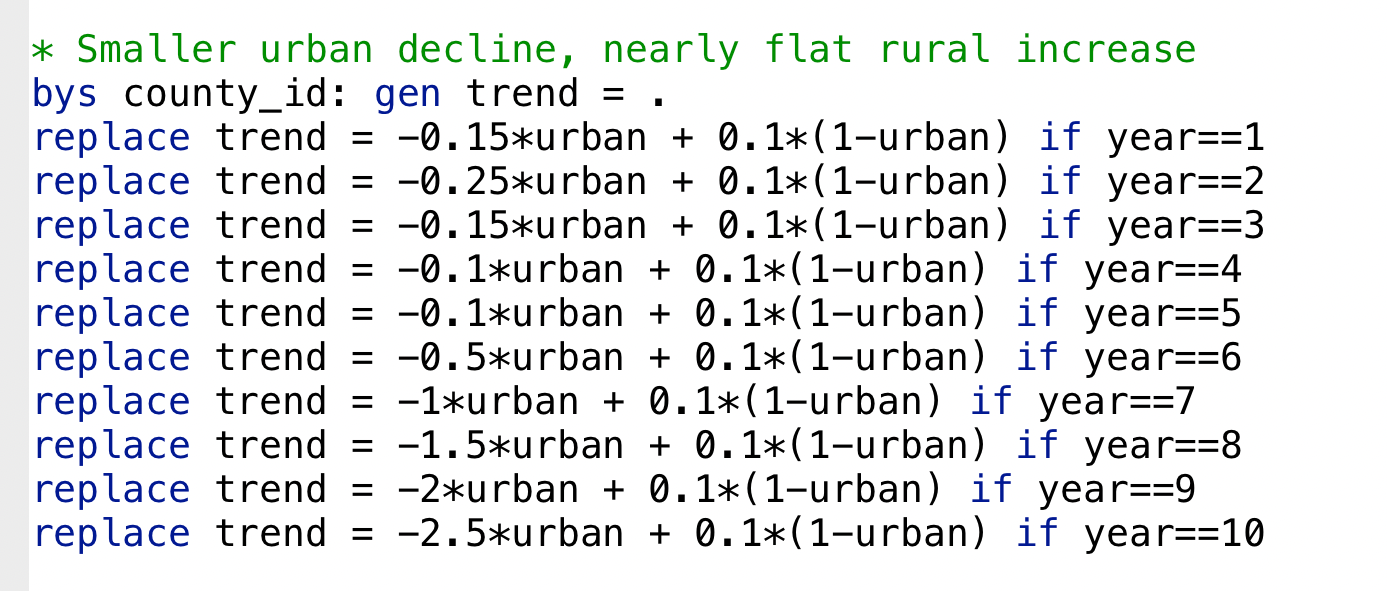
\includegraphics[width=0.6\textwidth]{./lecture_includes/covariate_trends}
\end{frame}


\begin{frame}{Assumption 5 and 6}

We need ``no X-specific trends'' for the treatment group (assumption 5) and comparison group (assumption 6)

\bigskip

\textbf{Intuition}: No X-specific trends means the evolution of potential outcome $Y^0$ is the same regardless of $X$. This would mean you cannot allow rich people to be on a different trend than poor people, for instance.

\bigskip

Without these six, in general TWFE will not identify ATT. 

\end{frame}

\begin{frame}{Why not both?}

\begin{itemize}
\item Let's review the problem.  What if you claim you need $X$ for conditional parallel trends?
\item You have three options:
	\begin{enumerate}
	\item Outcome regression (Heckman, et al. 1997) -- needs Assumptions 1-3
	\item Inverse probability weighting (Abadie 2005) -- needs Assumptions 1-3
	\item TWFE (everybody everywhere all the time) -- needs Assumptions 1-6
	\end{enumerate}
\item Problem is 1 and 2 need the models to be correctly specified
\item Let's look at a couple of Monte Carlos -- one by Pedro Sant'Anna, and then one by me
\end{itemize}

\end{frame}








\begin{frame}{Monte Carlo Simulations}

\begin{itemize}

\item First we will look at the use of these estimators using a simulation named \texttt{covariates.do} and \texttt{covariates.R}

\item We will do it both with a single run, as that's faster, and then run a simulation of 1,000 simulated regenerated data (i.e., Monte Carlo simulation) to get a distribution

\item We will examine all four estimators: (1) OLS, (2) IPW, (3) OR and (4) DR

\end{itemize}

\end{frame}

\begin{frame}{Simulation}
    \centering
    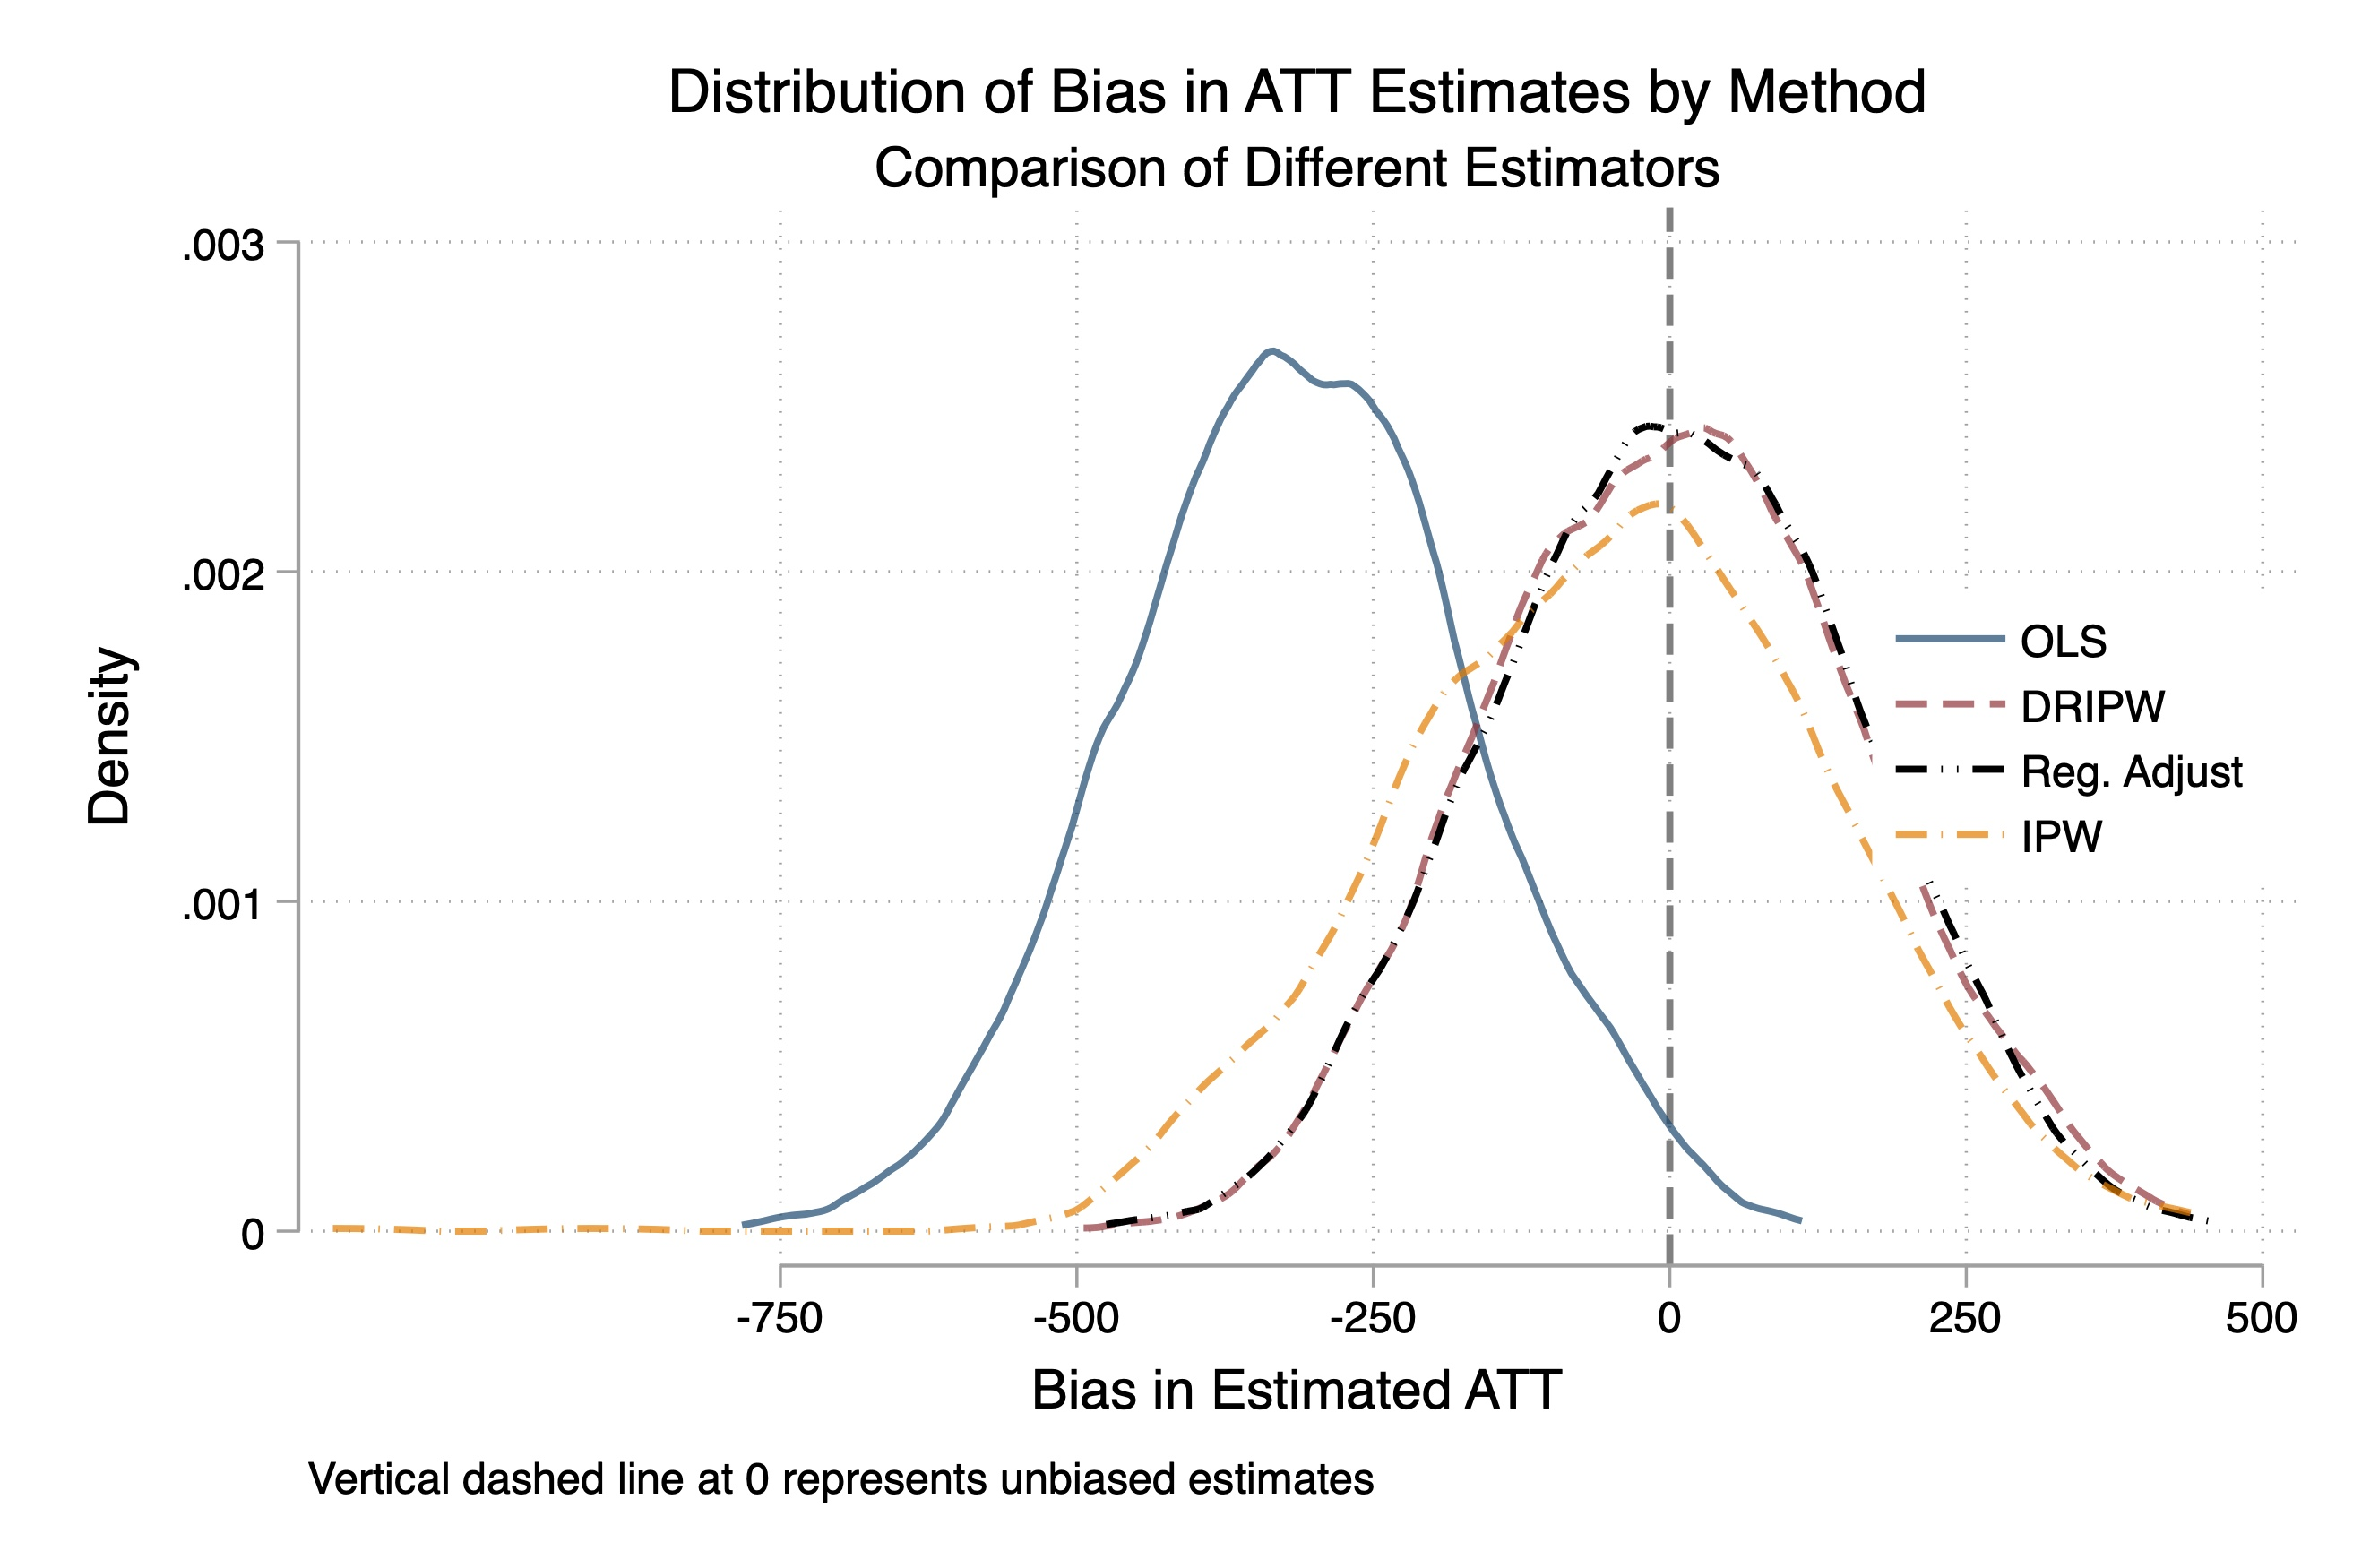
\includegraphics[width=0.6\textwidth]{./lecture_includes/covariates.jpg}
\end{frame}

\begin{frame}{Real world example of questionable unconditional parallel trends}

\begin{itemize}
\item Me, Christine Durrance, and Melanie Guldi have been working on a project for years looking at online dating's effect on birth rates
	\begin{itemize}
	\item Thickening of relationship markets
	\item Reduced search costs
	\item Formation of better relationships meant for forming families
	\end{itemize}
\item But online dating companies have an incentive to perpetuate dating despite claims to the contrary, which may reduce the formation of families
\item Plus so many confounders -- websites appeared simultaneously, smart phones, social media, and birth rates plummeted after Great Recession ("demographic transition")
\end{itemize}
\end{frame}





\begin{frame}

\begin{figure}
    \centering
    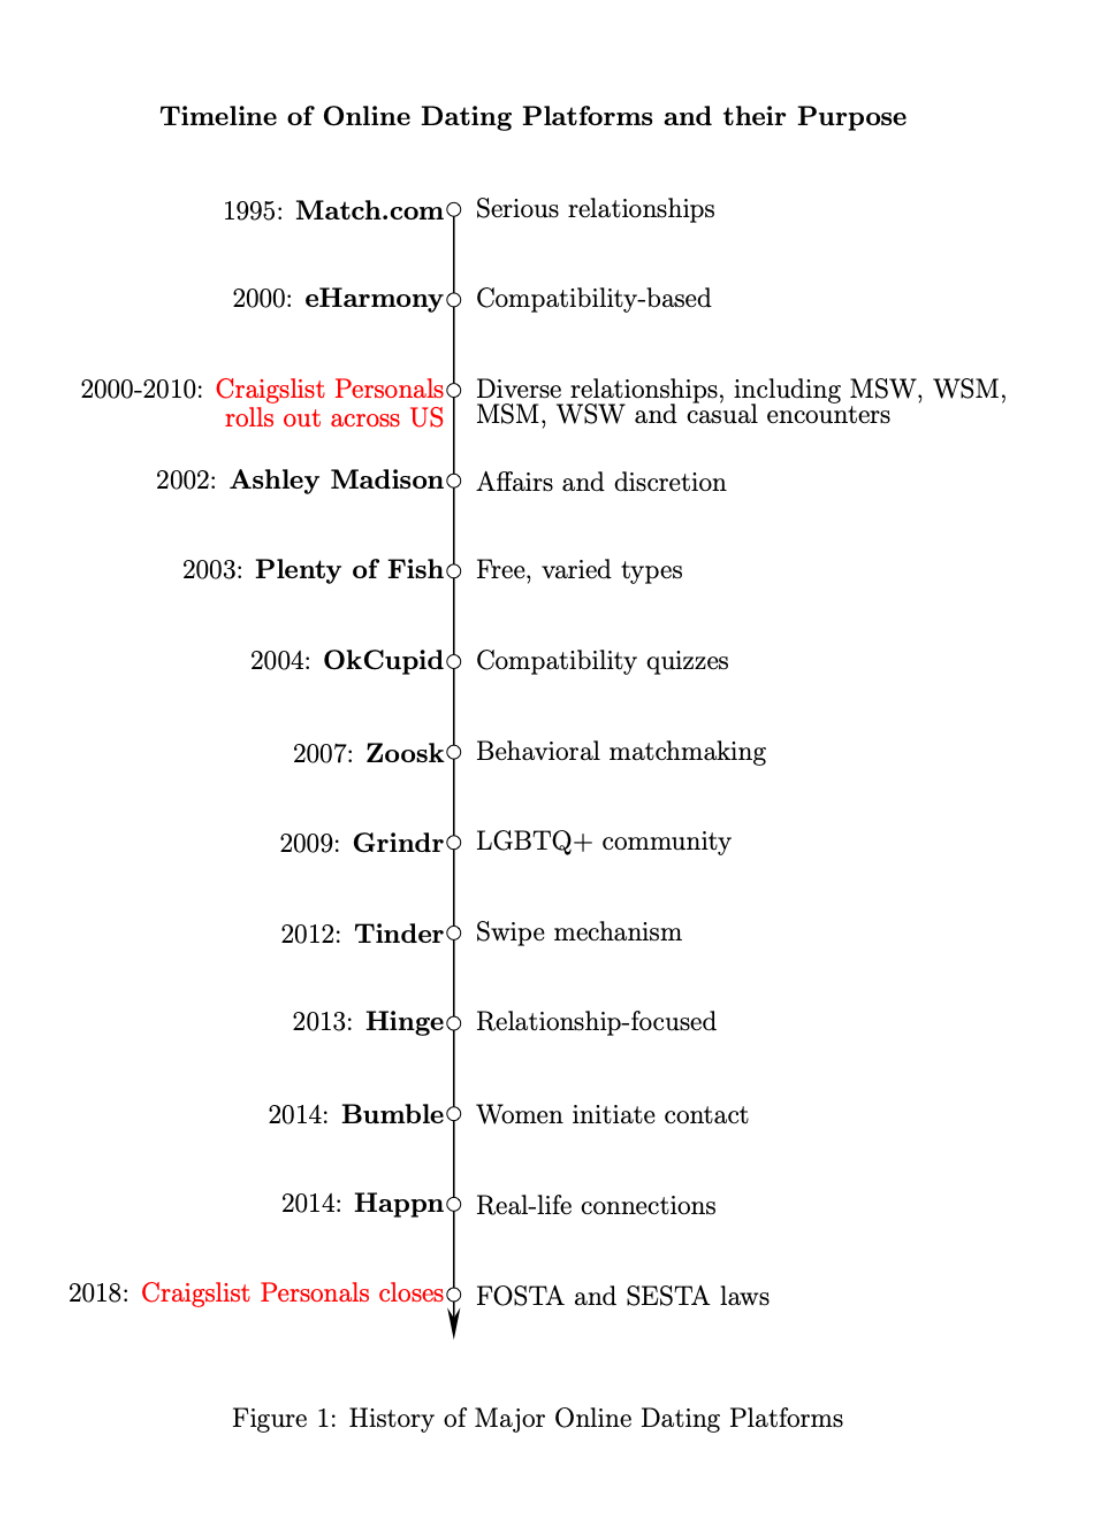
\includegraphics[height=0.95\textheight]{./lecture_includes/craigslist_online}
\end{figure}

\end{frame}



\begin{frame}

\begin{figure}
    \centering
    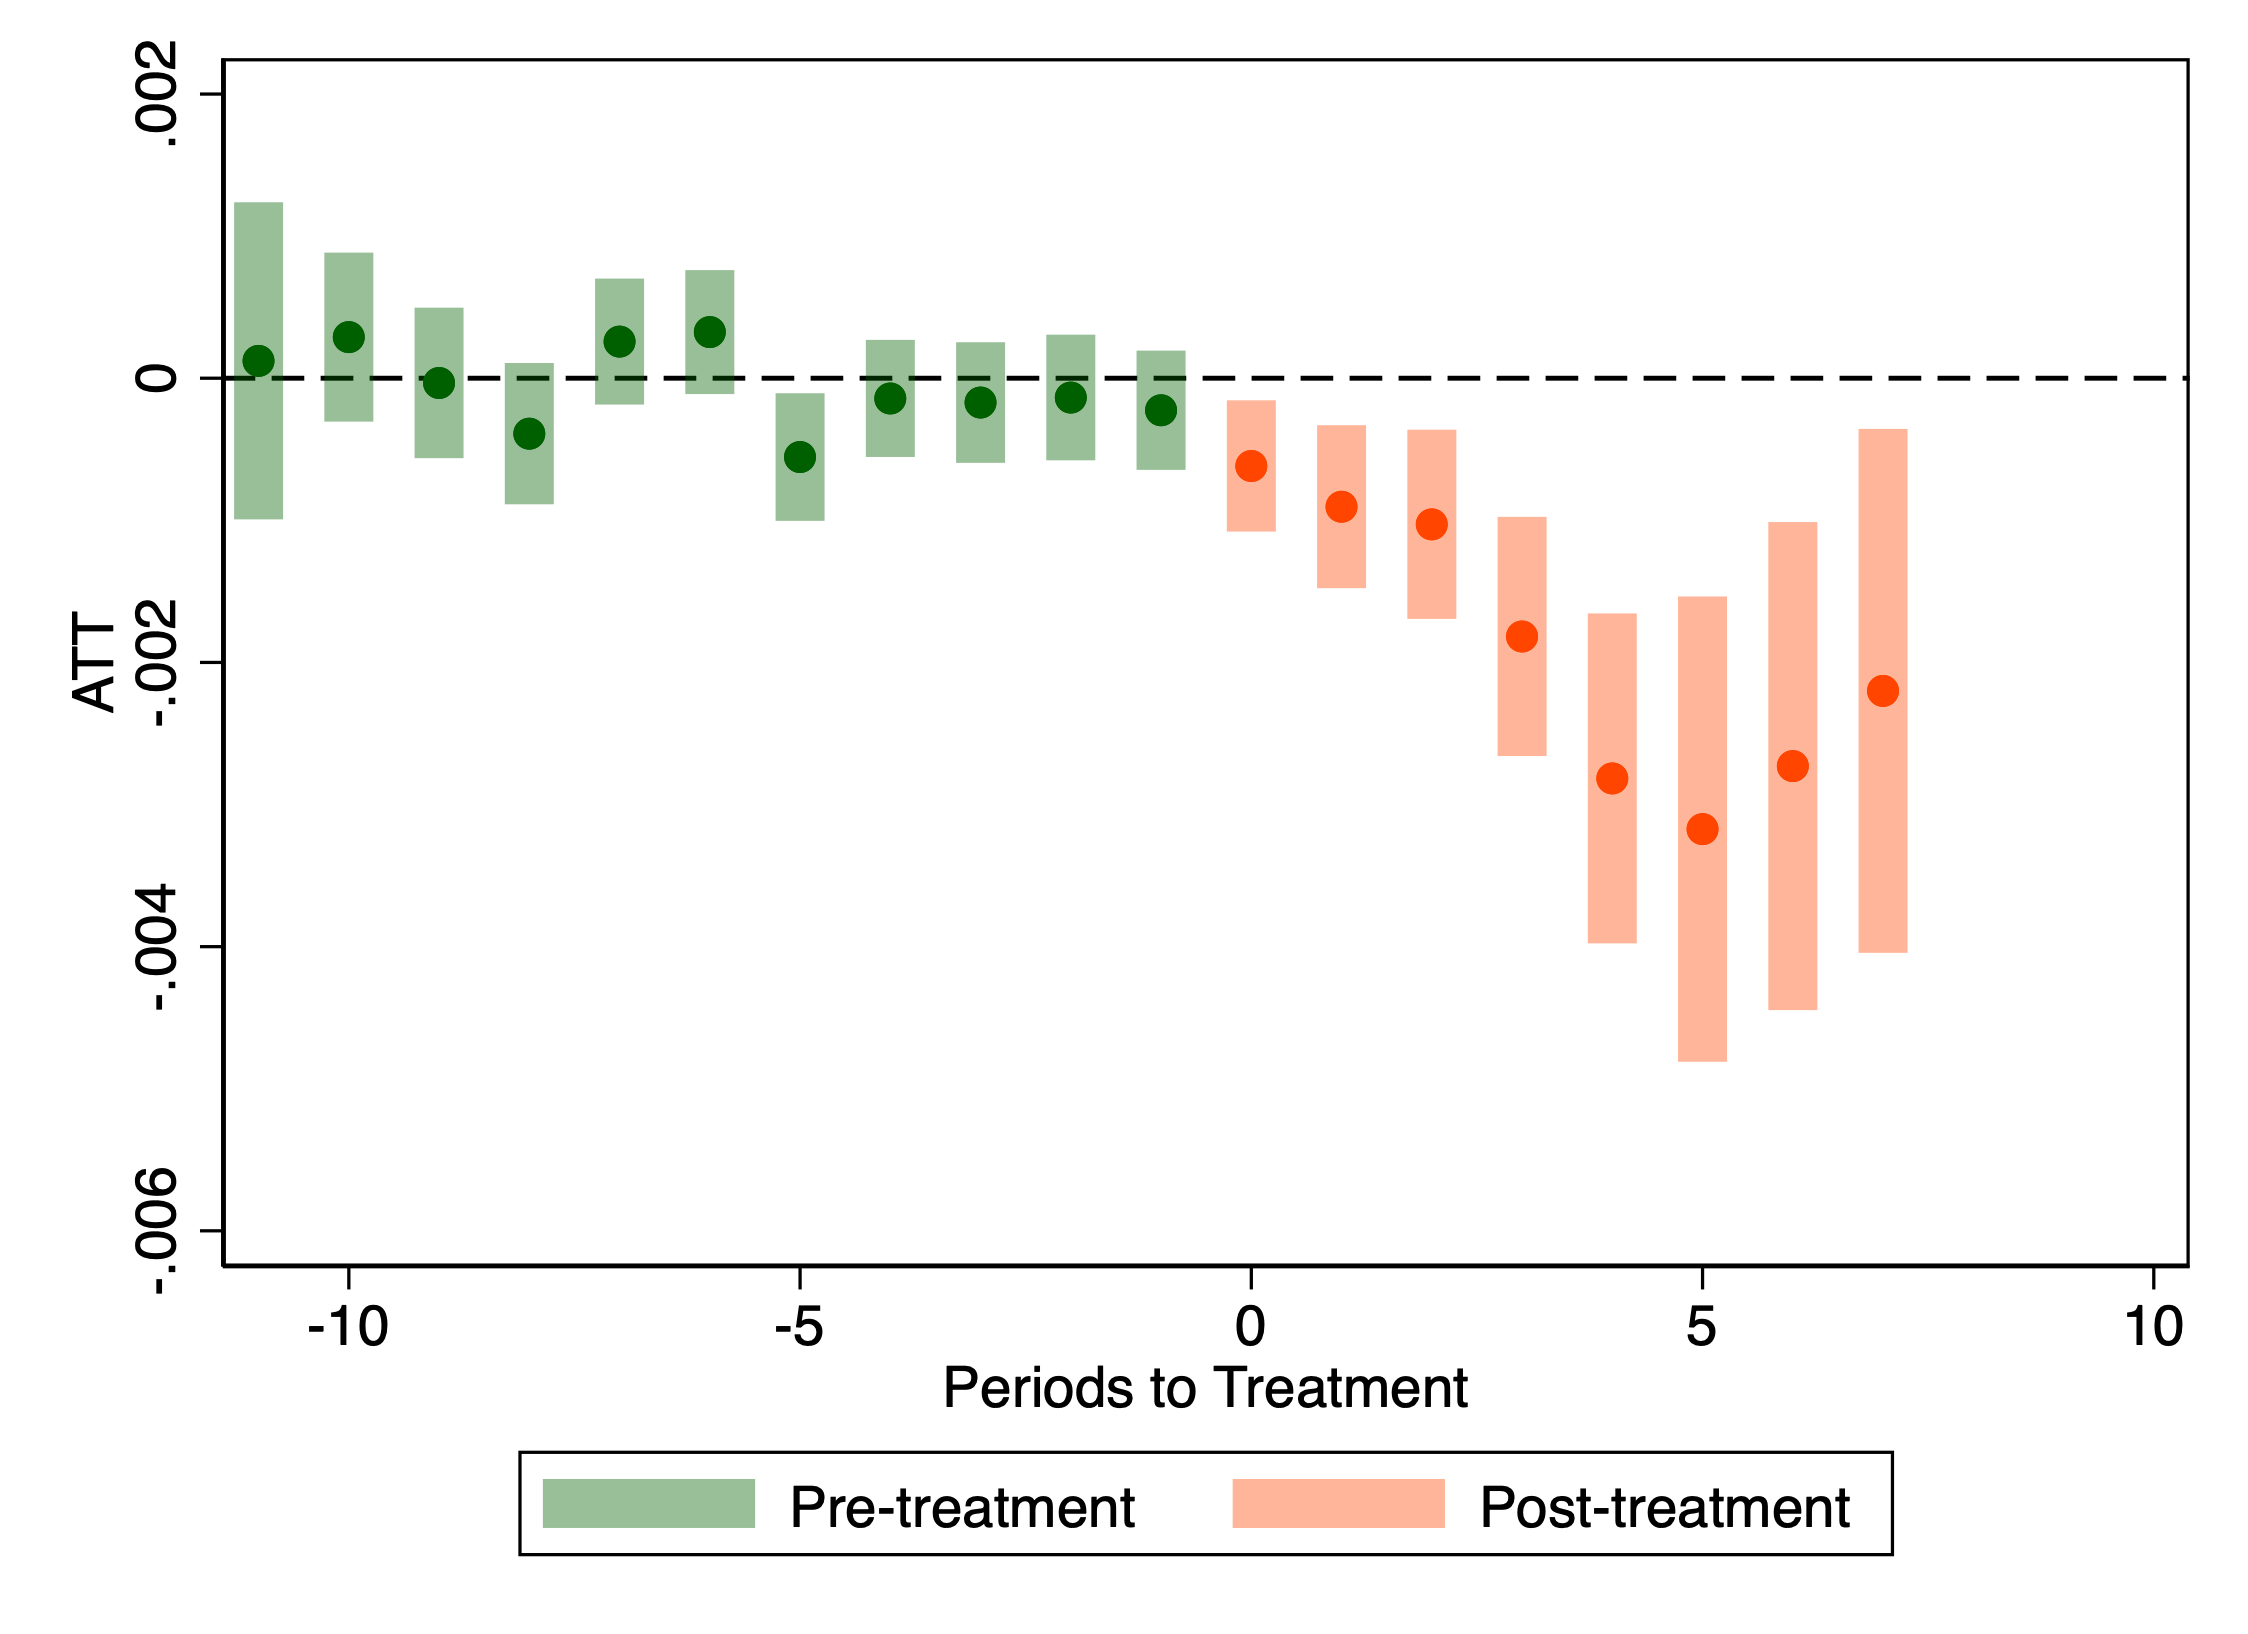
\includegraphics[height=0.85\textheight]{./lecture_includes/es_br1544_shortgap.png}
\end{figure}

\end{frame}


\begin{frame}{Scrutinizing that event study}

\begin{itemize}
\item There are two things going on in that graph
	\begin{enumerate}
	\item Notice the decline in coefficients leading into $t-1$ as opposed to $t-1$ being a solid circle -- called "short gap" calculation of event study coefficients, which is possible with new estimators but impossible with regressions
	\item No covariates
	\end{enumerate}
\item We are comparing each period to the period to its left, but OLS used the $t-1$ as its baseline
\item Plus without controlling for covariates, we are assuming that ordinarily, small and large counties would have evolved similarly, but we know sorting into large vs small counties is not random
\end{itemize}
\end{frame}

\begin{frame}{Scrutinizing that event study}

\begin{itemize}
\item So we do two things: 
	\begin{enumerate}
	\item We use the same method as OLS for calculating the event studies ("long difference"), 
	\item We include a control for how urban the county is with a 9-digit variable (RUCC)
	\end{enumerate}
\item Compare the first event study to the last one, and see if you can spot the difference 
\end{itemize}
\end{frame}

\begin{frame}{Short Gap vs. Long Difference}

\begin{figure}[htbp]
    \centering
    \begin{minipage}[b]{0.48\textwidth}
        \centering
        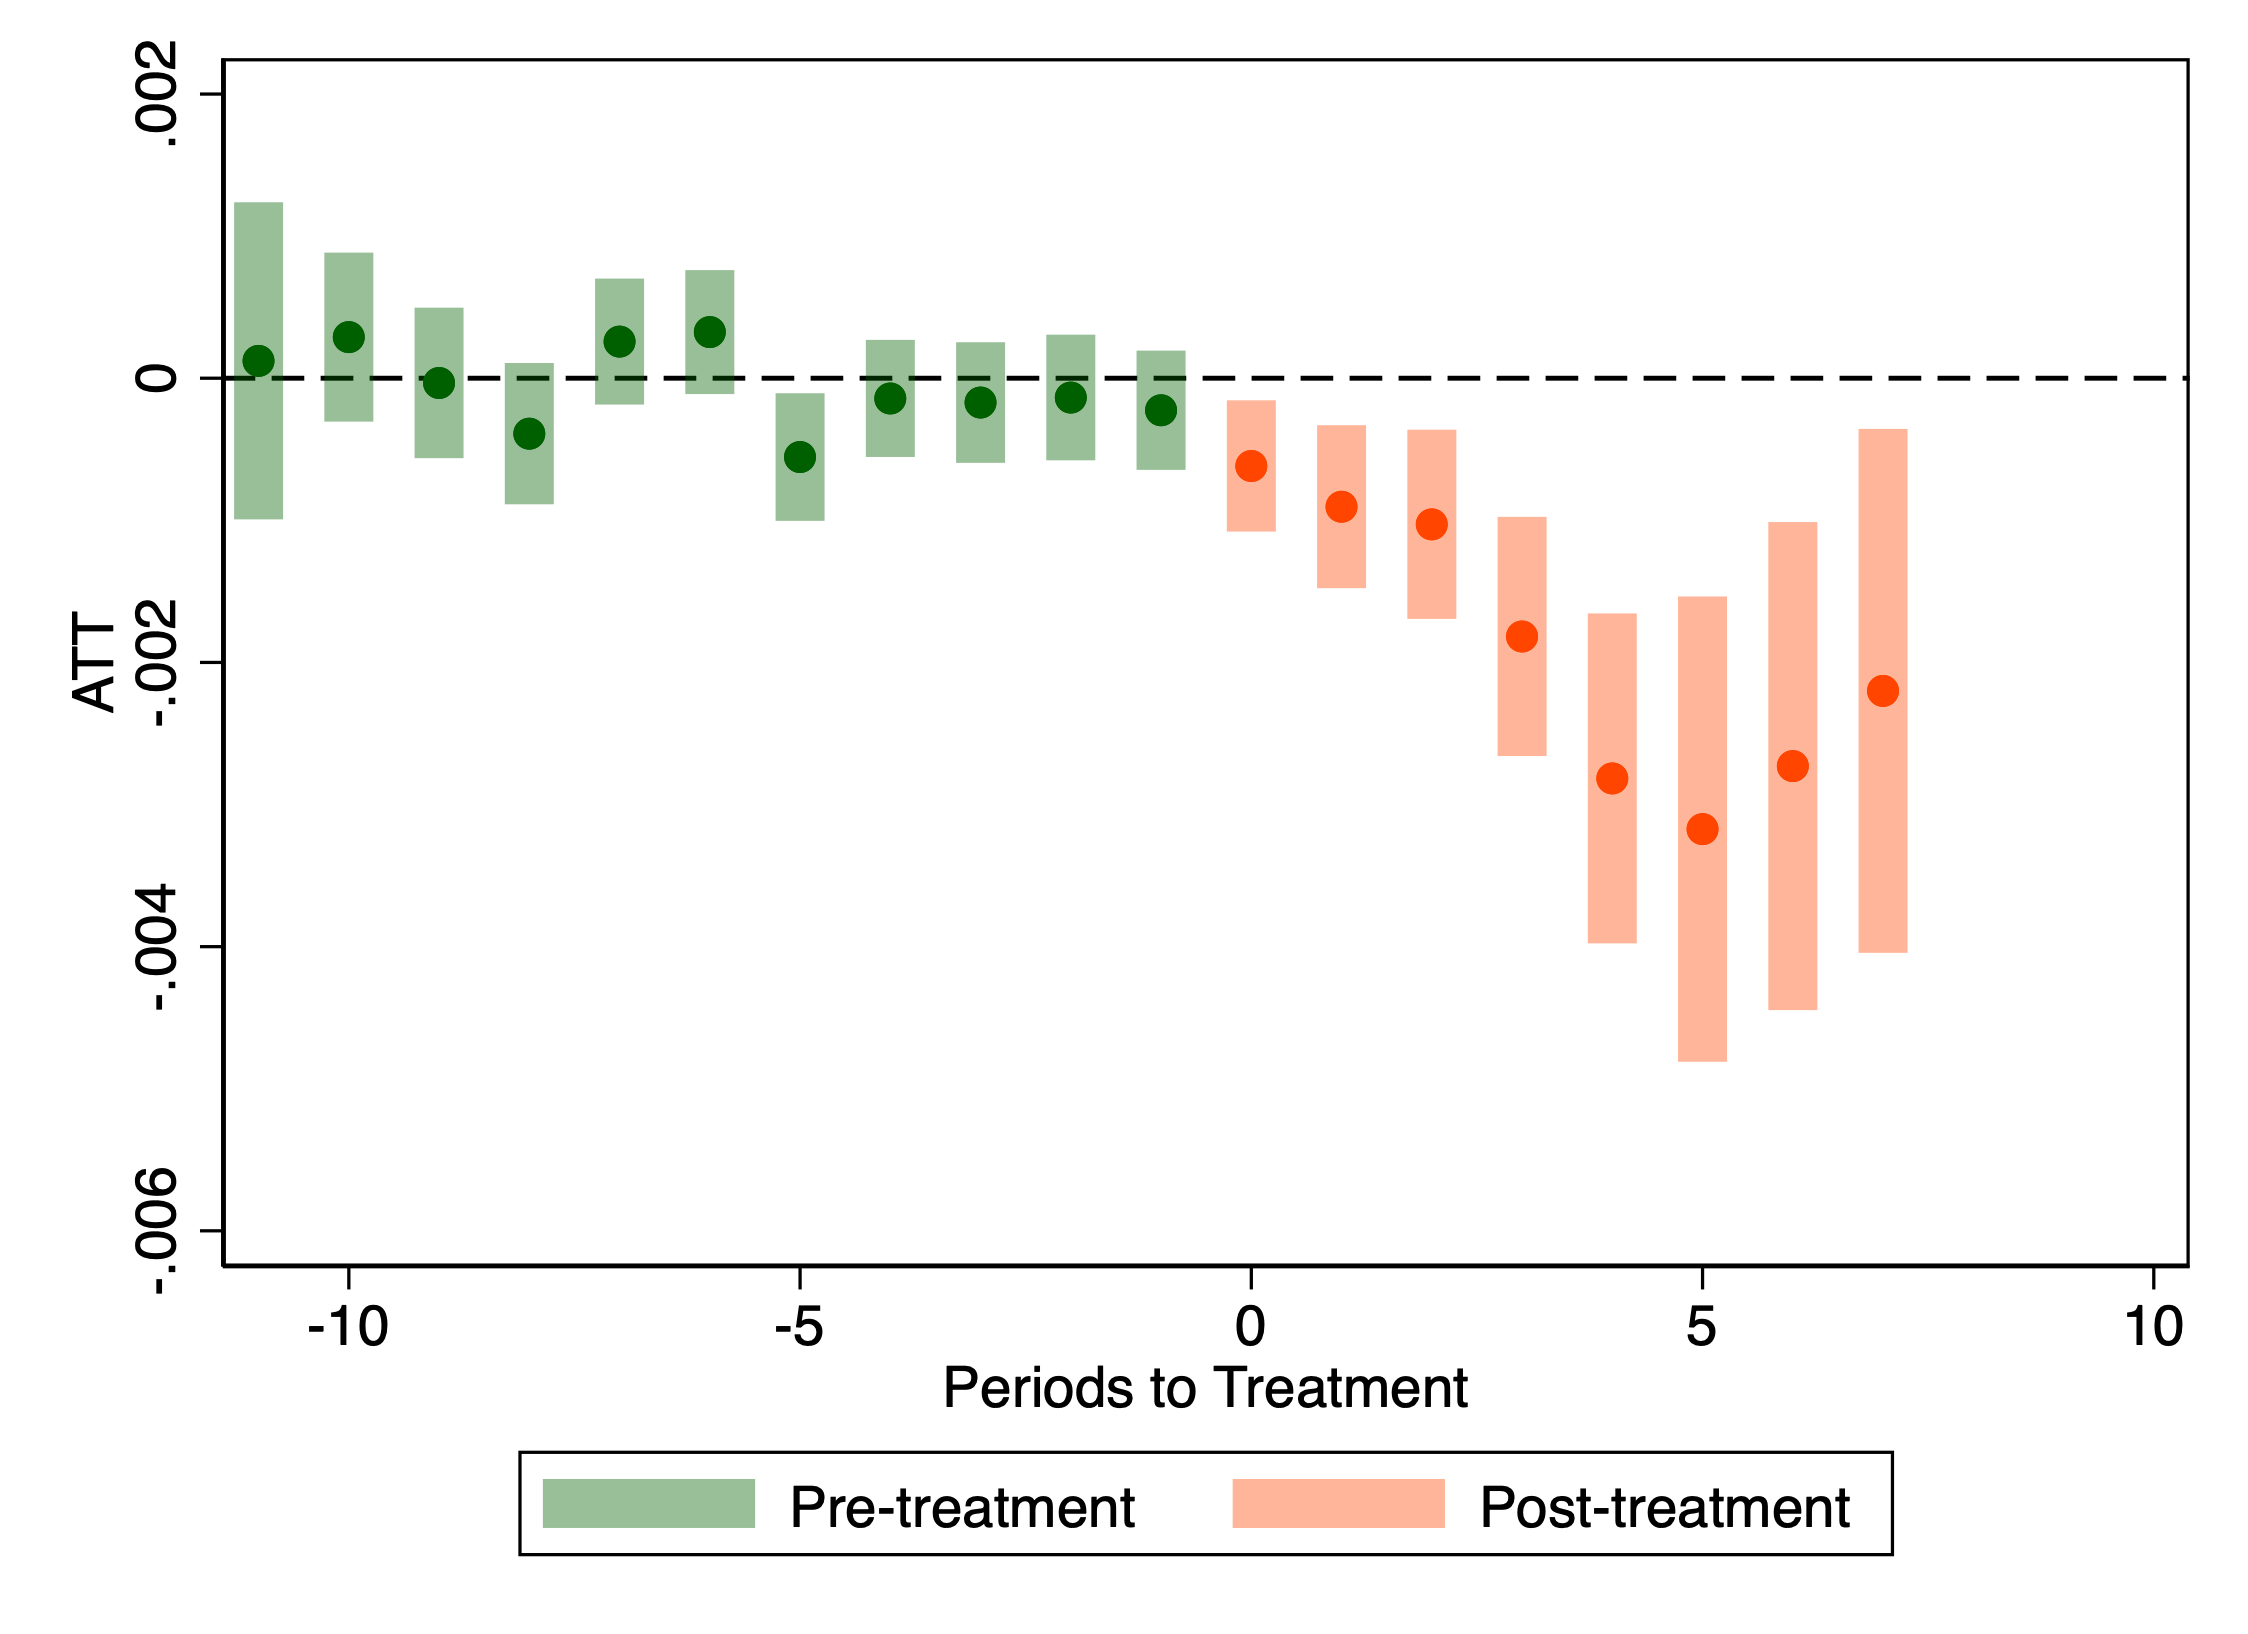
\includegraphics[width=\textwidth,height=0.75\textheight,keepaspectratio]{./lecture_includes/es_br1544_shortgap.png}
        \caption{Short Gap}
    \end{minipage}
    \hfill
    \begin{minipage}[b]{0.48\textwidth}
        \centering
        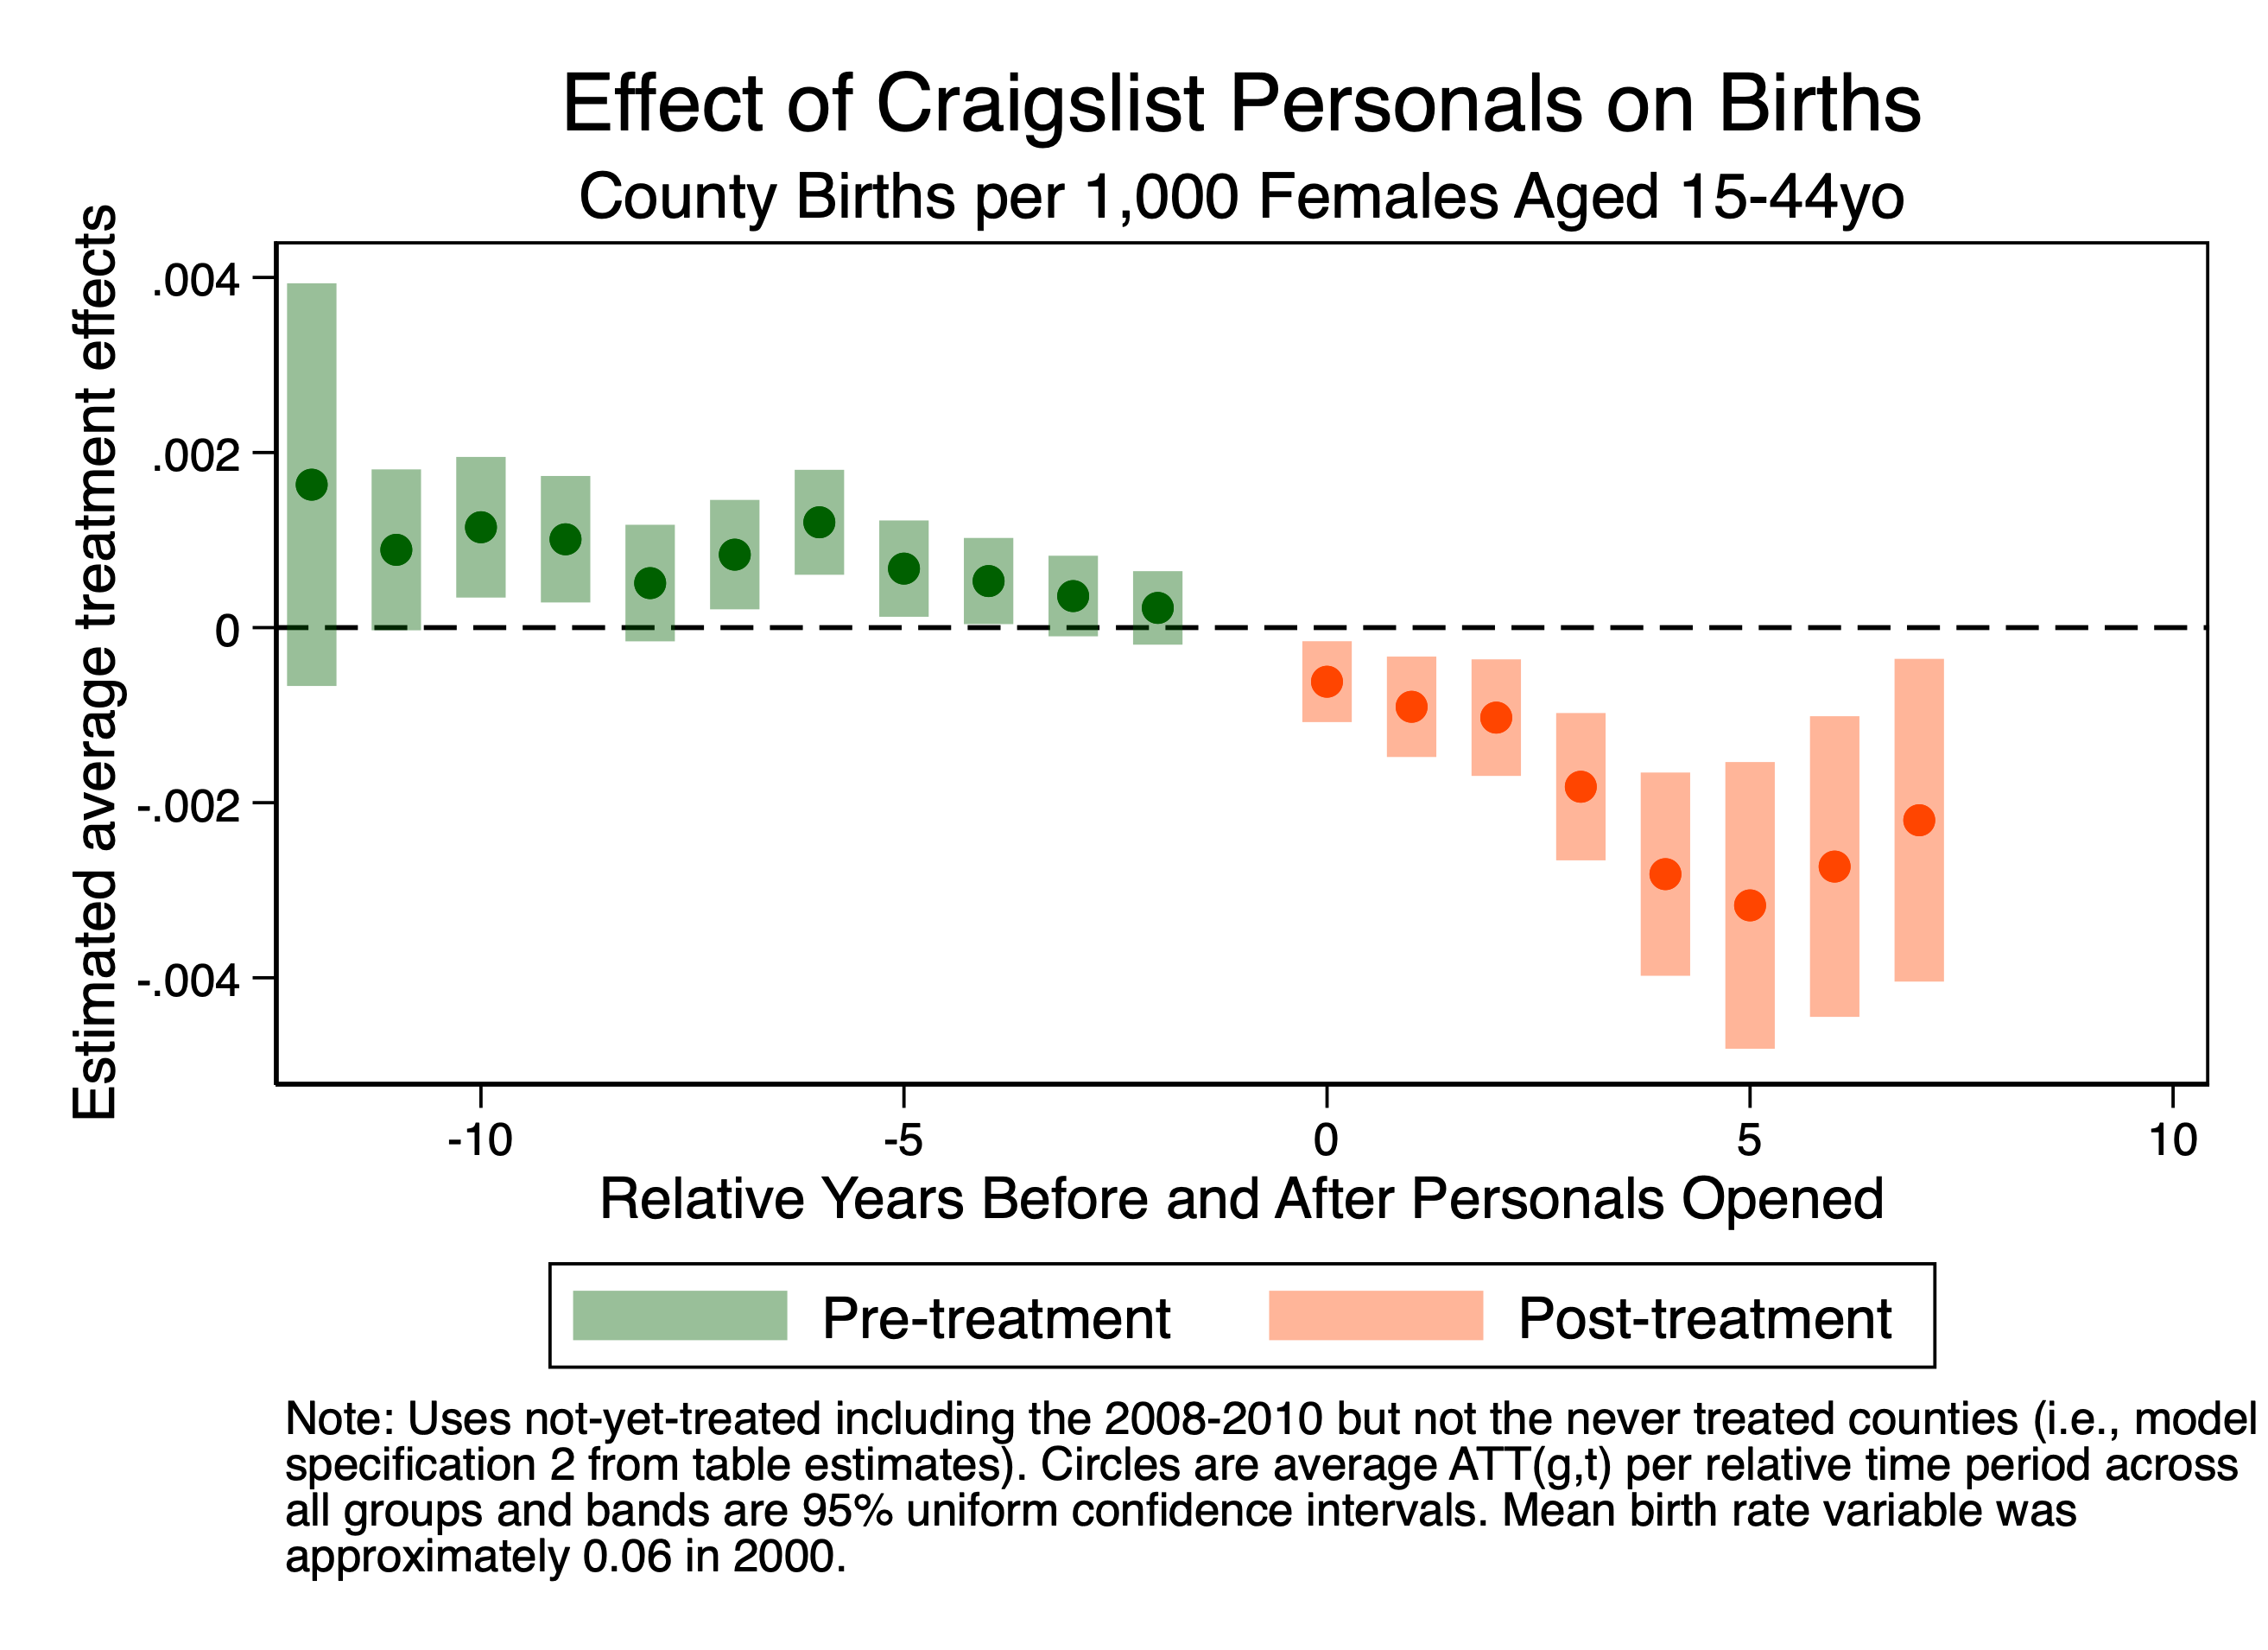
\includegraphics[width=\textwidth,height=0.75\textheight,keepaspectratio]{./lecture_includes/es_births2.png}
        \caption{Long Difference}
    \end{minipage}
\end{figure}

\pause

\begin{itemize}
\item Question 1: how could you have seen that the event study was "short gap" vs "long difference"? \pause
\item Question 2: What is the relationship between the negative coefficients under short gap and the positive coefficients in long difference?
\end{itemize}

\end{frame}

\begin{frame}{Is Unconditional parallel trends plausible?}

\begin{itemize}
\item Without covariates, we are explicitly assuming that the treatment and control group would have evolved similarly in birth rates
\item But what if Craigslist entered certain kinds of counties differently than others?
\item What if the ones it entered earlier had different birth rate trends?
\item Let's look at the rollout by urban status
\end{itemize}

\end{frame}

\begin{frame}{Small numbers are more urban}

\begin{figure}
    \centering
    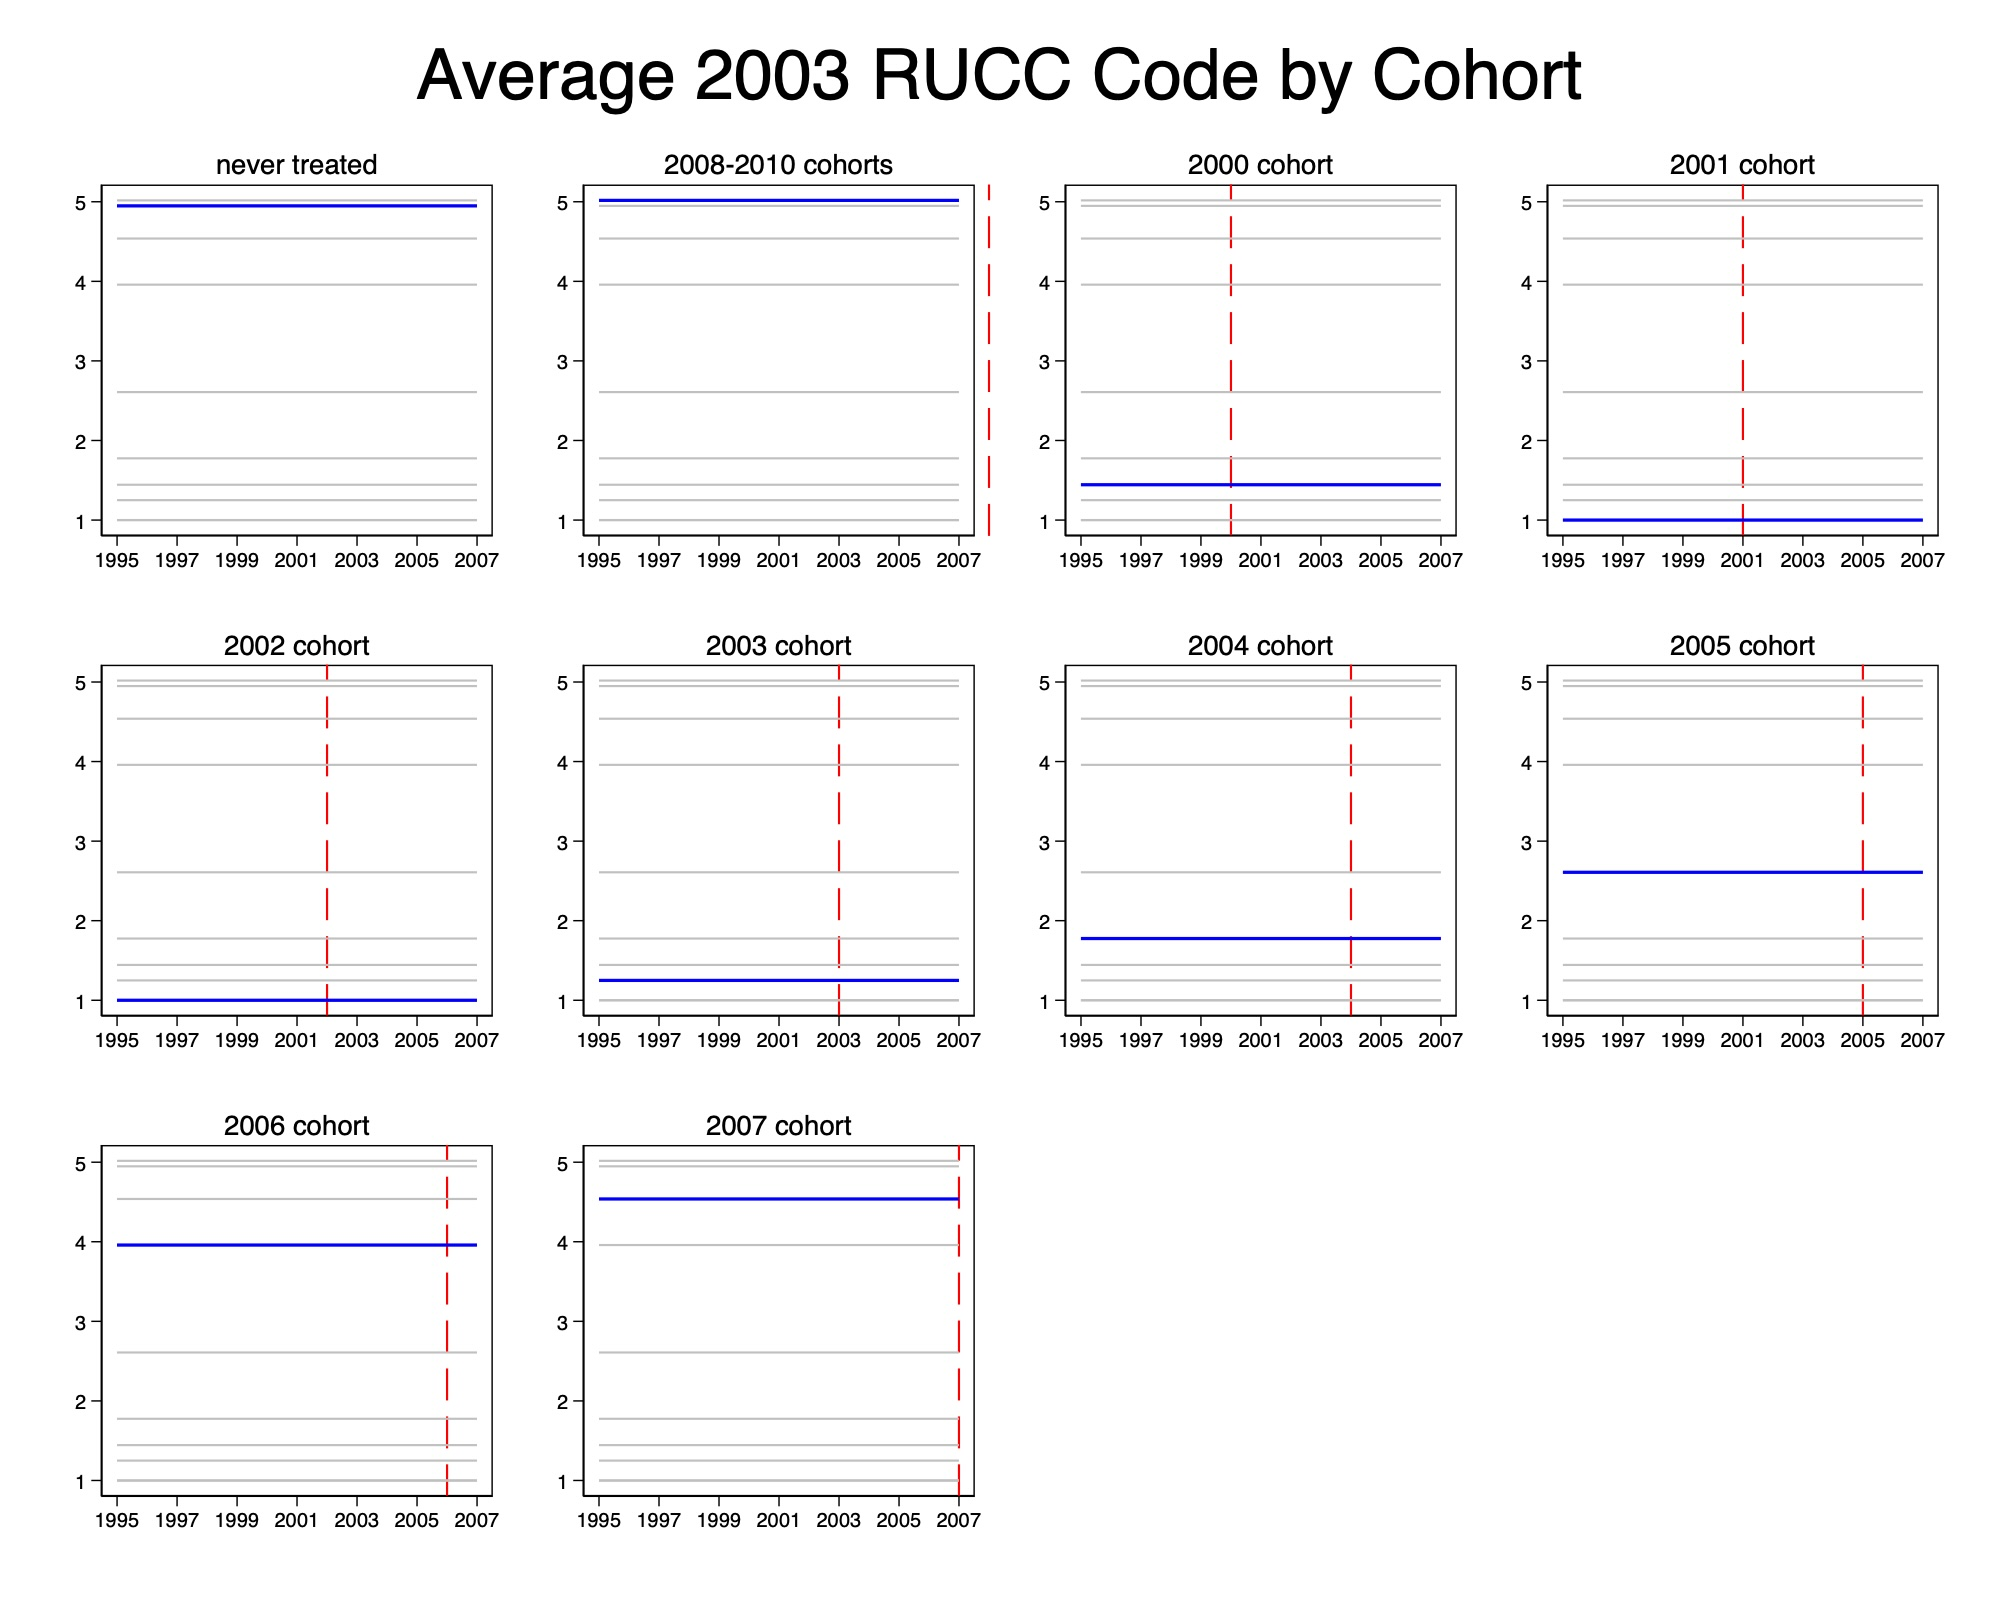
\includegraphics[height=0.85\textheight]{./lecture_includes/pretty_RUCC}
\end{figure}

\end{frame}






\begin{frame}

\begin{figure}
    \centering
    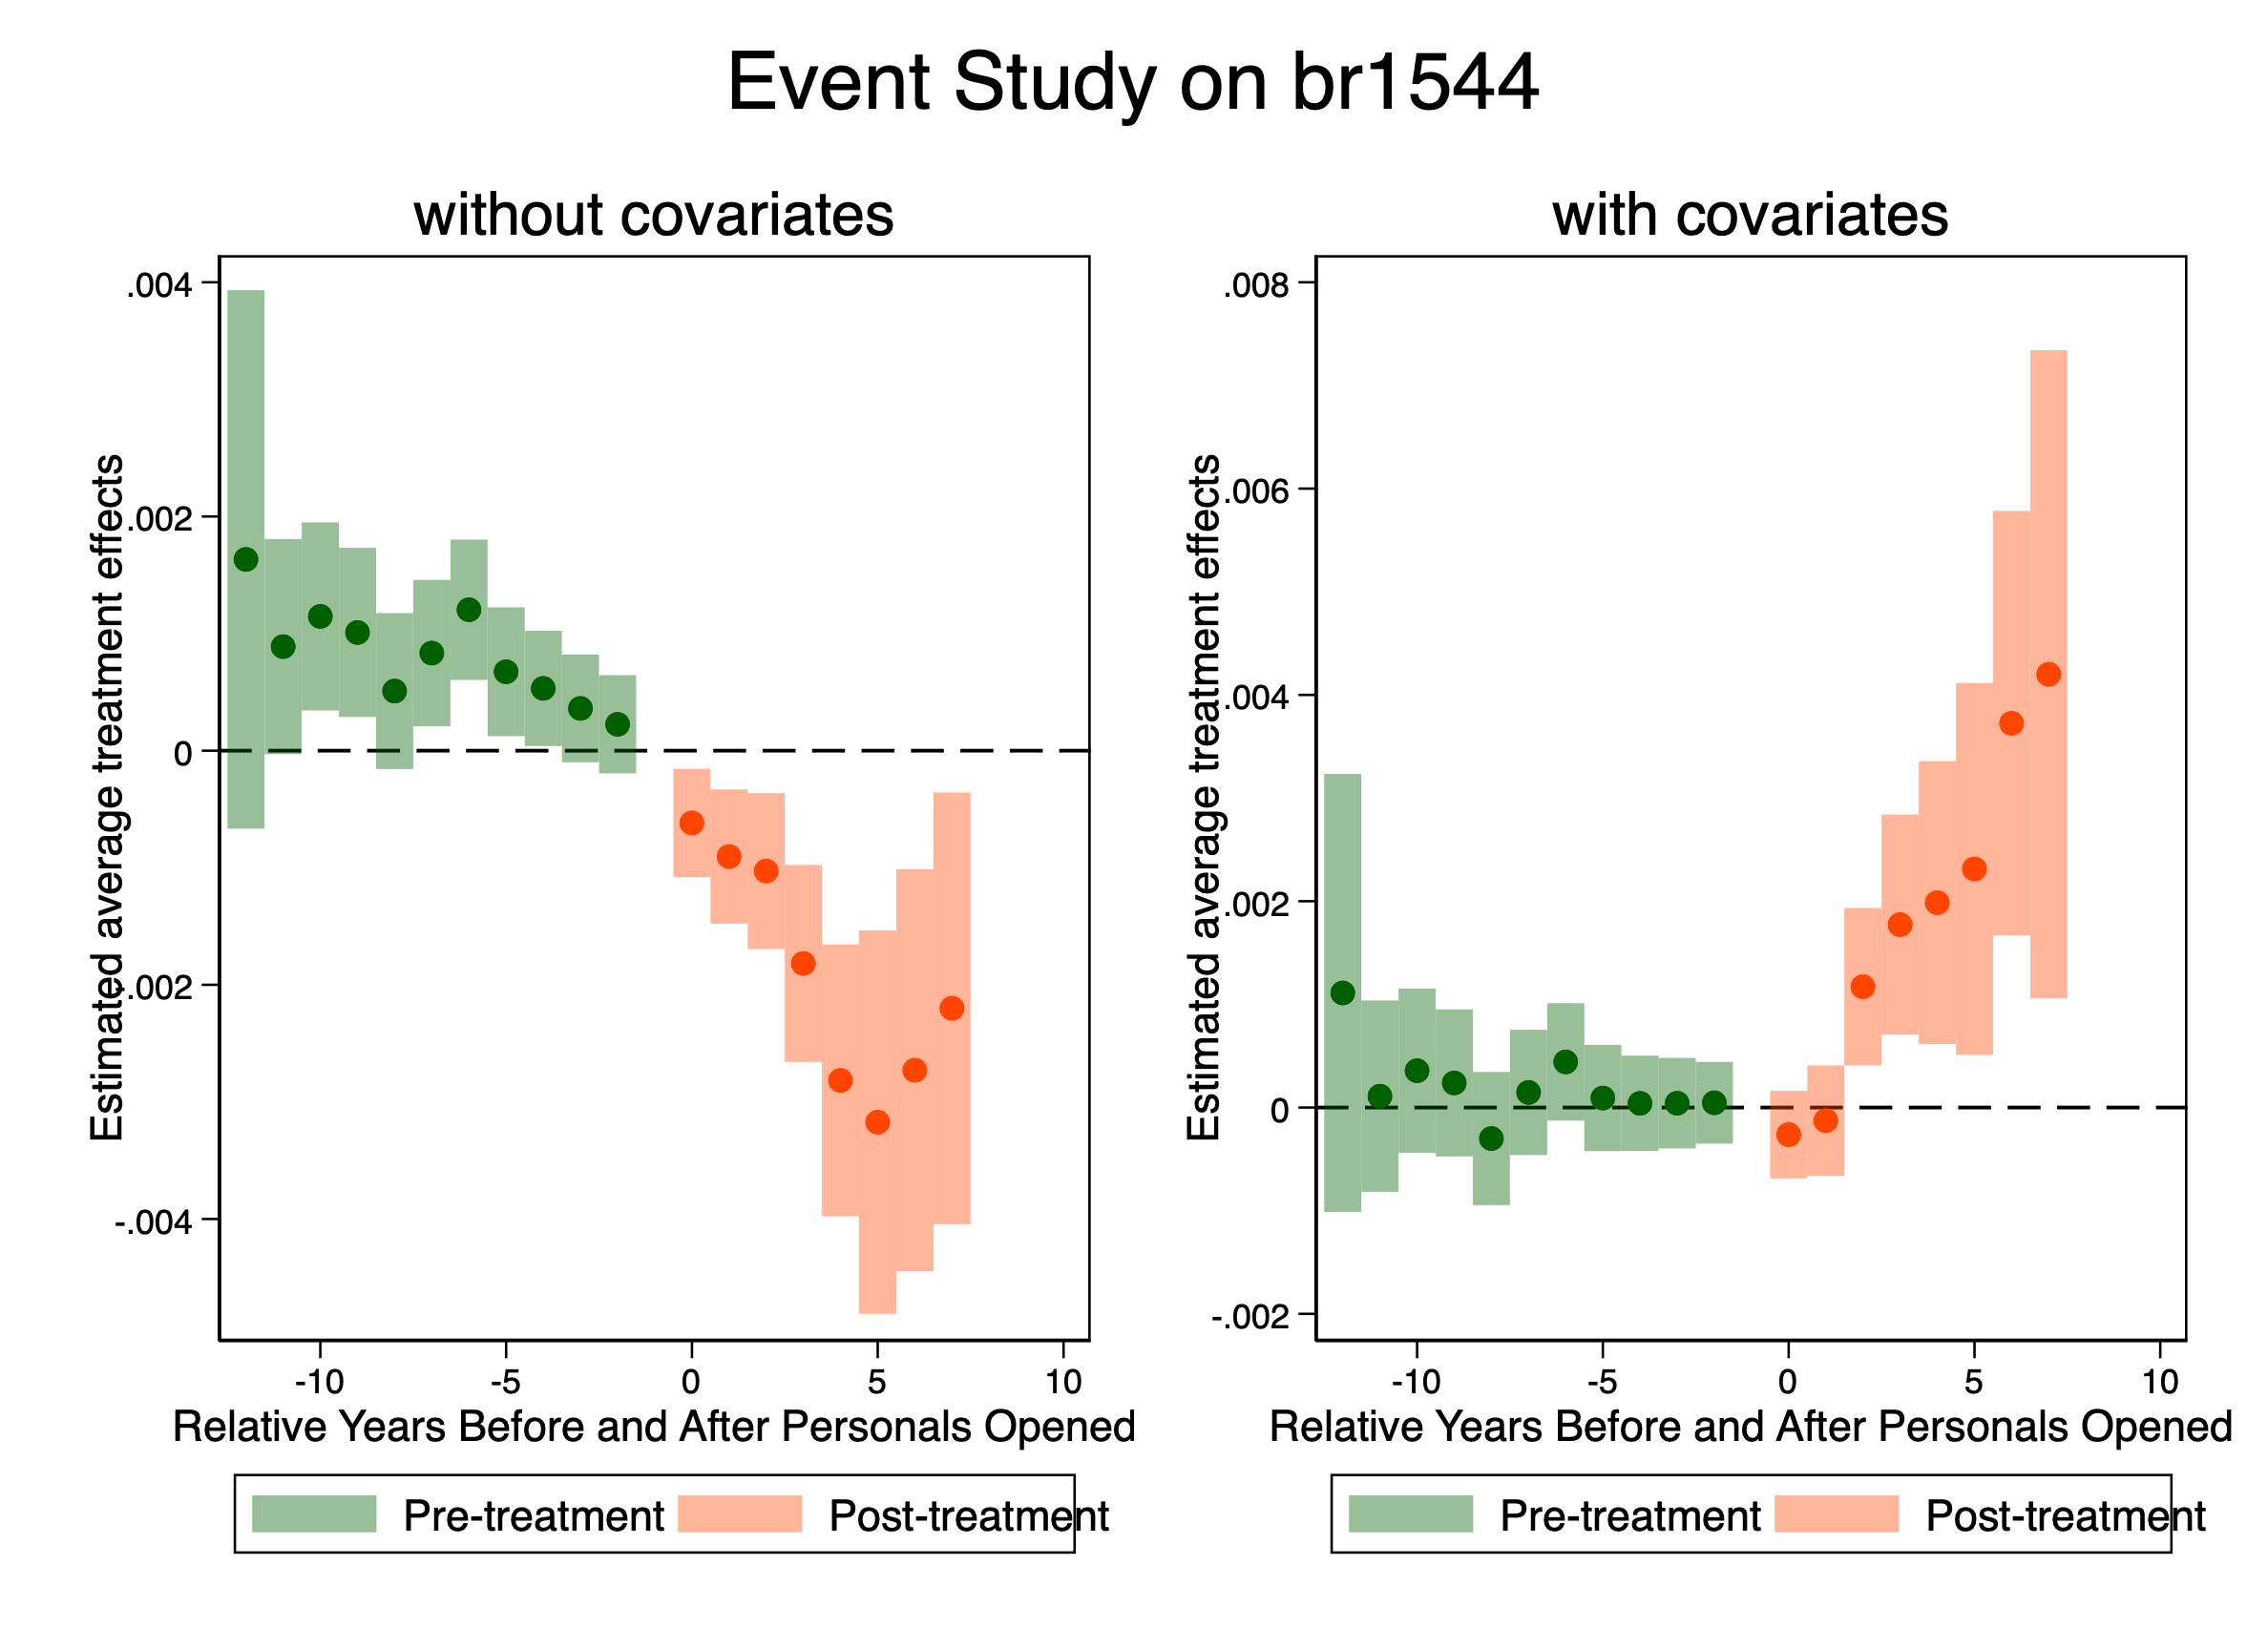
\includegraphics[height=0.95\textheight]{./lecture_includes/es_br1544_combined.png}
\end{figure}

\end{frame}

\begin{frame}{Shoeleather and DiD}

\begin{itemize}

\item Do everything you can to understand selection -- shoeleather dominates technical knowledge (Rubin 2008 "Design Trumps Analysis"; Freedman 1991)
\item John Snow did not just download data and run regressions -- he worked hard to find comparable groups, learn the institutional details, and think carefully about selection
\item Do everything you can to figure out the treatment assignment mechanism 
\item Consider interviewing key people!
\end{itemize}

\end{frame}

\begin{frame}[shrink=20]
    \centering
    \begin{center}
    \begin{figure}
        
\includegraphics[width=\textwidth]{./lecture_includes/craig_dm}
    \end{figure}
    \end{center}
    
    \vspace{0.5cm} % Add some space between the image and the text

    
\end{frame}



\begin{frame}{What happened?}

\begin{itemize}
\item What happened?  Craigslist tended to target urban counties so treatment were highly urban and control highly rural
\item Remember that what's missing in the ATT is $\textcolor{red}{E[Y^0|D=1]}$ and we use the control group trends in its $Y^0$ to \emph{impute} the missing $\textcolor{red}{E[Y^0|D=1]}$
\item It's actually pretty basic -- do you think cities have different birth rate trends than counties?  If so, then that imputation is likely to be bad
\item But what if you imputed $Y^0$ apples for apples -- use cities in the control to impute cities in the treatment

\end{itemize}
\end{frame}








\begin{frame}{Event studies can mislead}

\begin{itemize}

\item People mistakenly equate parallel trends with parallel pretrends, but you can have one without the other, both or neither
\item One of the ways you can have parallel pre-trends but violate parallel trends is if the trends change differentially by covariate over time (called x-specific trends)
\item Code is called \texttt{misleading_eventstudy.do} and \texttt{misleading_eventstudy.R}
\item Note how well the unconditional parallel trends assumption appears to be when reviewing the graphs only
\end{itemize}

\end{frame}

\begin{frame}{Event studies can mislead}

\begin{figure}
    \centering
    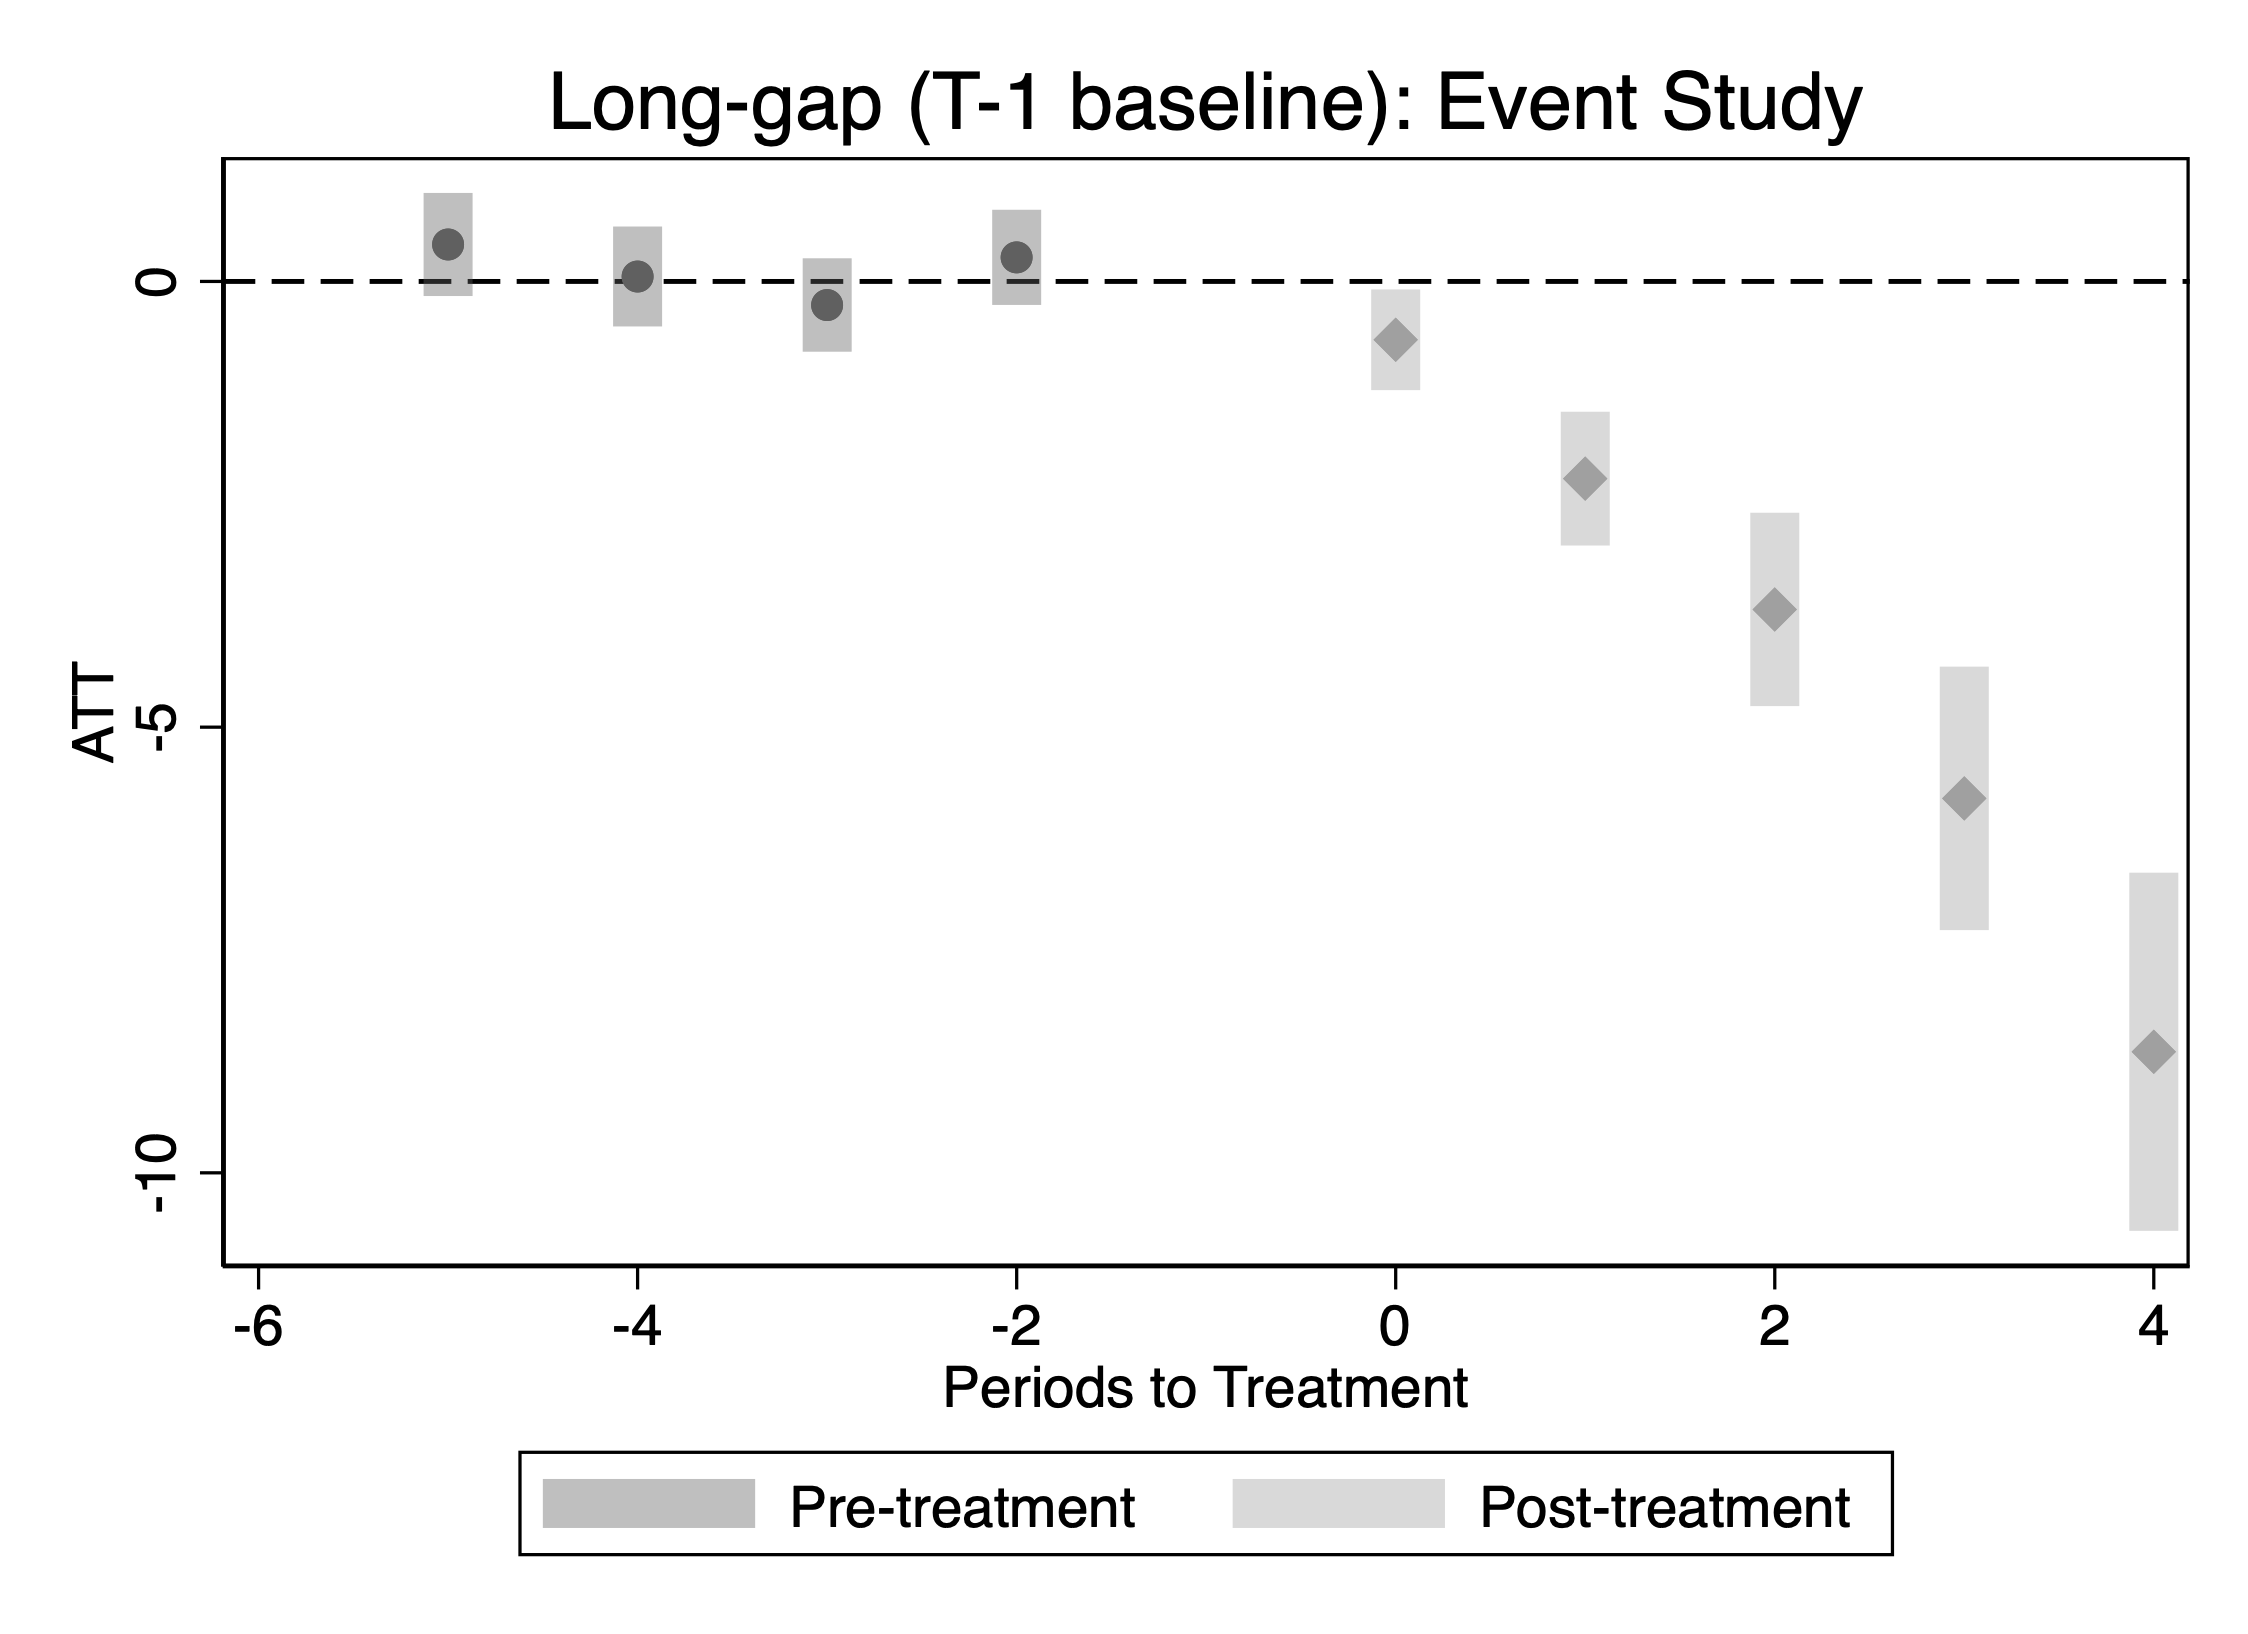
\includegraphics[height=0.75\textheight]{./lecture_includes/es_flawed.png}
\end{figure}

\end{frame}


\begin{frame}{Event studies can mislead}

\begin{figure}
    \centering
    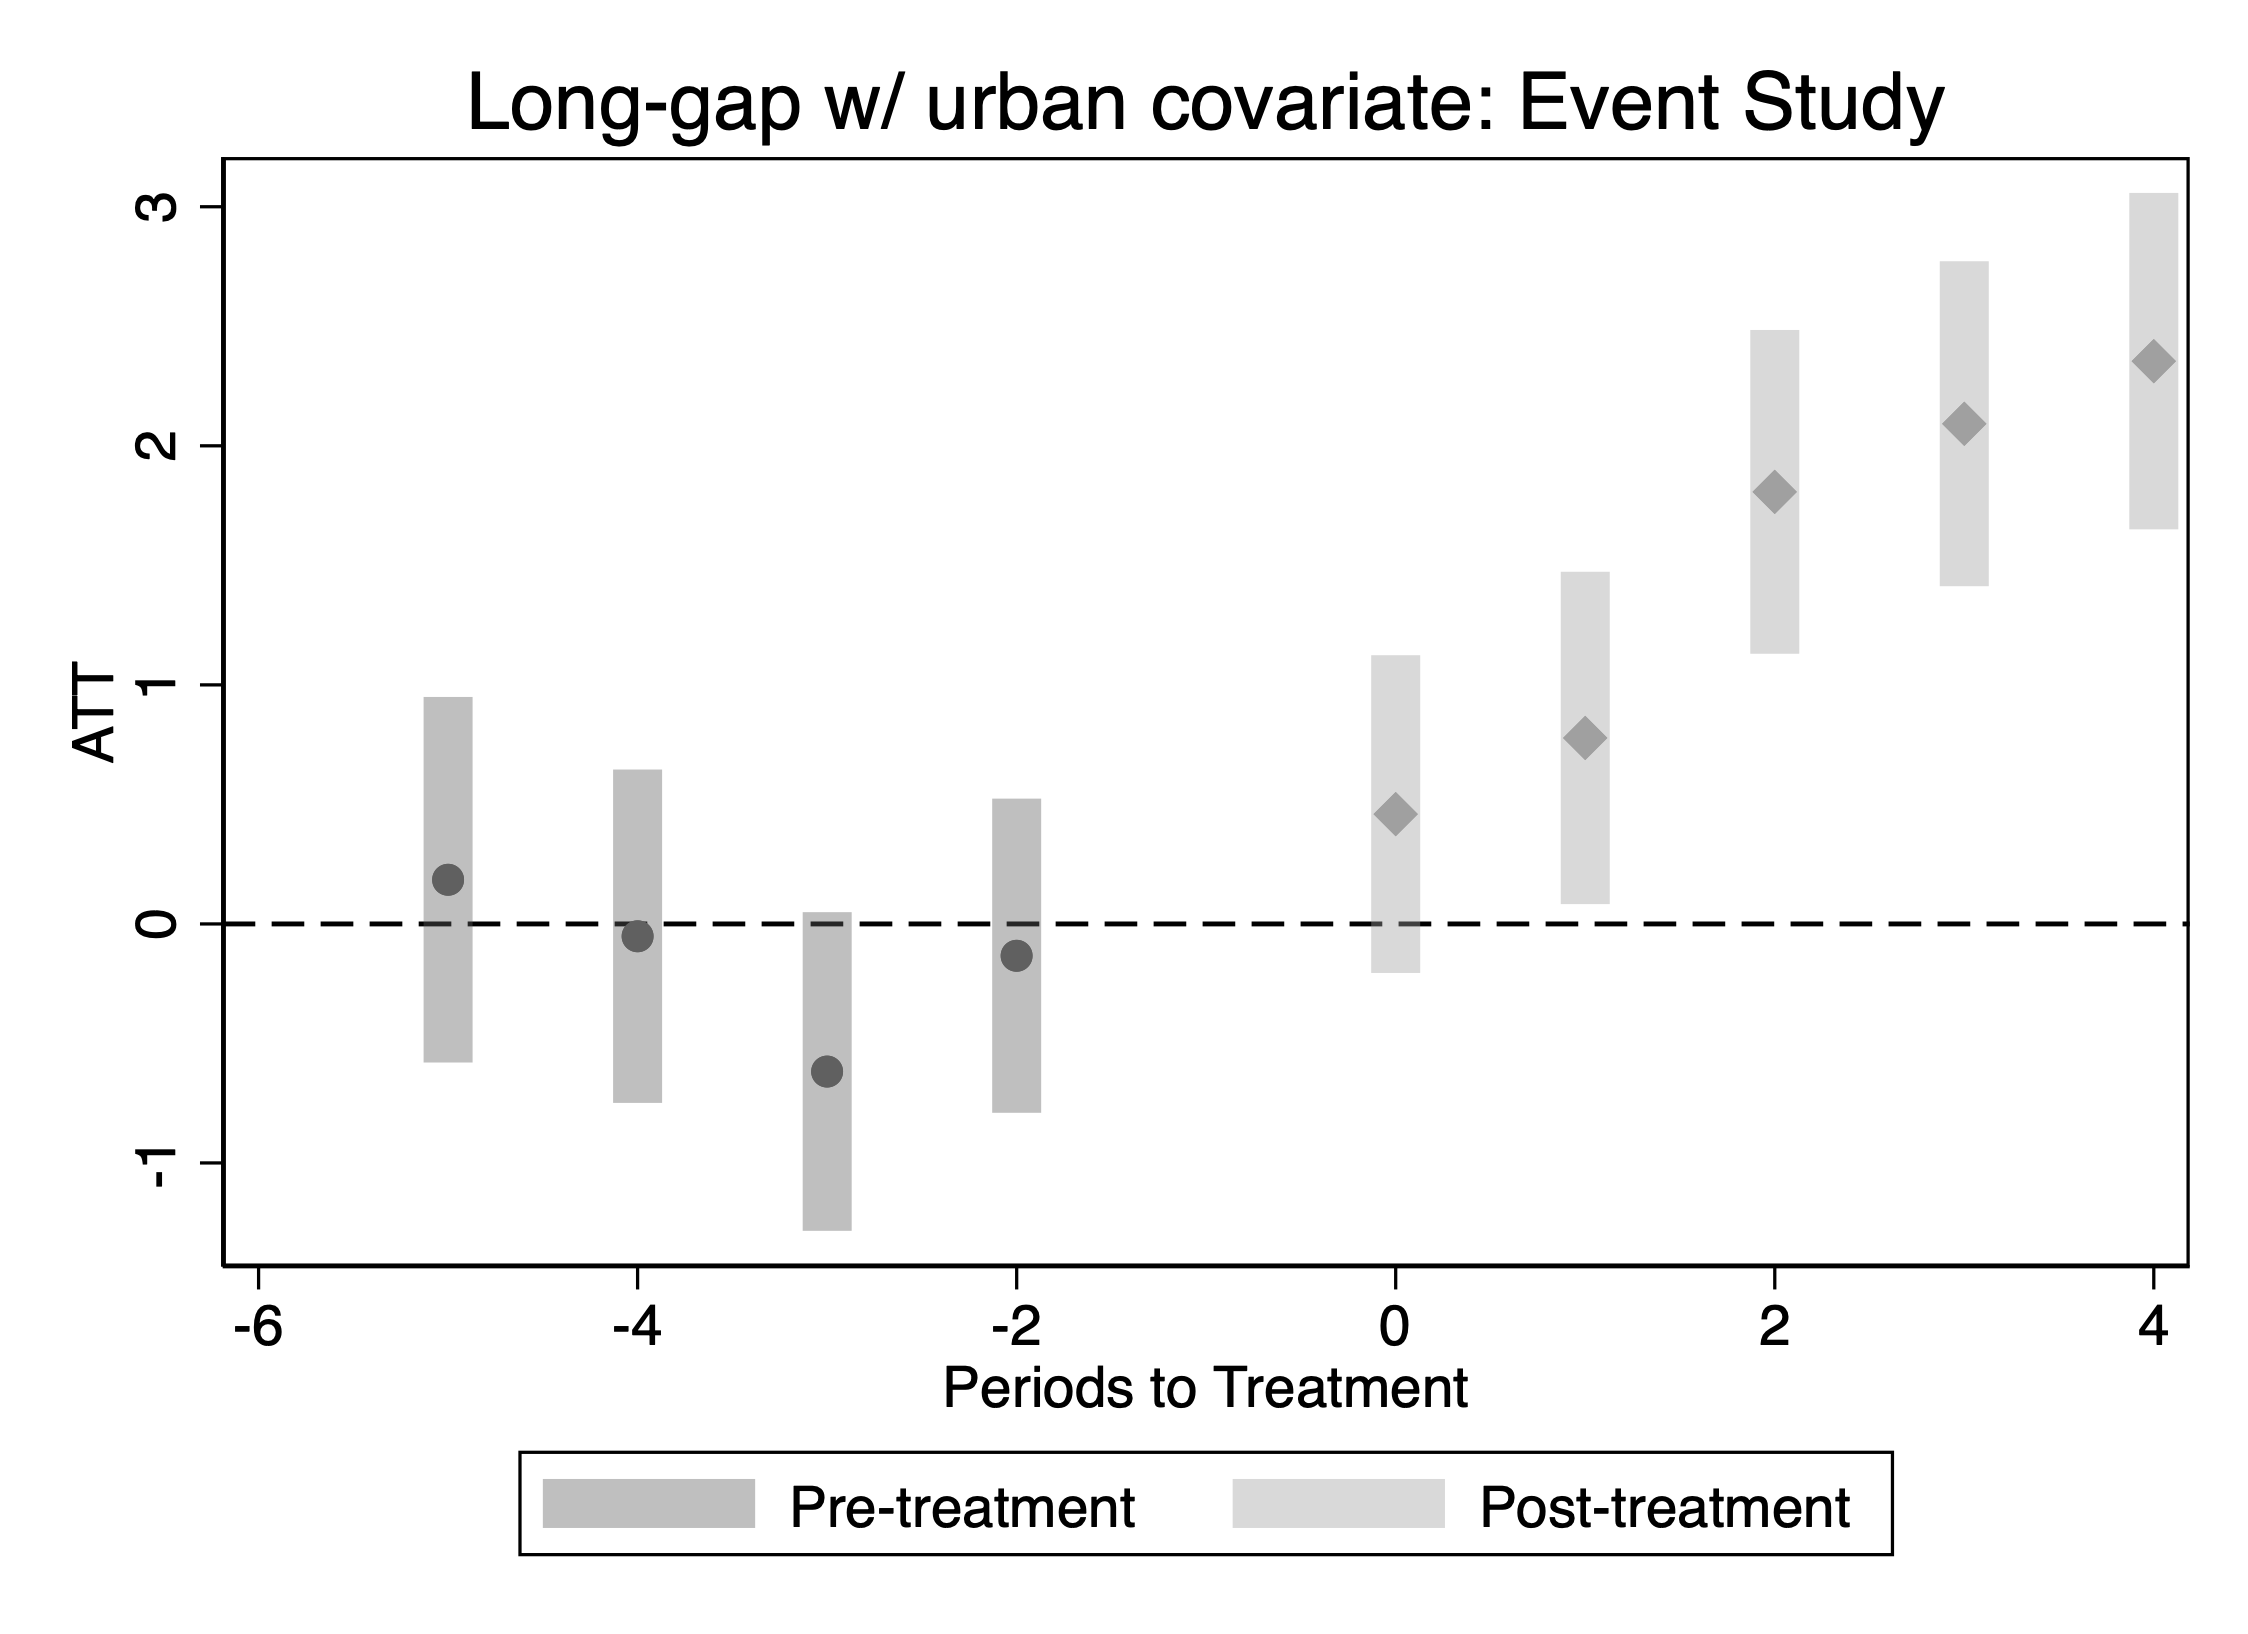
\includegraphics[height=0.75\textheight]{./lecture_includes/es_correct.png}
\end{figure}

\end{frame}

\begin{frame}{Time varying trends in $Y^0$ have \emph{nothing} to do with parallel trends}

\begin{figure}
    \centering
    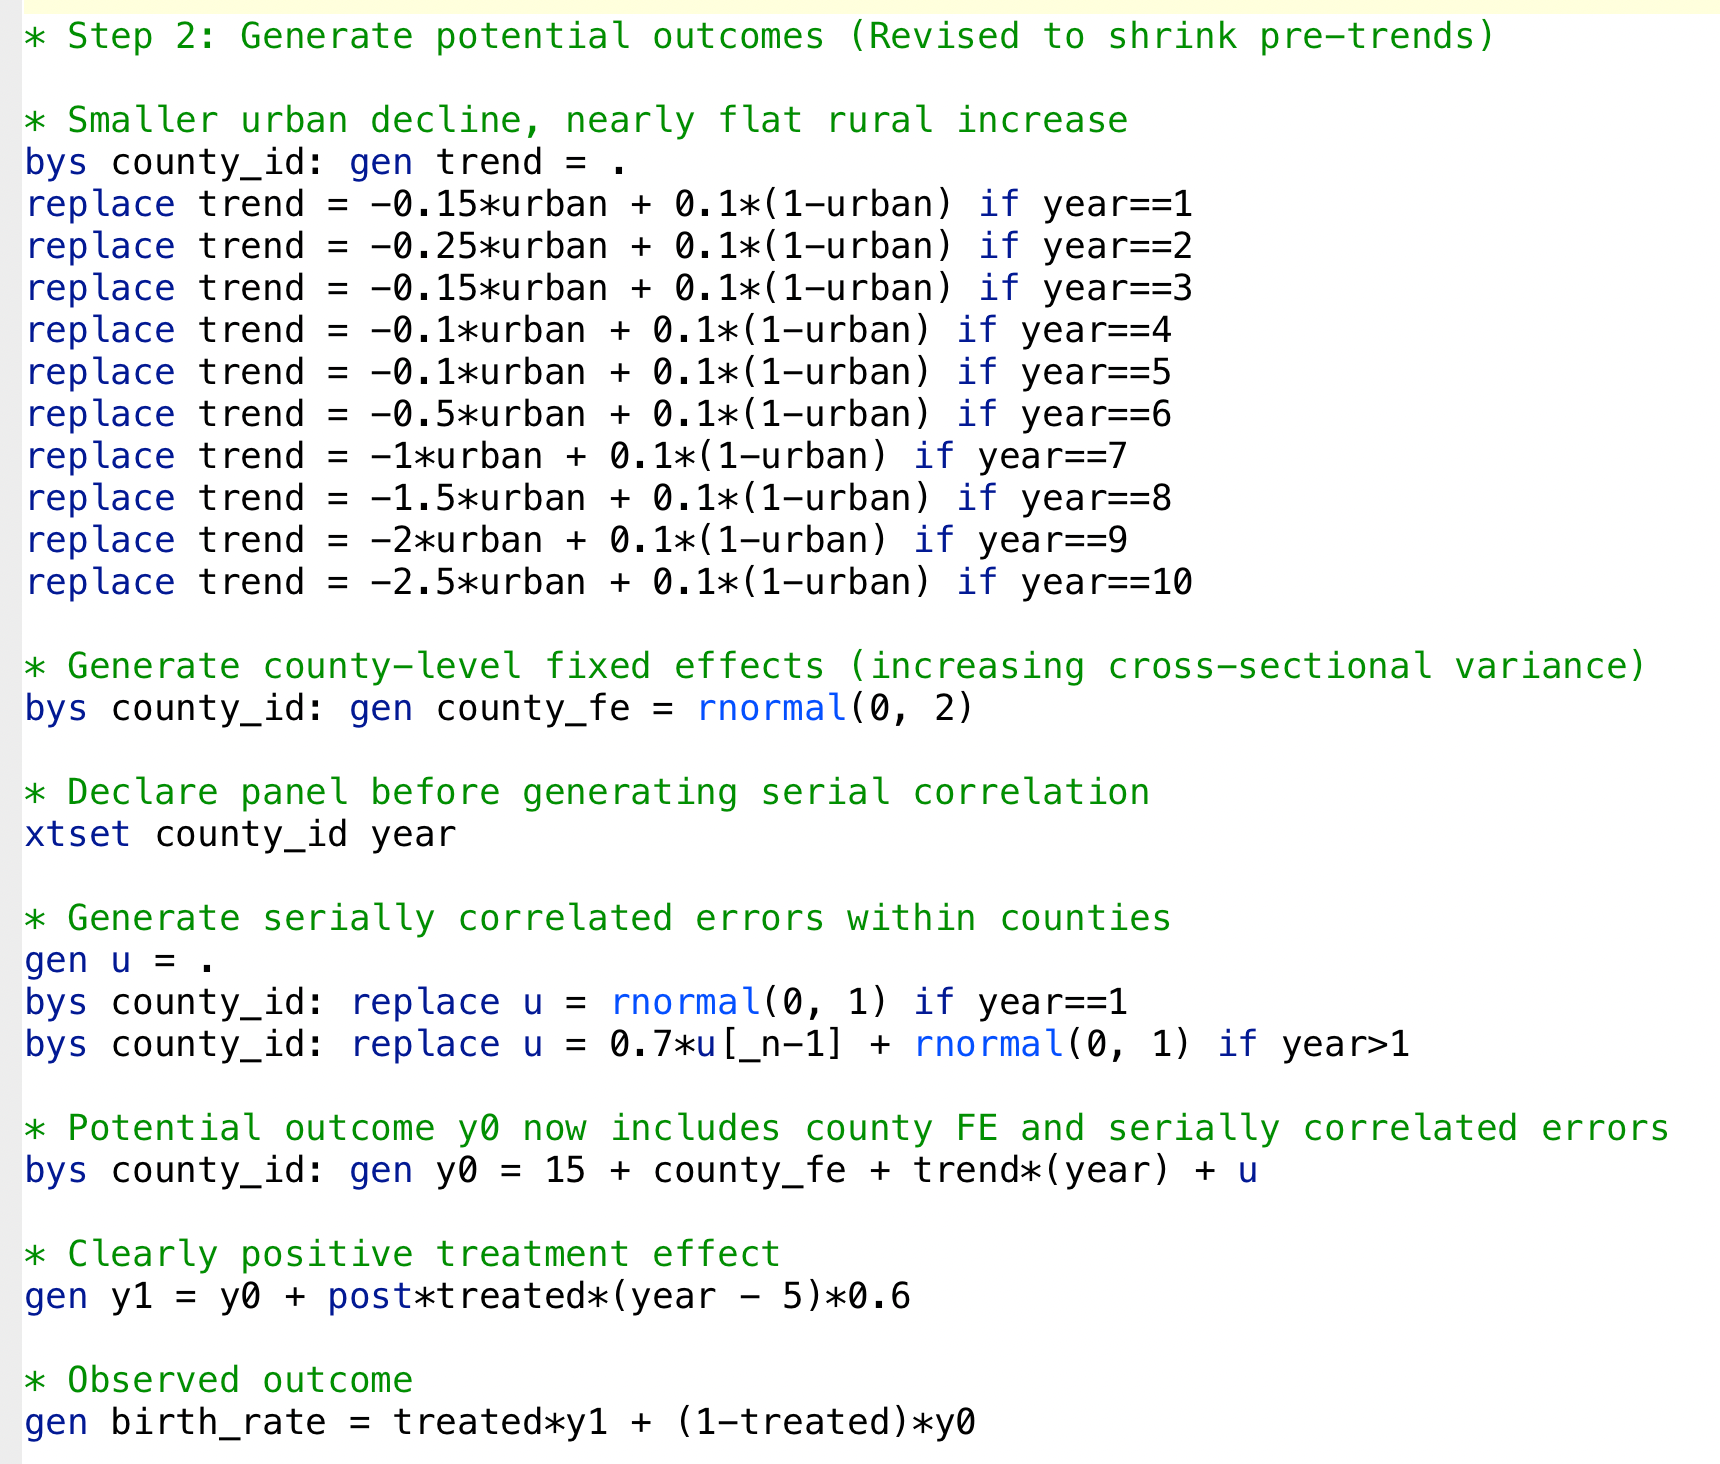
\includegraphics[height=0.75\textheight]{./lecture_includes/misleading_eventstudy_code}
\end{figure}

\end{frame}







\subsection{NSW}

\begin{frame}{Application using real data}

\begin{itemize}
\item Let's now use a real example with real data and see how well this does
\item Famous paper in AER by Lalonde (1986), an Orley and Card student at Princeton
\item Found that most program evaluation did badly, but let's revisit it with diff-in-diff
\end{itemize}

\end{frame}

\begin{frame}{Description of NSW Job Trainings Program}
	
The National Supported Work Demonstration (NSW), operated by Manpower Demonstration Research Corp in the mid-1970s:
	\begin{itemize}
	\item was a temporary employment program designed to help disadvantaged workers lacking basic job skills move into the labor market by giving them work experience and counseling in a sheltered environment
	\item was also unique in that it \textbf{randomly assigned} qualified applicants to training positions:
		\begin{itemize}
		\item \textbf{Treatment group}: received all the benefits of NSW program
		\item \textbf{Control group}: left to fend for themselves
		\end{itemize}
	\item admitted AFDC females, ex-drug addicts, ex-criminal offenders, and high school dropouts of both sexes
	\end{itemize}
\end{frame}

\begin{frame}{NSW Program}
	
	\begin{itemize}
	\item Treatment group members were:
		\begin{itemize}
		\item guaranteed a job for 9-18 months depending on the target group and site
		\item divided into crews of 3-5 participants who worked together and met frequently with an NSW counselor to discuss grievances and performance
		\item paid for their work
		\end{itemize}
	\item Control group members were randomized so the same
	\item Note: the randomization balanced observables and unobservables across the two arms, thus enabling the estimation of an ATE for the people who self-selected into the program
	\end{itemize}
\end{frame}

\begin{frame}{NSW Program}

\begin{itemize}
	\item Other details about the NSW program:
		\begin{itemize}
		\item \underline{Wages}:  NSW offered the trainees lower wage rates than they would've received on a regular job, but allowed their earnings to increase for satisfactory performance and attendance
		\item \underline{Post-treatment}: after their term expired, they were forced to find regular employment
		\item \underline{Job types}:  varied within sites -- gas station attendant, working at a printer shop -- and males and females were frequently performing different kinds of work
		\end{itemize}
\end{itemize}

\end{frame}
	
\begin{frame}{NSW Data}
	
	\begin{itemize}
	\item \underline{NSW data collection}:
		\begin{itemize}
		\item MDRC collected earnings and demographic information from both treatment and control at baseline and every 9 months thereafter
		\item Conducted up to 4 post-baseline interviews
		\item Different sample sizes from study to study can be confusing, but has simple explanations
		\end{itemize}
	\end{itemize}
\end{frame}
	

\begin{frame}{NSW Data}

\begin{itemize}
	\item \underline{Estimation}:
		\begin{itemize}
		\item NSW was a randomized job trainings program; therefore estimating the average treatment effect is straightforward:
			\begin{eqnarray*}
			\frac{1}{N_t}\sum_{D_i=1}Y_i - \frac{1}{N_c}\sum_{D_i=0}Y_i \approx E[Y^1-Y^0] 
			\end{eqnarray*}in large samples assuming treatment selection is independent of potential outcomes (randomization) -- i.e., $(Y^0,Y^1)\independent{D}$. 
		\end{itemize}
	\item \underline{NSW worked}: Treatment group participants' real earnings post-treatment (1978) was positive and economically meaningful -- $\approx$ \$900 (LaLonde 1986) to \$1,800 (Dehejia and Wahba 2002) depending on the sample used
\end{itemize}

\end{frame}
	
\begin{frame}[plain]
	\begin{center}
	LaLonde, Robert J. (1986). \myurlshort{http://business.baylor.edu/scott_cunningham/teaching/lalonde-1986.pdf}{``Evaluating the Econometric Evaluations of Training Programs with Experimental Data''}. \emph{American Economic Review}. 
	\end{center}
	
\underline{LaLonde's study} was \textbf{not} an evaluation of the NSW program, as that had been done, but rather an evaluation of econometric models done by:
		\begin{itemize}
		\item replacing the experimental NSW control group with non-experimental control group drawn from two nationally representative survey datasets: Current Population Survey (CPS) and Panel Study of Income Dynamics (PSID)
		\item estimating the average effect using non-experimental workers as controls for the NSW trainees 
		\item comparing his non-experimental estimates to the experimental estimates of \$900
		\end{itemize}
\end{frame}

\begin{frame}{LaLonde (1986)}

\begin{itemize}

	\item \underline{LaLonde's conclusion}: available econometric approaches were biased and inconsistent
		\begin{itemize}
		\item His estimates were way off and usually the wrong sign
		\item Conclusion was influential in policy circles and led to greater push for more experimental evaluations
		\end{itemize}

\end{itemize}

\end{frame}

\imageframe{./lecture_includes/lalonde_table5a.png}
\imageframe{./lecture_includes/lalonde_table5b.png}

\begin{frame}[plain,shrink=10]{Imbalanced covariates for experimental and non-experimental samples}

    \begin{center}
		\begin{table}
		\begin{tabular}{lcccccc}
		\hline \hline
		\multicolumn{3}{c}{}&
		\multicolumn{1}{c}{CPS}&
		\multicolumn{1}{c}{NSW}\\
		
		\multicolumn{1}{c}{}&
		\multicolumn{2}{c}{All} &
		\multicolumn{1}{c}{Controls} &
		\multicolumn{1}{c}{Trainees} \\

		\multicolumn{3}{c}{}&
		\multicolumn{1}{c}{$N_c=15,992$}&
		\multicolumn{1}{c}{$N_t=297$}&
		\multicolumn{1}{c}{}&
		\multicolumn{1}{c}{}\\

		\multicolumn{1}{l}{covariate}&
		\multicolumn{1}{c}{mean}&
		\multicolumn{1}{c}{(s.d.)}&
		\multicolumn{1}{c}{mean}&
		\multicolumn{1}{c}{mean}&
		\multicolumn{1}{c}{t-stat}&
		\multicolumn{1}{c}{diff}\\
		\hline
Black    & 0.09 & 0.28 & 0.07 & 0.80 & 47.04 & -0.73\\
Hispanic & 0.07 & 0.26 & 0.07 & 0.94 & 1.47 & -0.02\\
Age & 33.07 & 11.04 & 33.2 & 24.63 & 13.37  & 8.6\\
Married & 0.70 & 0.46 & 0.71 & 0.17 & 20.54 & 0.54\\
No degree & 0.30 & 0.46 & 0.30 & 0.73 & 16.27 & -0.43\\
Education & 12.0 & 2.86 & 12.03 & 10.38 & 9.85 & 1.65 \\
1975 Earnings   & 13.51 & 9.31 & 13.65 & 3.1 & 19.63 & 10.6\\
1975 Unemp  & 0.11 & 0.32 & 0.11 & 0.37 & 14.29 & -0.26\\
		\hline 
		\end{tabular}
		\end{table}
    \end{center}

\end{frame}


\begin{frame}{Lab}

\url{https://github.com/Mixtape-Sessions/Causal-Inference-2/tree/main/Lab/Lalonde}

\bigskip

Together let's do questions 1 and 2a-c

\end{frame}




\begin{frame}{Concluding remarks}

\begin{itemize}
\item Including covariates in a DiD design is done for reasons that are different than in regressions more generally -- we are trying to address a parallel trends violation
\item Typical regression modeling can only incorporate covariates, but that places restrictions on the model, whereas other methods will not
\item We use baseline covariates because we cannot include covariates that are outcomes otherwise it introduces its own biases
\item Doubly robust and IPW incorporate covariates through propensity scores and outcome regressions (or both) using baseline covariate means only
\end{itemize}

\end{frame}

\begin{frame}{Suggestions}

\begin{itemize}

\item Remember that the threat to validity comes from comparing aggregate groups of units for whom differences in observables, with different associations with $Y^0$, violate parallel trends
\item Conditional parallel trends simply requires that groups which are comparable on covariates are more likely to have comparable $Y^0$ trends
\item Check for imbalance at baseline using normalized differences
\item Choose covariates that are highly predictive of the missing potential outcome, $Y^0$

\end{itemize}

\end{frame}



\section{Differential timing} 

\begin{frame}{Handling Differential Timing}

\begin{itemize}
\item What if there had not been just one treatment cohort, but several? 
\item Think of there being three options with differential timing 
	\begin{enumerate}
	\item Traditional twoway fixed effects (TWFE)
	\item Aggregating ATT(g,t) using Callaway and Sant'Anna or Sun and Abraham
	\item Imputation using Borusyak, Jaravel and Speiss, Gardner or Wooldridge
	\end{enumerate}
\item  Let's review now the differential timing literature with an aim to making a decision among them
\end{itemize}

\end{frame}

\begin{frame}{Three Estimators}

\begin{enumerate}
\item Twoway fixed effects (Goodman-Bacon 2021)
\item Callaway and Sant'Anna (2021), or CS
\item Sun and Abraham (2021), or SA
\end{enumerate}

There are several others, but for time I'll focus on these. 
\end{frame}


\subsection{Bacon decomposition}

\begin{frame}{Twoway fixed effects}

\begin{itemize}
\item When working with panel data, the so-called TWFE estimator is the workhorse estimator
\item It's easy to implement, handles time-varying treatments, has a relatively straightforward interpretation under constant treatment effects, standard errors are easy to calculate and understand
\item Interpretation is more complicated with heterogenous treatment effects
\end{itemize}

\end{frame}




\begin{frame}{Discussion of estimate}


$$Y_{ist} = \beta_0 + \delta D_{ist} + \tau_t + \sigma_s + \varepsilon_{ist}$$


\begin{itemize}
\item If you estimate with OLS with differential timing, what does $\widehat{\delta}$ correspond to?
\item It is a weighted average of all possible ``four averages and three subtractions'' 
\item So similar to the 2x2 regression, except the coefficient is a weighted average over several -- including one that we should have avoided all along

\end{itemize}

\end{frame}




\begin{frame}{$K^2$ distinct DDs}

Let's look at 3 timing groups (a, b and c) and one untreated group (U).  With 3 timing groups, there are 9 2x2 DDs.  Here they are:


\begin{center}
\begin{tabular}{c|c|c}
\multicolumn{1}{l}{} &
\multicolumn{1}{l}{} &
\multicolumn{1}{l}{} \\
\midrule
a to b & b to a & c to a \\
a to c & b to c & c to b \\
a to U & b to U & c to U \\
\midrule
\end{tabular}
\end{center}

\bigskip

Let's return to a simpler example with only two groups -- a $k$ group treated at $t_k^*$ and an $l$ treated at $t_l^*$ plus an never-treated group called the $U$ untreated group
\end{frame} 


\begin{frame}{Terms and notation}

\begin{itemize}
\item Let there be two treatment groups ($k,l$) and one untreated group ($U$)
\item $k,l$ define the groups based on when they receive treatment (differently in time) with k receiving it earlier than $l$
\item Denote $\overline{D}_k$ as the share of time each group spends in treatment status
\item Denote $\widehat{\delta}_{jb}^{2x2}$ as the canonical $2\times 2$ DD estimator for groups $j$ and b where $j$ is the treatment group and $b$ is the comparison group
\end{itemize}

\end{frame}


\imageframe{./lecture_includes/bacon_goodman_2.png}



\begin{frame}[plain]
$$\widehat{\delta}^{2x2}_{kU} = \bigg ( \overline{y}_k^{post(k)} - \overline{y}_k^{pre(k)} \bigg ) - \bigg ( \overline{y}_U^{post(k)} - \overline{y}_U^{pre(k)} \bigg ) $$
	\begin{figure}
	\includegraphics[scale=0.45]{./lecture_includes/bacon_goodman_3.png}
	\end{figure}

\end{frame}

\begin{frame}[plain]
$$\widehat{\delta}^{2x2}_{lU} = \bigg ( \overline{y}_l^{post(l)} - \overline{y}_l^{pre(l)} \bigg ) - \bigg ( \overline{y}_U^{post(l)} - \overline{y}_U^{pre(l)} \bigg ) $$
	\begin{figure}
	\includegraphics[scale=0.45]{./lecture_includes/bacon_goodman_4.png}
	\end{figure}

\end{frame}


\begin{frame}[plain]

$$\delta_{kl}^{2x2,k} = \bigg ( \overline{y}_k^{MID(k,l)} - \overline{y}_k^{Pre(k,l)} \bigg ) - \bigg ( \overline{y}_l^{MID(k,l)} - \overline{y}_l^{PRE(k,l)} \bigg ) $$

	\begin{figure}
	\includegraphics[scale=0.45]{./lecture_includes/bacon_goodman_6.png}
	\end{figure}

\end{frame}

\begin{frame}[plain]
$$\delta_{lk}^{2x2,l} = \bigg ( \overline{y}_l^{POST(k,l)} - \overline{y}_l^{MID(k,l)} \bigg ) - \bigg ( \overline{y}_k^{POST(k,l)} - \overline{y}_k^{MID(k,l)} \bigg ) $$

	\begin{figure}
	\includegraphics[scale=0.4]{./lecture_includes/bacon_goodman_7.png}
	\end{figure}

\end{frame}


	

\begin{frame}{Bacon decomposition}

$$Y_{ist} = \beta_0 + \delta D_{ist} + \tau_t + \sigma_s + \varepsilon_{ist}$$


TWFE estimate of $\widehat{\delta}$ is equal to a weighted average over all group 2x2 (of which there are 4 in this example)
\begin{eqnarray*}	
\widehat{\delta}^{TWFE} = \sum_{k \neq U} s_{kU}\widehat{\delta}_{kU}^{2x2} + \sum_{k \neq U} \sum_{l>k} s_{kl}  \bigg [ \mu_{kl}\widehat{\delta}_{kl}^{2x2,k} + (1-\mu_{kl}) \widehat{\delta}_{lk}^{2x2,l} \bigg]
\end{eqnarray*}where that first 2x2 combines the k compared to U and the l to U (combined to make the equation shorter)

\end{frame}
	


\begin{frame}{Third, the Weights}

 \begin{eqnarray*} s_{ku} &=& \frac{ n_k n_u \overline{D}_k (1- \overline{D}_k ) }{ \widehat{Var} ( \tilde{D}_{it} )} \\
s_{kl} &=& \frac{ n_k n_l (\overline{D}_k - \overline{D}_{l} ) ( 1- ( \overline{D}_k - \overline{D}_{l} )) }{\widehat{Var}(\tilde{D}_{it})} \\
\mu_{kl} &=& \frac{1 - \overline{D}_k }{1 - ( \overline{D}_k - \overline{D}_{l} )}
\end{eqnarray*}where $n$ refer to the panel group shares, $\overline{D}_k (1- \overline{D}_k )$, as well as $(\overline{D}_k - \overline{D}_{l} ) ( 1- ( \overline{D}_k - \overline{D}_{l} ))$ expressions refer to variance of treatment, and the final equation is the same for two timing groups.

\end{frame}

\begin{frame}{Weights discussion}

\begin{itemize}
\item Two things to note:
	\begin{itemize}
	\item More units in a group, the bigger its 2x2 weight is
	\item Group treatment variance weights up or down a group's 2x2
	\end{itemize}
\item Think about what causes the treatment variance to be as big as possible. Let's think about the $s_{ku}$ weights.
	\begin{itemize}
	\item $\overline{D}=0.1$. Then $0.1 \times 0.9 = 0.09$
	\item $\overline{D}=0.4$. Then $0.4 \times 0.6 =0.24$
	\item $\overline{D}=0.5$. Then $0.5 \times 0.5 = 0.25$
	\item $\overline{D}=0.6$. Then $0.6 \times 0.4 = 0.24$
	\end{itemize}
\item This means the weight on treatment variance is maximized for \emph{groups treated in middle of the panel}
\end{itemize}
\end{frame}

\begin{frame}{More weights discussion}

\begin{itemize}
\item But what about the ``treated on treated'' weights (i.e., $\overline{D}_k - \overline{D}_{l} $)  
\item Same principle as before - when the difference between treatment variance is close to 0.5, those 2x2s are given the greatest weight
\item For instance, say $t^*_k=0.15$ and $t^*_l=0.67$. Then $\overline{D}_k - \overline{D}_{l} = 0.52$.  And thus $0.52 \times 0.48 = 0.2496$.
\end{itemize}

\end{frame}


\begin{frame}{Summarizing TWFE centralities}

\begin{itemize}
\item Groups in the middle of the panel weight up their respective 2x2s via the variance weighting
\item Decomposition highlights the strange role of panel length when using TWFE
\item Different choices about panel length change both the 2x2 and the weights based on variance of treatment
\end{itemize}

\end{frame}




\begin{frame}{Back to TWFE}


$$Y_{ist} = \beta_0 + \delta D_{ist} + \tau_t + \sigma_s + \varepsilon_{ist}$$


\begin{itemize}

\item So we know that the estimate is a weighted average over all ``four averages and three subtractions'' but is that good or bad?
\item It's good if it's unbiased; it's bad if it isn't, and the decomposition doesn't tell us which unless we replace realized outcomes with potential outcomes
\item Bacon shows that TWFE estimate of $\delta$ needs two assumptions for unbiasedness:
	\begin{enumerate}
	\item variance weighted parallel trends are zero and 
	\item no dynamic treatment effects (not the case with 2x2)
	\end{enumerate}
\item Under those assumptions, TWFE estimator estimates the variance weighted ATT as a weighted average of all possible ATTs (not just weighted average of DiDs)

\end{itemize}

\end{frame}


\begin{frame}{Moving from 2x2s to causal effects and bias terms}

Let's start breaking down these estimators into their corresponding estimation objects expressed in causal effects and biases


\begin{eqnarray*}
\widehat{\delta}^{2x2}_{kU} &=& ATT_k{Post} + \Delta Y^0_k(Post(k),Pre(k)) - \Delta Y^0_U(Post(k),Pre) \\
\widehat{\delta}^{2x2}_{kl} &=& ATT_k(MID) + \Delta Y^0_k(MID,Pre) - \Delta Y^0_l(MID, Pre)
\end{eqnarray*}These look the same because you're always comparing the treated unit with an untreated unit (though in the second case it's just that they haven't been treated \emph{yet}). 

\end{frame}

\begin{frame}{The dangerous 2x2}

But what about the 2x2 that compared the late groups to the already-treated earlier groups? With a lot of substitutions we get:

\begin{eqnarray*}
\widehat{\delta}^{2x2}_{lk} &=& ATT_{l,Post(l)} + \underbrace{\Delta Y^0_l(Post(l),MID) - \Delta Y^0_k ( Post(l), MID)}_{\mathclap{\text{Parallel trends bias}}} \\
&& - \underbrace{(ATT_k(Post) - ATT_k(Mid))}_{\mathclap{\text{Heterogeneity bias!}}}
\end{eqnarray*}


\end{frame}

\begin{frame}{Substitute all this stuff into the decomposition formula}

\begin{eqnarray*}	
\widehat{\delta}^{TWFE} = \sum_{k \neq U} s_{kU}\widehat{\delta}_{kU}^{2x2} + \sum_{k \neq U} \sum_{l>k} s_{kl}  \bigg [ \mu_{kl}\widehat{\delta}_{kl}^{2x2,k} + (1-\mu_{kl}) \widehat{\delta}_{kl}^{2x2,l} \bigg]
\end{eqnarray*}where we will make these substitutions\begin{eqnarray*}
\widehat{\delta}_{kU}^{2x2} &=& ATT_k(Post) + \Delta Y_k^0(Post,Pre) - \Delta Y_U^0(Post, Pre) \\
\widehat{\delta}_{kl}^{2x2,k} &=& ATT_k(Mid) + \Delta Y_k^0(Mid,Pre) - \Delta Y_l^0(Mid, Pre) \\
\widehat{\delta}^{2x2,l}_{lk} &=& ATT_{l}Post(l) + \Delta Y^0_l(Post(l),MID) - \Delta Y^0_k ( Post(l), MID) \\
&&- (ATT_k(Post) - ATT_k(Mid))
\end{eqnarray*}Notice all those potential sources of biases! 

\end{frame}


\begin{frame}{Potential Outcome Notation}

\begin{eqnarray*}
p\text{ }lim\text{ } \widehat{\delta}^{TWFE}_{n\to\infty} &=& VWATT + VWPT - \Delta ATT
\end{eqnarray*}

\begin{itemize}
\item Notice the number of assumptions needed \emph{even} to estimate this very strange weighted ATT (which is a function of how you drew the panel in the first place). 
\item With dynamics, it attenuates the estimate (bias) and can even reverse sign depending on the magnitudes of what is otherwise effects in the sign in a reinforcing direction! 
\item Model can flip signs (does not satisfy a ``no sign flip property'')
\end{itemize}

\end{frame}






\begin{frame}{Simulated data}

\begin{itemize}
\item 1000 firms, 40 states, 25 firms per states, 1980 to 2009 or 30 years, 30,000 observations, four groups

\item I'll impose ``unit level parallel trends'', which is much stronger than we need (we only need average parallel trends)

\item Also no anticipation of treatment effects until treatment occurs but does \emph{not} guarantee homogenous treatment effects

\item Two types of situations: constant versus dynamic treatment effects
\end{itemize}
\end{frame}



\begin{frame}{Constant vs Dynamic Treatment Effects}
    \begin{columns}
        \column{0.5\linewidth}
        \centering
        \includegraphics[height=6.5cm, width=5.5cm]{./lecture_includes/constant_te}

        \column{0.5\linewidth}
        \centering
        \includegraphics[height=6.5cm, width=5.5cm]{./lecture_includes/dynamic_te}
    \end{columns} 
\end{frame}



\begin{frame}{Group-time ATT}
       \begin{columns}
          \column{0.38\linewidth}
             \centering
             \includegraphics[height=6.5cm, width=5.5cm]{./lecture_includes/baker_attgt}
           \column{0.48\linewidth}
		\begin{itemize}
\item Heterogenous treatment effects across time and across groups
\item Cells are called ``group-time ATT'' (Callaway and Sant'Anna 2021) or ``cohort ATT'' (Sun and Abraham 2021)
\item ATT is weighted average of all cells and $+82$ with uniform weights $1/60$
		\end{itemize}
         \end{columns} 
    \end{frame}
    
    

\begin{frame}{Estimation}

\bigskip

Estimate the following equation using OLS:

$$Y_{ist} = \alpha_i + \gamma_t +\delta D_{it} + \varepsilon_{ist}$$


\begin{table}[htbp]\centering
\small
\caption{Estimating ATT with different models}
\begin{center}
\begin{tabular}{l*{5}{c}}
\hline
\multicolumn{1}{l}{\textbf{}}&
\multicolumn{1}{c}{\textbf{Truth}}&
\multicolumn{1}{c}{\textbf{(TWFE)}}&
\multicolumn{1}{c}{\textbf{(CS)}}&
\multicolumn{1}{c}{\textbf{(SA)}}&
\multicolumn{1}{c}{\textbf{(BJS)}}\\
\hline
$\widehat{ATT}$  & 82    & -6.69*** &&&\\
\hline
\end{tabular}
\end{center}
\end{table}

The sign flipped.  Why?  Because of \emph{extreme} dynamics (i.e., $- \Delta ATT$)

\end{frame}

\begin{frame}{Bacon decomposition}
\begin{table}[htbp]\centering
\small
\caption{Bacon Decomposition (TWFE $= -6.69$)}
\begin{center}
\begin{tabular}{l*{5}{c}}
\hline
\multicolumn{1}{l}{\textbf{DD Comparison}}&
\multicolumn{1}{l}{\textbf{Weight}}&
\multicolumn{1}{l}{\textbf{Avg DD Est}}\\
\hline
Earlier T vs. Later C  &     0.500   &       51.800 \\
Later T vs. Earlier C   &    0.500    &     -65.180 \\
\midrule
T $=$ Treatment; C$ =$ Comparison \\
$(0.5*51.8) + (0.5*-65.180) = -6.69$ \\
\hline
\end{tabular}
\end{center}
\end{table}

\bigskip

While large weight on the ``late to early 2x2'' is \emph{suggestive} of an issue, these would appear even if we had constant treatment effects

\end{frame}







\subsection{Callaway and Sant'Anna}



\begin{frame}{Callaway and Sant'Anna 2021}

CS is a DiD estimator used with differential timing to estimate "building block" parameters called group-time $ATT(g,t)$ parameters and is used in situations like this:

\begin{enumerate}
\item When treatment effects differ depending on when it was adopted
\item When treatment effects change over time
\item When shortrun treatment effects are different than longrun effects
\end{enumerate}


\end{frame}




\begin{frame}{Group-time ATT}
       \begin{columns}
          \column{0.38\linewidth}
             \centering
             \includegraphics[height=6.5cm, width=5.5cm]{./lecture_includes/baker_attgt}
           \column{0.38\linewidth}
            Each cell contains that group's ATT(g,t)
\begin{eqnarray*}
ATT(g,t) = E[Y_t^1 - Y_t^0 | G_g=1]
\end{eqnarray*}CS identifies all feasible ATT(g,t)
         \end{columns} 
    \end{frame}




\begin{frame}{Group-time ATT}

Group-time ATT is the ATT for a specific group and time
\begin{itemize}
\item Groups are basically cohorts of units treated at the same time
\item Group-time ATT estimates are simple (weighted) differences in means
\item Does not directly restrict heterogeneity with respect to observed covariates, timing or the evolution of treatment effects over time
\item Allows us ways to choose our aggregations
\item Inference is the bootstrap
\end{itemize}

\end{frame}



\begin{frame}{Notation}

\begin{itemize}
\item $T$ periods going from $t=1, \dots, T$
\item Units are either treated ($D_t=1$) or untreated ($D_t=0$) but once treated cannot revert to untreated state
\item $G_g$ signifies a group and is binary.  Equals one if individual units are treated at time period $t$.
\item $C$ is also binary and indicates a control group unit equalling one if ``never treated'' (can be relaxed though to ``not yet treated'')
	\begin{itemize}
	\item Recall the problem with TWFE on using treatment units as controls
	\end{itemize}
\item Generalized propensity score enters into the estimator as a weight: $$\widehat{p(X)} = Pr(G_g=1 | X,G_g+C=1)$$
\end{itemize}

\end{frame}

\begin{frame}{Assumptions}

Assumption 1: Irreversible treatment \\
Assumption 2: Conditional parallel trends (for either never treated or not yet treated) \\
\begin{eqnarray*}
E[Y_t^0 - Y_{t-1}^0 | X,G_g=1] = [Y_t^0 - Y_{t-1}^0 | X,C=1] 
\end{eqnarray*}
\bigskip
Assumption 3: Common support (propensity score) \\
\bigskip
Assumption 4: No Anticipation

\end{frame}

\begin{frame}{CS Estimator (the IPW version)}

\begin{eqnarray*}
ATT(g,t) = E \bigg [ \bigg ( \frac{G_g}{E[G_g]} - \frac{ \frac{\hat{p}(X)C}{1-\hat{p}(X)}}{E \bigg [ \frac{\hat{p}(X)C}{1-\hat{p}(X)} \bigg ]} \bigg ) (Y_t - Y_{g-1} ) \bigg ) \bigg ]
\end{eqnarray*}

This is the inverse probability weighting estimator.  Alternatively, there is an outcome regression approach and a doubly robust. Sant'Anna recommends DR.  CS uses the never-treated or the not-yet-treated as controls but never the already-treated 
\end{frame}




\begin{frame}{Aggregated vs single year/group ATT}

\begin{itemize}
\item The method they propose is really just identifying very narrow ATT per group time.
\item But we are often interested in  more aggregate parameters, like the ATT across all groups and all times
\item They present two alternative methods for building ``interesting parameters'' 
\item Inference from a bootstrap
\end{itemize}


\end{frame}



\begin{frame}{Group-time ATT }
             \includegraphics[scale=0.45]{./lecture_includes/baker_attgt_cs}

Question: Why didn't CS estimate all ATT(g,t)? What is ``feasible ATT''?

\end{frame}

\begin{frame}{Reporting results}
\begin{table}[htbp]\centering
\small
\caption{Estimating ATT using only pre-2004 data}
\begin{center}
\begin{tabular}{l*{5}{c}}
\hline
\multicolumn{1}{l}{\textbf{}}&
\multicolumn{1}{c}{\textbf{(Truth)}}&
\multicolumn{1}{c}{\textbf{(TWFE)}}&
\multicolumn{1}{c}{\textbf{(CS)}}&
\multicolumn{1}{c}{\textbf{(SA)}}&
\multicolumn{1}{c}{\textbf{(BJS)}}\\
\hline
$\widehat{Feasible\ ATT}$  & 68.33    & 26.81 *** & 68.34*** &&\\
\hline
\end{tabular}
\end{center}
\end{table}

TWFE is no longer negative, interestingly, once we eliminate the last group (giving us a never-treated group), but is still suffering from attenuation bias. 

\end{frame}




\begin{frame}{Event study and differential timing}

\begin{itemize}
\item Sometimes we care about a simple summary, and sometimes we care about separating it out in time and sometimes in even more interesting ways
\item Event studies with one treatment group and one untreated group were relatively straightforward
\item Interact treatment group with calendar date to get a series of leads and lags
\item But when there are more than one treatment group, specification challenges emerge
\end{itemize}

\end{frame}





\begin{frame}{Bias of TWFE Event Study Specification}

\begin{itemize}
\item Bacon only focused on the static specification, and that's where the biases due to dynamics revealed itself
\item He was unable to get into the leads and lags using the FWL method he was using (``it's hard!'' - Bacon)
\item Sophie Sun and Sarah Abraham did though -- prompted by a stray comment by their professor
\item But they also unlike Bacon present a solution (which is like CS, but discovered independently)
\end{itemize}

\end{frame}

\begin{frame}{Event study specification with TWFE}


\begin{eqnarray*}
Y_{i,t} = \alpha_i + \delta_t + \sum_{g \in G} \mu_g1\{t-E_i \in g \} + \varepsilon_{i,t}
\end{eqnarray*}

\bigskip

We will focus on the coefficient $\widehat{\mu_g}$ when estimated with TWFE

\end{frame}



\subsection{Sun and Abraham}

\begin{frame}{Sun and Abraham 2021}

	\begin{enumerate}
	\item SA shows a decomposition of the population regression coefficient on event study leads and lags with differential timing estimated with TWFE
	\item They show that the population regression coefficient is ``contaminated'' by information from other leads and lags (which is then later generalized by Goldsmith-Pinkham, Hull and Kolesar 2022)
	\item SA presents an alternative estimator that is a version of CS only using the ``last cohort'' as the comparison group (not the not-yet-treated)
	\item Derives the variance of the estimator instead of bootstrapping, handles covariates differently than CS, but otherwise identical
	\end{enumerate}

\end{frame}

\begin{frame}{Summarizing (cont.)}

\begin{itemize}
\item Under homogenous treatment profiles, weights sum to zero and ``cancel out'' the treatment effects from other periods 
\item Under treatment effect heterogeneity, they do not cancel out and leads and lags are biased
\item They present a 3-step TWFE based alternative estimator which addresses the problems that they find
\end{itemize}

\end{frame}


\begin{frame}{Some notation and terms}

\begin{itemize}
\item As people often \textbf{bin} the data, we allow a lead or lag $l$ to appear in bin $g$ so sometimes they use $g$ instead of $l$ or $l \in g$
\item Building block is the ``cohort-specific ATT'' or $CATT_{e,l}$ -- same as ATT(g,t)
\item Our goal is to estimate $CATT_{l}$ with population regression coefficient $\mu_l$
\item They focus on irreversible treatment where treatment status is non-decreasing sequence of zeroes and ones
\end{itemize}

\end{frame}



\begin{frame}{Difficult notation (cont.)}

\begin{itemize}
\item The $\infty$ symbol is used to either describe the group ($E_i=\infty$) or the potential outcome ($Y^{\infty}$)
\item $Y^{\infty}_{i,t}$ is is the potential outcome for unit $i$ if it had never received treatment (versus received it later), also called the baseline outcome
\item Other counterfactuals are possible -- maybe unit $i$ isn't ``never treated'' but treated later in counterfactual
\end{itemize}
\end{frame}

\begin{frame}{More difficult notation (cont.)}

\begin{itemize}
\item Treatment effects are the difference between the observed outcome relative to the never-treated counterfactual outcome: $Y_{i,t} - Y^{\infty}_{i,t}$
\item We can take the average of treatment effects at a given relative time period across units first treated at time $E_i=e$ (same cohort) which is what we mean by $CATT_{e,l}$
\item Doesn't use $t$ index time (``calendar time''), rather uses $l$ which is time until or time after treatment date $e$ (``relative time'')
\item Think of it as ${l}=$year - treatment date
\end{itemize}

\end{frame}

\begin{frame}{Relative vs calendar event time}


\begin{figure}
\includegraphics[scale=0.2]{./lecture_includes/timetil}
\end{figure}

\end{frame}


\begin{frame}{Definition 1}

\textbf{Definition 1:} The cohort-specific ATT $l$ periods from initial treatment date $e$ is:

\begin{eqnarray*}
CATT_{e,l} = E[Y_{i,e+l} - Y^{\infty}_{i,e+l} | E_i=e]
\end{eqnarray*}

\bigskip

Fill out the second part of the Group-time ATT exercise together.

\end{frame}

\begin{frame}{TWFE assumptions}

\begin{itemize}
\item For consistent estimates of the coefficient leads and lags using TWFE model, we need three assumptions
\item For SA and CS, we only need two
\item Let's look then at the three
\end{itemize}

\end{frame}


\begin{frame}{Assumption 1: Parallel trends}

\textbf{Assumption 1: Parallel trends in baseline outcomes}: $E[Y^{\infty}_{i,t} - Y^{\infty}_{i,s} | E_i = e ]$ is the same for all $e \in supp(E_i)$ and for all $s$, $t$ and is equal to $E[Y^{\infty}_{i,t} - Y^{\infty}_{i,s} ]$

\bigskip

Lead and lag coefficients are DiD equations but once we invoke parallel trends they can become causal parameters.  This reminds us again how crucial it is to have  appropriate controls

\end{frame}


\begin{frame}{Assumption 2: No anticipation}

\textbf{Assumption 2: No anticipator behavior in pre-treatment periods}: There is a set of pre-treatment periods such that $E[Y_{i,e+l}^e - Y_{i,e+l}^{\infty} | E_i = e]=0$ for all possible leads.

\bigskip

Essentially means that pre-treatment, the causal effect is zero.  Most plausible if no one sees the treatment coming, but even if they see it coming, they may not be able to make adjustments that affect outcomes

\end{frame}


\begin{frame}{Assumption 3: Homogeneity}

\textbf{Assumption 3: Treatment effect profile homogeneity}: For each relative time period $l$, the $CATT_{e,l}$ doesn't depend on the cohort and is equal to $CATT_l$. 


\end{frame}

\begin{frame}{Treatment effect heterogeneity}

\begin{itemize}
\item Assumption 3 is violated when different cohorts experience different paths of treatment effects
\item Cohorts may differ in their covariates which affect how they respond to treatment (e.g., if treatment effects vary with age, and there is variation in age across units first treated at different times, then there will be heterogeneous treatment effects)
\item Doesn't rule out parallel trends
\end{itemize}

\end{frame}

\begin{frame}{Event study model}

Dynamic TWFE model

\begin{eqnarray*}
Y_{i,t} = \alpha_i + \delta_t + \sum_{g \in G} \mu_g1\{t-E_i \in g \} + \varepsilon_{i,t}
\end{eqnarray*}

\bigskip

We are interested in the properties of $\mu_g$ under differential timing as well as whether there are any never-treated units

\end{frame}



\begin{frame}[plain, shrink=20]
\begin{center}
\textbf{Interpreting $\widehat{\mu_g}$ under no to all assumptions}
\end{center}

\textbf{Proposition 1 (no assumptions):} The population regression coefficient on relative period bin $g$ is a linear combination of differences in trends from its own relative period $l \in g$, from relative periods $l \in g'$ of other bins $g' \neq g$, and from relative periods excluded from the specification (e.g., trimming). 

\begin{eqnarray*}
\mu_g &=& \underbrace{\sum_{l \in g} \sum_{e} w^g_{e,l} \big ( E[Y_{i,e+l} - Y^{\infty}_{i,0} | E_i = e] - E[Y^{\infty}_{i,e+l} - Y^{\infty}_{i,0}] \big )}_{\mathclap{\text{Targets}}} \\
&+& \underbrace{\sum_{g' \neq g} \sum_{l \in g'} \sum_e w^g_{e,l} \big ( E[Y_{i,e+l} - Y^{\infty}_{i,0} | E_i=e] - E[Y^{\infty}_{i,e+l} - Y^{\infty}_{i,0}] \big )}_{\mathclap{\text{Contamination from other leads and lags}}} \\
&+&  \underbrace{\sum_{l \in g^{excl}} \sum_{e} w^g_{e,l} \big ( E[Y_{i,e+l} - Y^{\infty}_{i,0} | E_i=e] - E[Y^{\infty}_{i,e+l} - Y^{\infty}_{i,0}] \big )}_{\mathclap{\text{Contamination from dropped periods}}} 
\end{eqnarray*}

\bigskip


\end{frame}

\begin{frame}{Weight ($w^g_{e,l}$) summation cheat sheet}

\begin{enumerate}
\item For relative periods of $\mu_g$ own $l \in g$, $\sum_{l \in g}\sum_ew^g_{e,l}=1$
\item For relative periods belonging to some other bin $l\in g'$ and $g' \neq g$, t $\sum_{l \in g'}\sum_ew^g_{e,l} = 0$
\item For relative periods not included in $G$, $\sum_{l \in g^{excl}} \sum_e w^g_{e,l} = -1$
\end{enumerate}

\end{frame}




\begin{frame}{Estimating the weights}

Regress $D^l_{i,t} \times 1\{E_i=e \}$ on:

\begin{enumerate}
\item all bin indicators included in the main TWFE regression, 
\item $\{ 1\{ t-E_i \in g \} \}_{g \in G}$(i.e., leads and lags) and 
\item the unit and time fixed effects
\end{enumerate}

\end{frame}


\begin{frame}{Still biased under parallel trends}

\textbf{Proposition 2}: Under the parallel trends only, the population regression coefficient on the indicator for relative period bing $g$ is a linear combination of $CATT_{e,l \in g}$ as well as $CATT_{d,l'}$ from other relative periods $l' \notin g$ with the same weights stated in Proposition 1:

\begin{eqnarray*}
\mu_g &=& \underbrace{\sum_{l \in g} \sum_e w^g_{e,l} CATT_{e,l}}_{\mathclap{\text{Desirable}}} \\
&& + \underbrace{\sum_{g' \neq g, g' \in G} \sum_{l' \in g'} \sum_e w^g_{e,l'}  CATT_{e,l'}}_{\mathclap{\text{Bias from other specified bins}}} \\
&&+ \underbrace{\sum_{l' \in g^{excl}} \sum_e w^g_{e,l'} CATT_{e,l'}}_{\mathclap{\text{Bias from dropped relative time indicators}}}
\end{eqnarray*}



\end{frame}


\begin{frame}{Still biased under parallel trends and no anticipation}

\textbf{Proposition 3}: If parallel trends holds and no anticipation holds for all $l<0$ (i.e., no anticipatory behavior pre-treatment), then the population regression coefficient $\mu_g$ for $g$ is a linear combination of post-treatment $CATT_{e,l'}$ for all $l' \geq 0$.

\begin{eqnarray*}
\mu_g &=& \sum_{l' \in g, l' \geq 0} \sum_e w^g_{e,l'} CATT_{e,l'} \\
&&+ \sum_{g' \neq g,g' \in G} \sum_{l' \in g', l' \geq 0} \sum_e w^g_{e,l'} CATT_{e,l'} \\
&&+ \sum_{l' \in g^{excl},l' \geq 0} \sum_e w^g_{w,l'} CATT_{e,l'}
\end{eqnarray*}

\end{frame}

\begin{frame}{Proposition 3 comment}

Notice how once we impose zero pre-treatment treatment effects, those terms are gone (i.e., no $l \in g, l<0$).  But the second term remains unless we impose treatment effect homogeneity (homogeneity causes terms due to weights summing to zero to cancel out). Thus $\mu_g$ may be non-zero for pre-treatment periods \emph{even though parallel trends hold in the pre period.}

\end{frame}

\begin{frame}{Proposition 4}

\textbf{Proposition 4}: If parallel trends and treatment effect homogeneity, then $CATT_{e,l}=ATT_l$ is constant across $e$ for a given $l$, and the population regression coefficient $\mu_g$ is equal to a linear combination of $ATT_{l \in g}$, as well as $ATT_{l' \notin g}$ from other relative periods

\begin{eqnarray*}
\mu_g &=& \sum_{l \in g} w^g_l ATT_l \\
&&+ \sum_{g' \neq g} \sum_{l' \in g'} w^g_{l'} ATT_{l'} \\
&&+ \sum_{l' \in g^{excl}} w^g_{l'}ATT_{l'}
\end{eqnarray*}


\end{frame}

\begin{frame}{Simple example}


Balanced panel $T=2$ with cohorts $E_i \in \{1,2 \}$. For illustrative purposes, we will include bins $\{-2,0\}$ in our calculations but drop $\{-1,1\}$. 


\end{frame}

\begin{frame}{Simple example}

\begin{eqnarray*}
\mu_{-2} &=& \underbrace{CATT_{2,-2}}_{\mathclap{\text{own period}}} + \underbrace{\frac{1}{2}CATT_{1,0} - \frac{1}{2} CATT_{2,0}}_{\mathclap{\text{other included bins}}} \\
&&+ \underbrace{ \frac{1}{2} CATT_{1,1} - CATT_{1,-1} - \frac{1}{2} CATT_{2,-1} }_{\mathclap{\text{Excluded bins}}}
\end{eqnarray*}

\begin{itemize}
\item Parallel trends gets us to all of the $CATT$
\item No anticipation makes $CATT=0$ for all $l<0$ (all $l<0$ cancel out)
\item Homogeneity cancels second and third terms
\item Still leaves $\frac{1}{2} CATT_{1,1}$ -- you chose  to exclude a group with a treatment effect
\end{itemize}Lesson: drop the relative time indicators on the left, not things on the right, bc lagged effects will contaminate through the excluded bins


\end{frame}


\begin{frame}{Robust event study estimation}


\begin{itemize}
\item All the robust estimators under differential timing have solutions and they all skip over forbidden contrasts. 
\item Sun and Abraham (2021) propose a 3-step interacted weighted estimator (IW) using last treated group as control group
\item Callaway and Sant'anna (2021) estimate group-time ATT which can be a weighted average over relative time periods too but uses ``not-yet-treated'' as control
\end{itemize}

\end{frame}




\begin{frame}{Interaction-weighted estimator}

\begin{itemize}
\item \textbf{Step one}: Do this DD regression and hold on to $\widehat{\delta}_{e,l}$
\end{itemize}

\begin{eqnarray*}
Y_{i,t} = \alpha_i + \lambda_t + \sum_{e \notin C} \sum_{l \neq -1} \delta_{e,l} \big (1 \{ E_i = e \} \cdot D_{i,t}^l \big ) + \varepsilon_{i,t}
\end{eqnarray*}


\bigskip

Can use never-treated or last-treated cohort. Drop always treated. The $\delta_{e,l}$ is a DD estimator for $CATT_{e,l}$ with particular choices for pre-period and cohort controls

\end{frame}


\begin{frame}{Interaction-weighted estimator}

\begin{itemize}
\item \textbf{Step two}: Estimate weights using sample shares of each cohort in the relevant periods:
\end{itemize}

\begin{eqnarray*}
Pr(E_i=e|E_i \in [-l,T-l])
\end{eqnarray*}

\end{frame}

\begin{frame}{Interaction-weighted estimator}

\begin{itemize}
\item \textbf{Step three}: Take a weighted average of estimates for $CATT_{e,l}$ from Step 1 with weight estimates from step 2
\end{itemize}


\begin{eqnarray*}
\widehat{v}_g = \frac{1}{|g|} \sum_{l \in g} \sum_e \widehat{\delta}_{e,l} \widehat{Pr} \{ E_i=e | E_i \in [-l,T-l]\}
\end{eqnarray*}


\end{frame}

\begin{frame}{Consistency and Inference}


\begin{itemize}
\item Under parallel trends and no anticipation, $\widehat{\delta}_{e,l}$ is consistent, and sample shares are also consistent estimators for population shares. 
\item Thus IW estimator is consistent for a weighted average of $CATT_{e,l}$ with weights equal to the share of each cohort in the relevant period(s).
\item They show that each IW estimator is asymptotically normal and derive its asymptotic variance. Doesn't rely on bootstrap like CS.
\end{itemize}

\end{frame}

\begin{frame}{DD Estimator of CATT}

\textbf{Definition 2}: DD estimator with pre-period $s$ and control cohorts $C$ estimates $CATT_{e,l}$ as:

\begin{eqnarray*}
\widehat{\delta_{e,l}} = \frac{ E_N \big [ \big ( Y_{i, e+l} - Y_{i,s} \big ) \times 1\{E_i=e\} \big ]}{E_N[1 \{E_i=e\} ]} - \frac{E_N \big [ \big ( Y_{i,e+l} \times 1 \{E_i \in C \} ]}{E_N [1 \{ E_i \in C \}]}
\end{eqnarray*}


\textbf{Proposition 5}: If parallel trends and no anticipation both hold for all pre-periods, then the DD estimator using any pre-period and non-empty control cohorts (never-treated or not-yet-treated) is an unbiased estimate for $CATT_{e,l}$

\end{frame}

\begin{frame}{Software}

\begin{itemize}
\item \textbf{Stata}: eventstudyinteract (can be installed from ssc)
\item \textbf{R}: fixest with subab() option (see \url{https://lrberge.github.io/fixest/reference/sunab.html/})
\end{itemize}


\end{frame}


\begin{frame}{Reporting results}
\begin{table}[htbp]\centering
\small
\caption{Estimating ATT}
\begin{center}
\begin{tabular}{l*{4}{c}}
\hline
\multicolumn{1}{l}{\textbf{}}&
\multicolumn{1}{c}{\textbf{(Truth)}}&
\multicolumn{1}{c}{\textbf{(TWFE)}}&
\multicolumn{1}{c}{\textbf{(CS)}}&
\multicolumn{1}{c}{\textbf{(SA)}}\\
\hline
$\widehat{Feasible\ ATT}$  & 68.33    & 26.81*** & 68.34*** & 68.33***\\
\hline
\end{tabular}
\end{center}
\end{table}

\end{frame}

\begin{frame}{Computing relative event time leads and lags }
             \includegraphics[scale=0.45]{./lecture_includes/sa_leads}

Two things to notice: (1) there only 17 lags with robust models but will be 24 with TWFE; (2) changing colors mean what?

\end{frame}

\begin{frame}{Comparing TWFE and SA }

\begin{figure}
\begin{center}
             \includegraphics[scale=0.4]{./lecture_includes/twfe_sa_event}
\end{center}
\end{figure}

Question: why is TWFE \emph{falling} pre-treatment?  Why is SA rising, but jagged, post-treatment?

\end{frame}



\subsection{Facebook and Mental Health Example}

\begin{frame}
\begin{center}
\includegraphics[scale=0.35]{./lecture_includes/facebook_quote}
\end{center}
\end{frame}



\begin{frame}{Mental health and Social Media}

\begin{itemize}
\item Unclear what he means; he may mean there is no experimental evidence
\item Very difficult to imagine a randomized experiment -- especially once the claim out there is that it is harmful, Institutional Review Boards likely wouldn't approve it
\item Quasi-experimental evidence can step in to answer important questions like this
\item Braghieri, Levy and Makarin (2022), ``Social Media and Mental Health'', \emph{American Economic Review}, 112(11): 3660-3693


\end{itemize}

\end{frame}

\begin{frame}{Overview of design and data}

\begin{itemize}
\item Authors take advantage of a clever quirk in Facebook (then ``theFacebook'') targeted different universities from 2004 to 2006
\item They found an online data source that allowed them to pin point precisely when a university was ``treated'' with theFacebook
\item They then linked that data with a longrunning health survey of college students (both before and after) in a very clever way
\item Estimated the effect of a new social media platform's presence at a university on student revealed mental health problems

\end{itemize}

\end{frame}


\begin{frame}{DID in Court}

Five elements of a strong DiD
\begin{enumerate}

\item \textbf{Bite}: \textcolor{red}{Nothing}. They cannot really show much here.  No data on Facebook usage.  They had to rely on anecdote and Facebook as a ``first mover'', but there had been Friendster and MySpace so this does weaken the paper maybe
\item \textbf{Main Results}: Very strong evidence, mostly expressed using rich survey data and questions transformed into z-scores (standard deviations)
\item \textbf{Falsifications}: \textcolor{red}{None}. Authors do not perform falsifications. Remember Miller, Johnson and Wherry looking at Medicaid's effect on Medicare eligible population?  There isn't anything like that here.
\item \textbf{Event studies}: Extremely compelling evidence and robustness across a half dozen different models
\item \textbf{Mechanism}: \textcolor{red}{Very weak in my opinion}

\end{enumerate}

\end{frame}

\begin{frame}{DiD in Court}

\begin{itemize}

\item So in many ways the strength of the project lies in a few areas:
	\begin{enumerate}
	\item Important question -- social media and youth mental health problems is a major policy question (see Zuckerberg testifying before Congress about it)
	\item Excellent research design -- difference-in-differences
	\item Meticulous data collection
	\item Data visualization is compelling
	\end{enumerate}
\item And it publishes in the premiere journal in economics, which I think shows that the research question and high quality data combined with research design can lift a paper

\end{itemize}

\end{frame}







\begin{frame}{TWFE}

\begin{equation}
Y_{icgt} = \alpha_g + \delta_t + \beta \times Facebook_{gt} + X_i \times \gamma + X_c \times \psi + \varepsilon_{icgt}
\end{equation}

\bigskip

This is a version of the regression model we looked at called "twoway fixed effects".  Somewhat complicated to dig into, so I will just say that they use it plus some other methods that are appropriate when you have several difference-in-differences events.  But the focus is on $\beta$

\end{frame}


\begin{frame}{Data on Facebook}

\begin{itemize}

\item When does Facebook appear at a school?  
	\begin{itemize}
	\item Facebook only publishes a fraction of that information
	\item They came up with a workaround
	\end{itemize}
\item The Wayback Machine has been taking almost daily photographs of every website since the Internet's beginning -- including the frontpage of ``TheFacebook''
\item Guess what was on the front page of TheFacebook \dots

\end{itemize}

\end{frame}

\begin{frame}
\begin{center}
\includegraphics[scale=0.25]{./lecture_includes/wayback1}
\end{center}
\end{frame}

\begin{frame}
\begin{center}
\includegraphics[scale=0.35]{./lecture_includes/wayback2}
\end{center}
\end{frame}

\begin{frame}
\begin{center}
\includegraphics[scale=0.25]{./lecture_includes/wayback3}
\end{center}
\end{frame}

\begin{frame}
\begin{center}
\includegraphics[scale=0.25]{./lecture_includes/wayback4}
\end{center}
\end{frame}

\begin{frame}{Timing Dates}

\begin{itemize}
\item They went through three years of daily screenshots on Wayback machine to find when a school appeared on the front page
\item The first time Agnes Scott, or Covenant, appears on the front page, the authors mark that as the date when the school got Facebook
\item But now they need information on mental health outcomes
\item They find it with an old long running repeated cross section survey of college students
\end{itemize}

\end{frame}

\begin{frame}{NCHA survey by ACHA}

\begin{quote}
Our second main data source consists of more than 430,000 responses to the NCHA survey, a survey administered to college students on a semi-annual basis by the American College Health Association (ACHA). The NCHA survey was developed in 1998 by a team of college health professionals with the purpose of obtaining information from college students about their mental and physical health. Specifically, the NCHA survey inquires about demographics, physical health, \textbf{mental health}, alcohol and drug use, sexual behaviors, and perceptions of these behaviors among one’s peers.
\end{quote}

\end{frame}

\begin{frame}{No evidence of bite}

\begin{quote}
The NCHA survey does not include any questions on social media use; therefore, it is not possible for us to determine whether a particular survey respondent had a Facebook account.
\end{quote}

\bigskip

This is probably the problem in any study in which your treatment is more or less the first of its kind -- most likely the standard surveys have not yet incorporated the questions into their surveys

\end{frame}

\begin{frame}{Linking Facebook data with NCHA data}

\begin{quote}
In order to protect the privacy of the institutions that participate in the NCHA survey while still allowing us to carry out the analysis, the ACHA kindly agreed to provide us with a customized dataset that includes a variable indicating the semester in which Facebook was rolled out at each college. Specifically, the ACHA adopted the following procedure: (i) merge our dataset containing the Facebook introduction dates to the NCHA dataset; (ii) add a variable listing the semester in which Facebook was rolled out at each college;15 (iii) strip away any information that could allow us to identify colleges (including the specific date in which Facebook was introduced at each college).
\end{quote}

\end{frame}

\begin{frame}{Basic facts about early and late adopters}

\begin{itemize}
\item Colleges in earlier Facebook expansion groups are more selective in terms of test scores, larger, more likely to be on the East Coast, and have more residential undergraduate programs than colleges in later Facebook expansion groups. 

\item Colleges in earlier Facebook expansion groups enroll students from relatively more advantaged economic backgrounds. 

\item Students in colleges that received Facebook relatively earlier have worse baseline mental health outcomes than students attending colleges in later Facebook expansion groups. 

%The baseline differences across Facebook expansion groups may lead one to wonder about the plausibility of the parallel trends assumption in this setting; we address concerns related to parallel trends in Section III.

\end{itemize}

\end{frame}

\begin{frame}{Measurement}

\begin{itemize}
\item The survey data is very rich with a lot of questions about mental health with different scales
\item They create their own combinations of these questions into aggregate indices -- ``index of poor mental health'' where higher numbers mean worse mental health
\item Each outcome survey question is normalized into what is called a ``z-score'' which is interpreted as a fraction of a standard deviation
\item Estimates are ATT parameters -- average effect of Facebook on students at schools that got Facebook
\end{itemize}

\end{frame}


\begin{frame}
\begin{center}
\includegraphics[scale=0.35]{./lecture_includes/facebook_1}
\end{center}
\end{frame}

\begin{frame}
\begin{center}
\includegraphics[scale=0.35]{./lecture_includes/facebook_2}
\end{center}
\end{frame}

\begin{frame}
\begin{center}
\includegraphics[scale=0.35]{./lecture_includes/facebook_3}
\end{center}
\end{frame}

\begin{frame}
\begin{center}
\includegraphics[scale=0.35]{./lecture_includes/facebook_4}
\end{center}
\end{frame}

\begin{frame}
\begin{center}
\includegraphics[scale=0.35]{./lecture_includes/facebook_5}
\end{center}
\end{frame}

\begin{frame}
\begin{center}
\includegraphics[scale=0.35]{./lecture_includes/facebook_6}
\end{center}
\end{frame}

\begin{frame}
\begin{center}
\includegraphics[scale=0.35]{./lecture_includes/facebook_7}
\end{center}
\end{frame}





\section{Don't Do Diff-in-Diff, or DDDiD}



\begin{frame}{Step 10: "Don't Do Diff-in-Diff}

\begin{itemize}
\item If you simply cannot satisfy yourself that the parallel trends assumption holds because there is no adequate comparison group, or whatever, you have to punt on diff-in-diff
\item But that's okay because the goal was never to use diff-in-diff -- the goal was to get an estimated effect of a parameter you wanted to know that was credible
\item You'll probably end up at step 10 more if you introduce a design stage, but that's not the end of the world, because there's still other panel methods (e.g., synthetic control)


\end{itemize}

\end{frame}

\begin{frame}{Replacing Control With Design Time}

\begin{itemize}
\item We often get distracted by shiny objects:
	\begin{itemize}
	\item If only I was better at programming in advanced languages
	\item If only I knew all of the latest methods in causal inference and econometrics
	\end{itemize}
\item Programming and econometrics without a design stage does not create those warranted beliefs
\end{itemize}

\end{frame}




\begin{frame}{Design Trumps Analysis}

	\begin{figure}
	\includegraphics[scale=0.3]{./lecture_includes/rubin_design_trump}
	\end{figure}

\end{frame}


\begin{frame}{Design Trumps Analysis}

\begin{itemize}

\item Your goal is \emph{credible answers} and it's helpful to have the RCT in your mind for many reasons
\item One reason is that RCT teaches us what works -- randomization
\item But another reason is that \emph{designing} RCTs is independently a gold standard -- those researchers are meticulous, even going so far as to submit their \emph{designs} to a journal before doing the analysis
\item No reason we can't do that -- I did that in Ozler, et al (2021) in \emph{Journal of Development Economics}
\item Key for me has been to love all parts of research, including design, love the scientific methods we have been given, love growing and learning, enjoy the process -- that's really the only part we can control
\end{itemize}

\end{frame}


\begin{frame}{Current Practices}
 
\begin{figure}
    \centering
    \includegraphics[width=\textwidth]{./lecture_includes/design_stage}
\end{figure}

\end{frame}



\end{document}


